% Preamble
\documentclass[openany]{book}
\usepackage[a4paper, portrait, margin=2cm]{geometry} % Page size
\usepackage[Lenny]{fncychap}
\usepackage[table]{xcolor} % Colour settings
\usepackage[australian]{babel} % Language settings
% \usepackage{diagrams}
% \usepackage{changes}
\usepackage{essentials}
% \usepackage{extras}
\usepackage{tables}
% \usepackage{preamble/bibliography} % BibLaTeX
% \usepackage{mathptmx}
\usepackage{libertine}
\usepackage[libertine]{newtxmath}
\usepackage{inconsolata}
% \usepackage{libertinus}
% \usepackage{newtx}
\usepackage[noend]{algpseudocode}
\usepackage{listings}
\usepackage{tkz-graph}
\usepackage{tikz-cd}
\usepackage[nottoc,notlot,notlof]{tocbibind}
% \usetikzlibrary{bbox}
% \renewcommand{\VertexSmallMinSize}{8pt}
\usepackage{scalerel}
\usepackage{doi}
% \usepackage{svg}
% \RequirePackage{fix-cm} % arbitrary font scaling
\usepackage{accsupp}
\newcommand{\emptyaccsupp}[1]{\BeginAccSupp{ActualText={}}#1\EndAccSupp{}}
% \DeclareMathSizes{10}{10}{7}{4}

\def\TITLE{Minimum bases for permutation groups}
\def\AUTHOR{Lawrence Chen}
\def\DATE{\today}
% \def\VERSION{Version}

% Settings and commands
\input{commands.tex}
% \input{commands_extras.tex}
\input{commands_tables.tex}
% \input{commands_diagrams.tex}
% Default settings
\allowdisplaybreaks
\frenchspacing
% \renewcommand{\familydefault}{\sfdefault} % Sans Serif
\renewcommand{\arraystretch}{0.8}

% Settings to run at start of document 
\AtBeginDocument{
  \setlength{\doublerulesep}{0.5pt}
  \setlength{\textfloatsep}{-1cm}
  \setlength{\abovedisplayskip}{5pt}
  \setlength{\belowdisplayskip}{5pt}}

% Paragraph spacing settings
\linespread{1.2}
\setlength{\parskip}{0.5em}
% \setlength{\parindent}{0pt} % No paragraph indent

\renewenvironment{quote}{%
  \list{}{%
    \leftmargin3cm   % this is the adjusting screw
    \rightmargin\leftmargin
  }
  \item\relax
}
{\endlist}

% Header and footer
\pagestyle{fancy}
\lhead{}
\rhead{}
\fancyhead[LE]{\itshape\nouppercase\leftmark}
\fancyhead[LO,RE]{}
\fancyhead[RO]{\itshape\nouppercase\rightmark}
% \lhead{\TITLE}
% \rhead{\DATE}
% \lfoot{\VERSION}
% \rfoot{\AUTHOR}
% \patchcmd{\chapter}{\thispagestyle{plain}}{\thispagestyle{fancy}}{}{}

% Theorems
% \theoremstyle{definition}
% \theoremsymbol{\ensuremath\square}
\theorempostskip{\topskip}
% \theorempostskip{0pt}
\declaretheorem[name=Definition, refname=Definition, numberwithin=chapter, style=definition]{definition}
\declaretheorem[name=Axiom, refname=Axiom, numberwithin=section]{axiom}
\renewcommand{\theaxiom}{\arabic{axiom}}
\declaretheorem[name=Proposition, refname=Proposition, sibling=definition]{proposition}
\declaretheorem[name=Theorem, refname=Theorem, sibling=definition]{theorem}
\declaretheorem[name=Corollary, refname=Corollary, sibling=definition]{corollary}
\declaretheorem[name=Lemma, refname=Lemma, sibling=definition]{lemma}
\declaretheorem[name=Remark, refname=Remark, sibling=definition, style=remark]{remark}
\declaretheorem[name=Algorithm, refname=Algorithm, sibling=definition]{algorithm}
\declaretheorem[name=Conjecture, refname=Conjecture, sibling=definition]{conjecture}
\declaretheorem[name=Example, refname=Example, sibling=definition, style=definition]{example}
\declaretheorem[name=Question, refname=Question, sibling=definition]{question}


% Package settings

%% enumerate
% \setlist[itemize]{topsep=0pt}
% \setlist[enumerate]{topsep=0pt}
\setlist[itemize]{topsep=0pt, itemsep=0pt}
\setlist[enumerate]{topsep=0pt, itemsep=0pt}

%% hyperref
\hypersetup{colorlinks=true, linkcolor=blue}

%% tcolorbox
\tcbuselibrary{breakable}
\newtcolorbox{framedbox}{standard jigsaw, opacityback=0, boxrule=1pt, breakable, before skip=8pt, after skip=8pt}

%% tkz-graph
% \GraphInit[vstyle=Hasse]
\GraphInit[vstyle=Welsh]
\SetGraphUnit{1}
\SetVertexMath
\tikzset{VertexStyle/.append style={minimum size=8pt}}

%% listings
% Code block styles (listings)
\definecolor{codegreen}{rgb}{0,0.6,0}
\definecolor{codegray}{rgb}{0.5,0.5,0.5}
\definecolor{codepurple}{rgb}{0.58,0,0.82}
\definecolor{backcolour}{rgb}{0.95,0.95,0.92}
\lstdefinestyle{default}{
  basewidth={.5em,0.5em},
  basicstyle=\ttfamily,
  breakatwhitespace=false,
  breaklines=true,
  captionpos=b,
  xleftmargin=15pt,
  framexleftmargin=2pt,
  framexrightmargin=2pt,
  keepspaces=true,
  numbers=left,
  numbersep=5pt,
  tabsize=4,
  columns=fullflexible,
  backgroundcolor=\color{backcolour},
  commentstyle=\itshape\color{codegreen},
  keywordstyle=\color{magenta},
  numberstyle=\footnotesize\itshape\color{black}\emptyaccsupp,
  stringstyle=\color{codepurple}
}
\lstset{style=default}
% % Package settings

%% tasks
% \settasks{label-offset=0.8em, label-align=right}

%% tocloft
% \renewcommand{\cftsecleader}{\cftdotfill{\cftdotsep}}

%% pgfplots
% \pgfplotsset{compat=newest}
% \usetikzlibrary{calc, patterns, angles, rightangles, quotes, shapes.geometric, arrows.meta, decorations.markings}
% \usepgfplotslibrary{polar}

%% tkz-euclide
% \tkzSetUpLine[line width=0.4pt]

%% tkz-graph
% \GraphInit[vstyle=Hasse]
% \GraphInit[vstyle=Welsh]
% \SetGraphUnit{1}
% \SetVertexMath
% \tikzset{VertexStyle/.append style={minimum size=8pt}}

%% tocloft
% \renewcommand{\cftsecleader}{\cftdotfill{\cftdotsep}}

%% mdframed
% \mdfsetup{skipabove=\topskip, skipbelow=\topskip, innertopmargin=10pt, innerbottommargin=10pt}

%% colortbl
% \arrayrulecolor{gray}

%% cancel
% \renewcommand{\CancelColor}{\color{black}}

%% multiaudience
% \SetNewAudience{default}
% \SetNewAudience{solutions}
% \DefCurrentAudience{solutions}

%% hyperref
% \hypersetup{colorlinks=true, linkcolor=blue}

%% listings
% \lstset{style=default} % Settings for non-essential packages

\newcommand{\thesis}{thesis}
\ChTitleVar{\Huge\bfseries}
\ChNameVar{\LARGE\bfseries}
\setcounter{tocdepth}{3}
\setcounter{secnumdepth}{1}
% \definechangesauthor[name={Week 7 review},color=orange]{W7}
\newcommand{\added}[2]{\ifnum#1=5 {\color{red}#2}\else{#2}\fi}
% \newcommand{\added}[2]{#2}
% \newcommand{\added}[1]{\hl{#1}}

\title{\textbf{\TITLE}}
\author{\textbf{\AUTHOR}}
\date{\textbf{\DATE}}

\begin{document}

\pagenumbering{alph}

\begin{titlepage}
    \begin{center}
        \vspace*{4cm}

        \Huge
        \textbf{Minimum bases for permutation groups}

        \vspace{2cm}

        \LARGE
        \textbf{Lawrence Chen}

        \Large
        Supervised by A/Prof. Heiko Dietrich and Dr Santiago Barrera Acevedo

        \vspace{2cm}

        \Large
        \today

        \added{5}{(Corrections in red)}

        \vspace{4cm}
        \begin{center}
            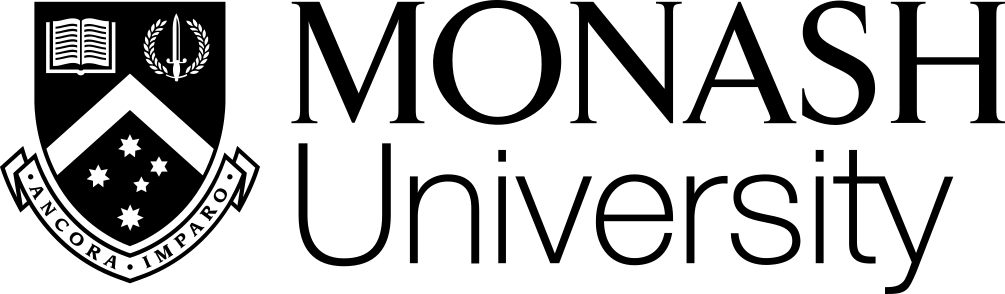
\includegraphics[scale=0.4]{monash_university_logo.png}
        \end{center}
        \vfill

        \textit{Honours \thesis{} in the School of Mathematics, Monash University}
    \end{center}
\end{titlepage}

\chapter*{Abstract}

A \textit{permutation group} $G$ of degree $n$ is a subgroup of the symmetric group $\Sym(\Omega)$ that acts on a set $\Omega$ of size $n$, where $\Sym(\Omega)$ is the group of bijections $\Omega \to \Omega$. An ordered list $B = [\beta_1,\dotsc,\beta_r]$ of distinct elements of $\Omega$ is a \textit{base} for $G$ if the pointwise stabiliser $G_{(B)}$ is trivial; the minimal size of a base for $G$ is denoted $b(G)$. Every base $B = [\beta_1,\dotsc,\beta_r]$ has an associated \textit{stabiliser chain} $G = G^0 \geq G^1 \geq \dotsb \geq G^r = 1$, where each subgroup $G^i = G^{i-1}_{\beta_i}$ in the chain is a stabiliser of the previous subgroup; a \textit{strong generating set} $S$ for $G$ relative to $B$ is a generating set for $G$ such that $G^i = \langle S \cap G^i \rangle$ for each $i$. The combined concept of a \textit{BSGS (base and strong generating set)} allows us to easily perform various computations with permutation groups, such as membership testing and random element generation. In this \thesis{}, we first analyse group actions and bases, and give an introduction to complexity theory. Then, we follow Blaha's proof in \cite{blaha1992} that the \textit{minimum base problem} is NP-hard even if restricted to cyclic groups or elementary abelian group, and discuss a greedy algorithm for computing a small base for $G$, which is not optimal but still useful in practice. Subsequently, we consider various classification results in group theory, such as the \textit{classification of finite simple groups} and the \textit{O'Nan-Scott theorem} for primitive permutation groups, which we use to discuss recent progress in bounding the minimal base size $b(G)$ for groups that are not \textit{large base}: a permutation group $G$ is large base if contains a power of an alternating group, and is itself embedded in a \textit{wreath product} of certain symmetric groups. Finally, we investigate a question from Moscatiello and Roney-Dougal in \cite{moscatiello_roney-dougal2021}, and using computational methods in \texttt{GAP} and the greedy base algorithm, we show that there are very few primitive subgroups $G \leq \Sym(2^d)$, where $1 \leq d \leq 10$, such that $b(G) = d + 1$. These groups are subgroups of the \textit{affine group} $\AGL_d(2)$, and there are none for $d = 1$, one for $d = 2$ and odd $3 \leq d \leq 9$, and two for even $4 \leq d \leq 10$, all up to conjugacy.

\chapter*{Acknowledgements}

Firstly, I would like to express my gratitude to my supervisors Heiko and Santiago, who provided me with guidance and direction. I appreciate their tireless effort in imparting their knowledge, and for the hours spent reading over my \thesis{} to give prompt and useful feedback, even on weekends and late at night. I would also like to thank Norm, Ian, Nick, Wenhui, Andrea, Todd, Jessica, Tim and Eric, whose courses I have learned and received much from, and for the valuable feedback from coursework that has shaped my \thesis{}.

I would also like to thank my friends in the Honours cohort, especially Jeremy, Will and Clayton, for their friendship and support over the year, for all the good memories, and for giving me useful tips for my \thesis{}. For Puti too, who has helped me so much. This extends to various members of online communities -- the Maths @ Monash and Chats \& Reacts Discord servers, whose company I have been blessed with over this year.

I would like to thank my parents for the countless hours they have spent supporting me in every way at home to give me time and energy to maintain my busy schedule. I would also like to thank my friend Wes for being my greatest support through good and trying times this year, and giving me inspiration and assistance for my Honours presentation on the Rubik's group of permutations. Also, to all my church group members and fellow leaders for their constant support and care in busy times.

Lastly, I would like to thank God for His guiding hand in my life, and for being the reason I am where I am today. In the midst of busyness and challenges this year, His presence has given me hope, rest and security. I am so grateful for His constant love, faithfulness, mercy and grace, and I thank Him for this Honours experience in this season of my life:

\begin{quote}
    ``There is a time for everything, \\
    \hspace*{15pt} and a season for every activity under the heavens'' \\
    \null\hfill --- Ecclesiastes 3:1 (NIV)
\end{quote}

\tableofcontents

\chapter{Introduction}

\pagenumbering{arabic}

\section{Assumed knowledge}

This \thesis{} will assume knowledge of content covered in the (former) undergraduate unit MTH3121 -- Algebra and number theory I, run at Monash University until 2021, in particular the group theory half of the unit. It covers basic group theoretic concepts, such as isomorphism, homomorphisms, subgroups, cosets, Lagrange's theorem (see appendix), normal subgroups, quotient groups, and the first isomorphism theorem (see appendix), and studies cyclic groups, dihedral groups, symmetric groups and alternating groups. It did not cover group actions, bases, and related topics, which are therefore included here in the following chapters.

\section{Motivation}

Traditionally, a major goal of research in algebra has been to answer, in various ways, the question of finding all the algebraic structures that satisfy particular axioms, as noted in \cite{cannon_havas1992}. One such major result in this area was the famous classification of finite simple groups, which are finite groups whose only normal subgroups are the trivial ones. In \cite{solomon2001}, it is noted that around the year 2000, computational methods for groups were useful in calculating and classifying finite groups of various orders. This has all stemmed from the development of computational methods in algebra, especially in group theory, since the early 1970s, to compute information about groups for various purposes. In \cite{cannon_havas1992}, Cannon and Havas note that the state of development of computational group theory is relatively advanced, and has seen applications not only in the study of groups, but also in many other branches of mathematics which use group theoretic methods, for example differential equations, graph theory, number theory and topology.

Cannon and Havas observe in \cite{cannon_havas1992} that the study of permutation groups is one of the areas in computational group theory that has traditionally seen high activity. A permutation group is a subgroup of the symmetric group $\Sym(\Omega)$ on some set $\Omega \neq \emptyset$, which is the group of all bijections $\Omega \to \Omega$ under composition. Permutation groups are particularly nice to work with computationally, as their elements can be explicitly identified as permutations on a set, and computations in the group can be easily performed by composing these permutations, say by a computer. Various computational packages such as \texttt{GAP} have been developed, which have implemented permutation groups computationally. Solomon observes in \cite{solomon2001} that computational methods for permutation groups have been considered in the classification problem for finite simple groups, among other applications. Every finite group can be represented as a permutation group by Cayley's theorem, and the degree (size of the set being permuted) of a permutation group representation is often small, \added{4}{especially compared to the size of the group.}

Let $G \leq \Sym(\Omega)$ be a permutation group. To study $G$, the notion of group actions is particularly useful, since elements of $G$ are permutations of $\Omega$, so $G$ acts naturally on $\Omega$ by permutation. This also allows us to explore the notion of bases and stabiliser chains: a base $B$ is a list of elements of $\Omega$ such that the identity $1_{\Sym(\Omega)}$ is the only permutation that fixes each element in $B$, and a stabiliser chain \added{4}{(as introduced and \added{4}{implemented} by Sims in \cite{sims1970})} is a subgroup series, with each group in the series being the stabiliser of a base element in the preceding group. \added{2}{(See section \ref{sec:bases_stabiliser_chains} for details and examples.)} These notions allow us to answer a few natural questions about permutation groups, in particular \added{2}{determining} the order of $G$, finding a generating set for $G$ when realised as a group of permutations of certain objects (for example, vertices of an $n$-gon and vertices in a graph), \added{2}{determining} membership of arbitrary permutations $g \in \Sym(\Omega)$ in the subgroup $G$, and generating random elements of $G$. These preliminary questions are illustrated and addressed in this \thesis{}.

Bases and stabiliser chains have been \added{2}{an} instrumental tool in developing group theoretic algorithms, and effectively facilitate the storing and analysing of large permutation groups. Given the notion of bases and stabiliser chains, it is natural to ask about the possible sizes of a base, and if there are bounds on the size, perhaps if there is an efficient way to find a minimum (smallest) base. For instance, it can be easily seen that for $G = \Sym(n)$ the symmetric group on $n$ elements $\Omega = \{1,\dotsc,n\}$, a minimum base has size $b(G) = n-1$. However, \added{4}{a natural permutation representation of a dihedral group $G = D_{2n}$ (that also acts on $\Omega$) has minimum base size 2}. Since every element in a permutation group is completely determined by its action on a base, a small base can reduce the space required to store the group.

In \cite{blaha1992}, Blaha discusses the question of whether a polynomial time greedy algorithm suggested in \cite{brown1989} always finds a minimum base for a permutation group $G$, to answer the question ``for what $r$ does a permutation group $G$ have a base of size at most $r$?'' He shows that this is not the case, and even when restricted to elementary abelian groups, the problem is NP-hard. \added{2}{However}, Blaha shows that the algorithm presented produces a base of size $O(\mathcal{M}(G)\log\log n)$ where $\mathcal{M}(G)$ is the size of a minimum base for $G \leq \Sym(n)$, and that in the worst case, this bound, \added{2}{which is strictly larger than $\mathcal{M}(G)$,} is actually attained. \added{4}{(Note that all logarithms are base 2.)}

\added{4}{Another problem that has traditionally attracted much attention was bounding the order of a finite primitive (permutation) group of degree $n$, i.e. a permutation group on $\Omega$ whose natural action is transitive and such that no nontrivial partition of $\Omega$ is preserved by the action \cite{moscatiello_roney-dougal2021}. Since $|G| \leq n^{b(G)}$ (see \autoref{lem:blaha_nonredundant_size}), we can find upper bounds on $|G|$ by finding upper bounds on $b(G)$. In 1889, Bochert proved in \cite{bochert1889} that for a primitive group $G$ of degree $n$ not containing the alternating group $\Alt(n)$, then $b(G) \leq n/2$; \cite{moscatiello_roney-dougal2021} notes that this was one of the first results in this direction.

    In 1984, Liebeck proved in \cite{liebeck1984} that if $G$ is a primitive group of degree $n$ that is not ``large base'' (in the sense of containing a power of an alternating group as a subgroup), then $b(G) < 9\log n$. The result was proven in context improving lower bounds on $\mu(G)$, the minimal degree of $G$, which is the smallest number of points moved by any non-identity element in $G$. This proof utilised the O'Nan-Scott theorem, which classifies primitive groups according to the structures of their \textit{socles}, and also the classification of finite simple groups (which was recently completed at the time), and was able to achieve a much tighter lower bound of $\mu(G) > n/(9 \log n)$ than the best result that was previously available, which was $\mu(G) > (1/2)(\sqrt{n} - 1)$ and due to Babai in \cite{babai1981}.

    In 2021, building on more recent results, Moscatiello and Roney-Dougal proved in \cite{moscatiello_roney-dougal2021} that if $G$ is a primitive group of degree $n$ that is not large base, then either $G$ is the Mathieu group $M_{24}$, or $b(G) \leq \lceil\log n\rceil + 1$; moreover, there are infinitely many groups for which $b(G) > \log n + 1$. The Mathieu group $M_{24}$ is a member of the first family of sporadic simple groups discovered as part of the classification of finite simple groups, which are 26 finite simple groups that do not fit into the three infinite families (cyclic, alternating, Lie type).

    The authors of \cite{moscatiello_roney-dougal2021} then present a question, which asks to identify primitive groups $G$ of degree $n$ that satisfy $b(G) = \log n + 1$. They note that $G$ must be a subgroup of the affine group $\AGL_d(2)$ of affine transformations of $\F_2^d$ for some $d$, and that if $d$ is even then groups such as the split extension $2^d : \Sp(d,2)$ have this property. Upon investigation using a recursive approach for $d \leq 10$, we found that apart from the affine group $\AGL_d(2)$, there were no other primitive groups for odd $d$, and for even $d$, the only other example found was $2^d : \Sp(d,2)$. Consequently, we conjecture in this \thesis{} that these are the only groups satisfying this property. Limitations of this approach include memory and computational time, since the group found for $d = 10$ has order $25\,410\,822\,678\,459\,187\,200 \approx 2.5 \cdot 10^{19}$ and thus has many subgroups.}

This \thesis{} largely builds up to a discussion of the results about the NP-hardness of the minimum base problem in \cite{blaha1992}. Firstly, a detailed introduction to group-theoretic concepts such as group actions, bases and stabiliser chains is presented. Then, necessary concepts from complexity theory are introduced. Next, a detailed discussion of \cite{blaha1992} expands on Blaha's proof \added{4}{that finding a minimum base is NP-hard (even for groups with bounded orbits), and summarises the results on sharp bounds for nonredundant and greedy bases. Afterwards, we review classification results for permutation groups, including the classification of finite simple groups, semidirect and wreath products, affine groups, and the influential O'Nan-Scott theorem for primitive groups. Finally, we discuss improvements in bounds on $b(G)$ for non-large-base primitive groups $G$ as found by Liebeck in \cite{liebeck1984} and Moscatiello and Roney-Dougal in \cite{moscatiello_roney-dougal2021}, and investigate the question posed on primitive groups of degree $n$ that satisfy $b(G) = \log n + 1$. Future directions include more investigation into the question from \cite{moscatiello_roney-dougal2021} and the conjecture presented in this \thesis{}, collecting various known results and bounds for base sizes of large-base primitive groups and imprimitive permutation groups, and identifying special classes of examples where specific bounds or results can be newly found in relation to the NP-hardness of the minimum base problem and analysis of the greedy base algorithm.}

% \begin{itemize}
%     \item What is the problem
%     \item Overview of CGT
%     \item Why are minimum bases desirable
%     \item Tradeoffs with size of transversals?
%     \item Blaha's paper
%     \item Recent advances; what is known
%     \item List notation (where?)
%     \item Emphasise that chapters 2 \& 3 are new?
% \end{itemize}

\chapter{Preliminary concepts from permutation groups}

\added{1}{Permutation groups, which are groups whose elements are realised as permutations of some (nonempty) set $\Omega$, play a central role in \textbf{computational group theory}, which uses computational methods to compute and store information about groups. The notion of a \textit{group action} arises naturally from the concept of permutation groups, since group actions encode group elements as permutations: every permutation group on $\Omega$ naturally induces an action on $\Omega$, and a permutation group arises from every group action. Let $G$ be a group and $\alpha \in \Omega$; the notions of an \textit{orbit} and \textit{stabiliser} of $\alpha$ can be defined for $G$-actions on $\Omega$. \added{2}{(The stabiliser of $\alpha$ comprises elements $g \in G$ whose associated permutations fix $\alpha$.)} A \textit{base} is an ordered list $B$ of elements of $\Omega$ such that only the identity element $1 \in G$ fixes every element of $B$ pointwise; a base gives rise naturally to a series of stabiliser subgroups called the \textit{stabiliser chain}, and a generating set that respects this structure is called a \textit{strong generating set}; these are used in numerous algorithms across computational group theory. We now approach this formally.}

\added{1}{
    \begin{definition}\label{def:permutation_group}
        Let $\Omega$ be a set. The \textbf{symmetric group} $\Sym(\Omega)$ on $\Omega$ consists of \textit{permutations} of $\Omega$ (bijections $\Omega \to \Omega$) under composition. A \textbf{permutation group} on $\Omega$ is a subgroup of $\Sym(\Omega)$; its \textbf{degree} is $|\Omega|$.
    \end{definition}}

\added{1}{When $\Omega = [n] := \{1,\dotsc,n\}$, we instead write $\Sym(n)$ for the \textit{symmetric group} of degree $n$.} \added{3}{(A similar notation is $\Alt(n)$ for the \textit{alternating group} of degree $n$ of even permutations of $n$.)} In this \thesis{}, we use the following conventions: for $\alpha \in \Omega$ and $g,h \in \Sym(\Omega)$, write $\alpha^g$ for the image of $\alpha$ under $g$ (instead of $g(\alpha)$ or $g \alpha$), and we perform $g$ then $h$ in the composition (product) $gh$, so that $\alpha^{gh} = (\alpha^g)^h$. \added{1}{Also, for the trivial subgroup we write $1 = \{1\} \leq G$.}

As permutations are a central object of study, we recall \added{1}{the} \textit{disjoint cycle notation}. Let $\Omega$ be a set; if $\alpha_1,\dotsc,\alpha_r$ are distinct elements of $\Omega$, we write $\sigma = (\alpha_1,\alpha_2,\dotsc,\alpha_r)$ for the cycle $\sigma \in \Sym(\Omega)$ with $\alpha_i^\sigma = \alpha_{i+1}$ for $1 \leq i < r$, $\alpha_r^\sigma = \alpha_1$, and $\alpha^\sigma = \alpha$ for $\alpha \in \Omega \setminus \{\alpha_1,\dotsc,\alpha_r\}$. If $\Omega$ is finite, then every permutation can be decomposed into a product of disjoint cycles; we generally omit fixed points (cycles of length 1). \added{1}{The lengths of these cycles give the \textit{cycle type} of $\sigma$. The identity permutation $\Id_\Omega$ is written as $1_{\Sym(\Omega)}$, $()$, or just $1$ when context is clear.}

\added{3}{A group $G$ is \textbf{generated by a set} $X$ if every $g \in G$ can be written as} $g = x_1^{\varepsilon_1}\dotsb x_k^{\varepsilon_k}$ with each $x_i \in X$, $\varepsilon_i = \pm 1$, and $k \in \N$; if $k = 0$ then we have the empty product $g = 1$. We write $G = \langle X \rangle$. When \added{2}{$G = \langle X \rangle$ for some finite $X$}, $G$ is \textbf{finitely generated}. \added{3}{When $X,Y \subseteq G$, we write $\langle X,Y \rangle = \langle X \cup Y \rangle \leq G$ as the subgroup generated by $X$ and $Y$; this notion naturally extends to any finite number of subsets of $G$.}

% A \textbf{group presentation} of a group $G$ is a nonempty set $X$ of \textbf{generators} and a set $R$ of \textbf{relations} such that $G = \langle X \rangle$ and $R$ is a subset of the free group $F_X$ on $X$ such that for any relator $r \in R$, $r = 1$ in $G$, and we can write $r = y_1^{\varepsilon_1}\dotsb y_\ell^{\varepsilon_\ell}$ with $\ell \in \N$ and each $y_i \in X$ and $\varepsilon_i = \pm 1$. We write $G = \langle X \mid R \rangle$; we can see that $G$ is isomorphic to a quotient of the free group $F_X$ by the smallest normal subgroup containing $R$.

\section{Group actions}

\added{3}{The following section is largely adapted from Holt \cite{holt_handbook_cgt2005}, \added{4}{with original examples and illustrations}.}

We often think of $D_{2n}$, the dihedral group of order $2n$, as the \added{2}{symmetry} group of a regular $n$-gon. But abstractly, \mbox{$D_{2n} = \langle r,s \mid r^n,s^2,srsr \rangle$} is defined by a presentation, a set of generators and relations. The precise way in which elements of $D_{2n}$ ``are'' symmetries is given by an \textit{action} of $D_{2n}$ on say the \added{1}{vertex set} $\Omega$ of a regular $n$-gon; each element of $D_{2n}$ permutes $\Omega$, and the product in $D_{2n}$ mirrors compositions of corresponding permutations. The following definition formalises this idea and extends it to other groups.

\begin{definition}\label{def:action}
    Let $G$ be a group and $\Omega \neq \emptyset$ be a set. A \textbf{(group) action} of $G$ on $\Omega$ is a homomorphism $G \to \Sym(\Omega)$. \added{3}{The \textbf{degree} of the action is $|\Omega|$.}
\end{definition}

If we have an action, we say that $G$ \textit{acts} on $\Omega$. Immediately, we see that the image of an action is a permutation group; an action gives a way of describing how a group $G$ permutes a set $\Omega$ in a way that respects the structure of $G$. If $\varphi$ is an action as defined above, then $\varphi(g)$ is a permutation of \added{4}{$\Omega$} for each $g \in G$. If $\varphi$ is fixed \added{4}{or implied}, we usually write $\alpha^g := \alpha^{\varphi(g)}$ for the action of $\varphi(g)$ on $\alpha \in \Omega$. (Implicit in this notation is that we think of $g \in G$ as acting on elements of $\Omega$ from the right.) \added{4}{When we omit the action $\varphi$, its image $\varphi[G]$} is denoted $G^\Omega$, which is a \textit{permutation group} on $\Omega$. \added{2}{By the \hyperref[thm:FIT]{first isomorphism theorem}, $\varphi[G] \cong G/\ker\varphi$ is isomorphic to a quotient of $G$.}

Note that since $\varphi$ is a homomorphism, this translates to the property that
$$\alpha^{gh} = \alpha^{\varphi(gh)} = \alpha^{\varphi(g)\varphi(h)} = (\alpha^{\varphi(g)})^{\varphi(h)} = (\alpha^g)^h$$
for $g,h \in G$ and $\alpha \in \Omega$. Also, since $\varphi(1) = 1_{\Sym(\Omega)} = \Id_\Omega$, we see that $\alpha^1 = \alpha$ for $\alpha \in \Omega$. Indeed, one can verify that these two properties characterise actions of $G$ on $\Omega$.

\begin{lemma}\label{lem:verify_action}
    The map $\varphi : G \to \Sym(\Omega)$ is an action of $G$ on $\Omega$ if and only if (1), $\alpha^1 = \alpha$ and (2), $\alpha^{gh} = (\alpha^g)^h$ for all $g,h \in G$ and $\alpha \in \Omega$. \added{2}{(Recall the convention $\alpha^g := \alpha^{\varphi(g)}$.)} \qedhere
\end{lemma}

Another useful property of actions is that if $\alpha^g = \beta$ for $g \in G$ and $\alpha,\beta \in \Omega$, then $\beta^{g^{-1}} = \alpha$; this follows from the fact that $\varphi(g^{-1}) = \varphi(g)^{-1}$ \added{4}{for the group homomorphism $\varphi$}. We now provide some examples of actions on groups.

\added{1}{\begin{example}[trivial action]\label{eg:trivial_action}
        An element $g \in G$ \textbf{acts trivially} (on $\Omega$) if $\alpha^g = \alpha$ for all $\alpha \in \Omega$, i.e. $g \mapsto 1 \in \Sym(\Omega)$. If every $g \in G$ acts trivially, then we have the \textbf{trivial action} on $G$, and we say that $G$ \textbf{acts trivially} on $\Omega$.
    \end{example}}

\begin{example}[right regular action]\label{eg:right_regular_action}
    Let $G$ be a group and $\Omega = G$, the underlying set of $G$. Let $g \in G$ act on $\alpha \in G$ (via $\mathcal{R} : G \to \Sym(G)$) by $\alpha^g := \alpha g$. Then $\mathcal{R}$ is an action by \autoref{lem:verify_action}: (1), we have $\alpha^1 = \alpha 1 = \alpha$ for $\alpha \in G$; and (2), for $g,h \in G$ and $\alpha \in G$, $\alpha^{gh} = \alpha gh = (\alpha g)h = (\alpha^g)^h$, so that $\mathcal{R}(gh) = \mathcal{R}(g)\mathcal{R}(h)$. This is the \textbf{right regular action} $\mathcal{R}$ on $G$; \added{1}{here} $G$ acts on itself by right-multiplication. \added{1}{The image $G^\Omega = \mathcal{R}[G] \leq \Sym(G)$ is the \textbf{right regular \added{3}{permutation} representation} of $G$.}
\end{example}

\added{1}{\begin{example}[representations]\label{eg:representations}
        Let $G$ be a group and $\Omega = V$, a $K$-vector space \added{4}{with $K$ a field}. Let $\rho : G \to \Sym(V)$ be a homomorphism with $\rho[G] \leq \GL(V) = \Aut(V)$, the invertible linear maps $V \to V$. Then $\rho$ is an action \added{2}{of $G$ on $V$}, but we typically write $\rho : G \to \GL(V)$ and call it a \textbf{representation} of $G$; these are studied in a branch of mathematics called representation theory, which \added{2}{analyses $G$ using} linear actions on a vector space, whose properties are well-known.
    \end{example}}

There is a natural notion of equivalence of actions \added{2}{on a fixed group $G$}.

\begin{definition}\label{def:equivalent_action}
    Two \textit{actions} $\varphi,\tilde\varphi$ of $G$ on $\Omega,\tilde\Omega$ are \textbf{equivalent} if there is a bijection $\tau : \Omega \to \tilde\Omega$ \added{2}{such that $\tau(\alpha^{\varphi(g)}) = \tau(\alpha)^{\tilde\varphi(g)}$ (or equivalently, $\tau(\alpha^g) = \tau(\alpha)^g$)} for all $g \in G$ and $\alpha \in \Omega$.
\end{definition}

\added{2}{This notion of equivalence says that applying $\varphi$ then relabelling $\Omega$ via $\tau$ is the same as relabelling $\Omega$ via $\tau$ then applying $\tilde\varphi$. In other words, the following diagram commutes \added{4}{for all $g \in G$}:}

% https://q.uiver.app/?q=WzAsNCxbMCwwLCJcXE9tZWdhXzEiXSxbMCwyLCJcXE9tZWdhXzIiXSxbMiwwLCJcXE9tZWdhXzEiXSxbMiwyLCJcXE9tZWdhXzIiXSxbMCwxLCJcXHRhdSJdLFsyLDMsIlxcdGF1IiwyXSxbMSwzLCJcXHZhcnBoaV8yKGcpIl0sWzAsMiwiXFx2YXJwaGlfMShnKSIsMl1d
\[\begin{tikzcd}
        {\Omega} && {\Omega} \\
        \\
        {\tilde\Omega} && {\tilde\Omega}
        \arrow["\tau", from=1-1, to=3-1]
        \arrow["\tau"', from=1-3, to=3-3]
        \arrow["{\tilde\varphi(g)}", from=3-1, to=3-3]
        \arrow["{\varphi(g)}"', from=1-1, to=1-3]
    \end{tikzcd}\]

\added{2}{There is a similar notion of isomorphic permutation groups, where the natural action is preserved:

    \begin{definition}\label{def:permutation_equivalent}
        Two permutation groups $G \leq \Sym(\Omega)$ and $H \leq \Sym(\tilde\Omega)$ are \textbf{permutation isomorphic} if there is a bijection $\tau : \Omega \to \tilde\Omega$ and an isomorphism $\psi : G \to H$ such that $\tau(\alpha^g) = \tau(\alpha)^{\psi(g)}$ for all $g \in G$ and $\alpha \in \Omega$.
    \end{definition}

    The condition on $\tau,\psi$ says that the following diagram commutes \added{4}{for all $g \in G$}:}

% https://q.uiver.app/?q=WzAsNCxbMCwwLCJcXE9tZWdhXzEiXSxbMCwyLCJcXE9tZWdhXzIiXSxbMiwwLCJcXE9tZWdhXzEiXSxbMiwyLCJcXE9tZWdhXzIiXSxbMCwxLCJcXHRhdSJdLFsyLDMsIlxcdGF1IiwyXSxbMSwzLCJcXHBzaShnKSBcXGluIEgiXSxbMCwyLCJnIFxcaW4gRyIsMl1d
\[\begin{tikzcd}
        {\Omega} && {\Omega} \\
        \\
        {\tilde\Omega} && {\tilde\Omega}
        \arrow["\tau", from=1-1, to=3-1]
        \arrow["\tau"', from=1-3, to=3-3]
        \arrow["{\psi(g) \in H}", from=3-1, to=3-3]
        \arrow["{g \in G}"', from=1-1, to=1-3]
    \end{tikzcd}\]

\added{3}{In the special case that $G = H$ and $\psi = \Id_G$, then permutation isomorphism yields equivalence: for $g \in G$ and $\alpha \in \Omega$, since $G,H$ are permutation isomorphic, we have $\tau(\alpha^g) = \tau(\alpha)^{\Id_G(g)} = \tau(\alpha)^g$ \added{4}{for all $g \in G$}, so the actions are equivalent via $\tau$.}

Next, we define what it means for an action to be \textit{faithful}.

\begin{definition}\label{def:faithful_action}
    An \textit{action} $\varphi$ of $G$ on $\Omega$ is \textbf{faithful} if $\ker\varphi = 1$. In other words, if $\alpha^g = \alpha$ for all $\alpha \in \Omega$, then $g = 1$.
\end{definition}

If $\varphi$ is faithful, then $1$ is the only element of $G$ that does not permute any elements in $\Omega$. This also says that $G$ embeds into $\Sym(\Omega)$ via $\varphi$: $G \cong G/1 = G/\ker\varphi \cong \added{1}{G^\Omega}$ by the \added{1}{\hyperref[thm:FIT]{first isomorphism theorem}}. A natural question arises: is there a faithful action for any group $G$? If this were true, then every group would be isomorphic to a permutation group. This is answered in the affirmative by Cayley's theorem, which is part of Fact 2 in \cite{blaha1992}.

\begin{theorem}[Cayley]\label{thm:cayley}
    Let $G$ be a group and $\mathcal{R}$ be the right regular action of $G$. Then $G$ is isomorphic to the permutation group $\mathcal{R}[G] \leq \Sym(G)$. In the case that $|G| = n$ is finite, then $G$ is isomorphic to a subgroup of $\Sym(n)$.
\end{theorem}

\begin{proof}
    Recall the right regular action $\mathcal{R}$ as defined in \autoref{eg:right_regular_action}. From above, it suffices to show that $\mathcal{R}$ is faithful: let $\alpha \in G$ and suppose $\alpha^g = \alpha$. Then $\alpha g = \alpha$, so \added{1}{left multiplication by $\alpha^{-1}$ gives} $g = 1$, as required.
\end{proof}

\begin{example}[natural action]\label{eg:natural_action}
    Let $G \leq \Sym(\Omega)$ be a permutation group. The \textbf{natural action} $\varphi : G \to \Sym(\Omega)$ of $G$ on $\Omega$ is given by the inclusion map $g \mapsto g$ (so that for $\alpha \in \Omega$ \added{4}{and $g \in G$}, $\added{4}{\alpha^{\varphi(g)}} := \alpha^g$, the image of $\alpha$ under $g$); this is faithful. (Note that the image $G^\Omega \leq \Sym(\Omega)$ of an arbitrary $G$-action on $\Omega$ takes the natural action; it yields a homomorphism $G \to G^\Omega$, and $G^\Omega$ is a \textit{homomorphic image} of $G$ that acts faithfully on $\Omega$.)
\end{example}

\begin{example}[quotient action]\label{eg:quotient_action}
    Let $G$ act on $\Omega$ via $\varphi$. If $N \unlhd G$ is contained in $\Ker\varphi$, then the quotient group $G/N$ acts on $\Omega$ by $\alpha^{gN} := \alpha^g$ for $\alpha \in \Omega$ and $gN \in G/N$. This is well-defined: if $\alpha \in \Omega$ and $gN = hN$ then $gh^{-1} \in N$ (since $N$ is normal in $G$), so $gh^{-1} \in \ker\varphi$, so $\alpha^{gh^{-1}} = \alpha$, which implies $\alpha^g = \alpha^h$. Also, we verify that $\alpha^{1_{G/N}} = \alpha^{1N} = \alpha^1 = \alpha$ and $(\alpha^{gN})^{hN} = (\alpha^g)^h = \alpha^{gh} = \alpha^{ghN} = \alpha^{(gN)(hN)}$ for $\alpha \in \Omega$ and $gN,hN \in G/N$.

    Note that the $G/N$-action $\hat\varphi$ on $\Omega$ is faithful if and only if $N = \Ker\varphi$. This is because
    $$\Ker\hat\varphi = \{gN \in G/N : \alpha^{gN} = \alpha^g = \alpha\ \text{for all}\ \alpha \in \Omega\} = \{gN \in G/N : g \in \Ker\varphi\} = \Ker\varphi/N,$$
    and $\Ker\varphi/N = 1$ if and only if $N = \Ker\varphi$. (Then if $K = \Ker\varphi$, then $G/K$ and $G^\Omega \leq \Sym(\Omega)$ are permutation isomorphic, via the identity relabelling $\tau : \Omega \to \Omega$ and the natural isomorphism $\psi : G/K \to G^\Omega$ (see \autoref{thm:FIT}), $gK \mapsto \varphi(g)$, since for $\alpha \in \Omega$ and $gK \in G/K$, we have $\tau(\alpha^{gK}) = \alpha^{gK} = \alpha^{\varphi(g)} = \tau(\alpha)^{\psi(gK)}$.)
\end{example}

% If $G \leq \Sym(\Omega)$ is a permutation group that acts on $\tilde\Omega$ via $\varphi : G \to \Sym(\tilde\Omega)$ that is not the natural action, then $\varphi$ may not be faithful. However, the above shows that $G/\Ker\varphi$ acts faithfully on $\tilde\Omega$. By the first isomorphism theorem, $G/\Ker\varphi$ is isomorphic to a subgroup of $\Sym(\tilde\Omega)$, so we may identify $G/\Ker\varphi$ as a permutation group on $\tilde\Omega$, where the action is induced by $\varphi$. % (This is useful in the analysis of certain permutation groups such as the Rubik's group.)

\begin{example}\label{eg:action_D8_on_square}
    Consider $D_8 = \{1,r,r^2,r^3,s,\added{2}{sr,sr^2,sr^3}\}$, the dihedral group of order 8. It ``is'' the \added{2}{symmetry} group of a square $S$ (with vertices $V = \{v_1,v_2,v_3,v_4\}$ labelled anticlockwise) in the following sense: let $r \mapsto (v_1,v_2,v_3,v_4)$ and $s \mapsto (v_1,v_4)(v_2,v_3)$ generate the (faithful) action of $D_8$ on $V$. For example, $v_4^{rs} = (v_4^r)^s = v_1^s = v_4$. \added{1}{By renaming elements of $V$, we see that this is equivalent} to the action of $D_8$ on the set $\{1,2,3,4\}$ defined by $r \mapsto (1,2,3,4)$ and $s \mapsto (1,4)(2,3)$, so we see that \added{1}{$D_8$ is isomorphic to a subgroup of $\Sym(4)$}.

    Now let $D = \{d_1,d_2\}$ be the set of diagonals of $S$, where $d_1$ joins $v_1$ and $v_3$, and $d_2$ joins $v_2$ and $v_4$. A corresponding action $\varphi$ of $D_8$ on $D$ is given by $\varphi(r) = \varphi(s) = (d_1,d_2)$: for example, $d_1^{rs} = (d_1^r)^s = d_2^s = d_1$. Then the kernel of $\varphi$ is $\{1,r^2,\added{2}{sr,sr^3}\} \trianglelefteq D_8$; the action is not faithful.

    Now consider the corresponding action of $D_8$ on $\Omega = \{S,v\}$, where $v$ is the centre of $S$. Every \added{2}{symmetry} of $S$ fixes $S$ and its centre, so $S^g = S$ and $v^g = v$ for all $g \in D_8$, so $D_8$ acts trivially on $\Omega$.
\end{example}

\subsection{Orbits and stabilisers}

We define orbits, stabilisers and fixed point sets for an action of $G$ on $\Omega$, which are fundamental to the study of actions.

\begin{definition}\label{def:orbit_stabiliser}
    Let $G$ act on $\Omega$.
    \begin{enumerate}[(i)]
        \item The \textbf{orbit} of $\alpha \in \Omega$ is $\alpha^G = \{\alpha^g : g \in G\} \subseteq \Omega$.
        \item \added{3}{The \textbf{pointwise stabiliser} of $\Delta \subseteq \Omega$ is $G_{(\Delta)} = \{g \in G : \alpha^g = \alpha\ \text{for all}\ \alpha \in \Delta\} \subseteq G$.}
        \item The \textbf{fixed point set} of $g \in G$ is $\Fix_\Omega(g) = \{\alpha \in \Omega : \alpha^g = \alpha\} \subseteq \Omega$, dually to the stabiliser.
    \end{enumerate}
\end{definition}

\added{3}{In (ii) above, if $\Delta = \{\alpha\}$ then we write $G_\alpha = \{g \in G : \alpha^g = \alpha\} \subseteq G$ for the \textbf{(point) stabiliser} of $\alpha \in \Omega$. If $\Delta = \{\alpha_1,\dotsc,\alpha_k\}$, then we may write $G_{(\Delta)} = G_{\alpha_1,\dotsc,\alpha_k}$. For $\alpha \in \Delta$, it is often useful to note that $G_{(\Delta)} = (G_{(\Delta \setminus \alpha)})_{\alpha}$. The stabiliser of an element of $\Omega$ is a \textit{subgroup} of $G$:}

\begin{proposition}\label{prop:stabiliser_subgroup}
    Let $G$ act on $\Omega$ and $\alpha \in \Omega$. Then $\added{2}{G_\alpha} \leq G$.
\end{proposition}

\begin{proof}
    \added{2}{We use the subgroup criterion.} First $1 \in \added{2}{G_\alpha}$, since $\alpha^1 = \alpha$. Let $g,h \in \added{2}{G_\alpha}$; then
    $$\alpha^{gh^{-1}} = (\alpha^g)^{h^{-1}} = \alpha^{h^{-1}} = \alpha,$$
    so $gh^{-1} \in \added{2}{G_\alpha}$. \added{1}{The third equality follows from applying $h^{-1}$ to the equality $\alpha^h = \alpha$.}
\end{proof}

\added{2}{Since the intersection of subgroups is a subgroup and $G_{(\Delta)} = \bigcap_{\alpha \in \Delta} G_\alpha$, we get the following:

    \begin{corollary}\label{cor:pointwise_stabiliser_subgroup}
        Let $G$ act on $\Omega$ and $\Delta \subseteq \Omega$. Then $G_{(\Delta)} \leq G$. \qedhere
    \end{corollary}}

\begin{proposition}\label{prop:kernel_action_stabiliser}
    Let $G$ act on $\Omega$. Then the kernel of the action is $\added{2}{G_{(\Omega)}} = \bigcap_{\alpha \in \Omega} \added{2}{G_\alpha} \trianglelefteq G$.
\end{proposition}

\begin{proof}
    Let $K$ be the kernel, which contains the elements of $G$ which map to $\Id_\Omega$ under the action. \added{2}{Then $g \in K$ if and only if $\alpha^g = \alpha$ for all $\alpha \in \Omega$, so $K = G_{(\Omega)}$. The result then follows from \autoref{cor:pointwise_stabiliser_subgroup}.}
\end{proof}

The orbits of $G$ on $\Omega$ partition $\Omega$: indeed, if we define a relation on $\Omega$ by saying $\alpha,\beta \in \Omega$ are related when some orbit contains both $\alpha$ and $\beta$, this is an equivalence relation, and the orbits are the equivalence classes.

\begin{example}\label{eg:rra_orbits_stabilisers}
    \begin{enumerate}[(a)]
        \item Recall the right regular action $\mathcal{R}$ on $G$ from \autoref{eg:right_regular_action}, and let $\alpha \in G$. Then the orbit of $\alpha$ is $\alpha^G = \{\alpha^g = \alpha g : g \in G\} = G$. The stabiliser of $\alpha$ is $\added{2}{G_\alpha} = \{g \in G : \alpha g = \alpha^g = \alpha\} = 1$. The fixed point set of $g \in G$ is $\Fix_G(g) = \{\alpha \in G : \alpha g = \alpha^g = \alpha\}$; this is all of $G$ if $g = 1$, and empty otherwise. Note that if $G$ is finite, we see that $|\alpha^G| |\added{2}{G_\alpha}| = |G| |1| = |G|$.
        \item \added{1}{When $G \leq K$, we can extend $\mathcal{R}$ to a $G$-action $\mathcal{R}^K : G \to \Sym(K)$ on $K$, by $\alpha^g = \alpha g$ for $\alpha \in K$ and $g \in G$. Then the orbits are the left cosets $\alpha G$ of $G$ in $K$, so by \hyperref[thm:lagrange]{Lagrange's theorem}, there are $|K : G|$ orbits, each with size \added{4}{$|G|$}.}
    \end{enumerate}
\end{example}

\begin{example}\label{eg:D8_diagonals_orbits_stabilisers}
    Recall from \autoref{eg:action_D8_on_square} the action $\varphi$ of $D_8$ on $D = \{d_1,d_2\}$, the set of diagonals of a square $S$. The orbit of $d_1$ is $d_1^{D_8} = \{d_1,d_2\} = D$ since $d_1^1 = d_1$ and $d_1^r = d_2$. The stabiliser of $d_1$ is $(D_8)_{d_1} = \{1,r^2,\added{2}{sr,sr^3}\}$. From this, we see that $|d_1^{D_8}| |(D_8)_{d_1}| = 2 \cdot 4 = 8 = |D_8|$. Note that the fixed point sets of $g = 1,r^2,\added{2}{sr,sr^3}$ are all of $D$, but the fixed point sets of $g = r,r^3,s,\added{2}{sr^2}$ are empty.
\end{example}

Since $\added{2}{G_\alpha}$ is a subgroup of $G$, we can consider its (right) cosets. Let $\added{2}{G_\alpha} \backslash G$ denote the set of its right cosets in $G$. From the previous examples, we see a pattern that for any $\alpha \in \Omega$, we have $|G| = |\alpha^G| |\added{2}{G_\alpha}|$, at least when $G$ is finite. This is made precise for any group $G$, possibly infinite, by the \textit{orbit-stabiliser theorem}, which gives a bijection of $\added{2}{G_\alpha} \backslash G$ with the orbit of $\alpha$, i.e. a bijective correspondence between (right) cosets of the stabiliser of $\alpha$ and elements in the orbit of $\alpha$:

\begin{theorem}[orbit-stabiliser (OST); \added{1}{Fact 1 in \cite{blaha1992}}]\label{thm:orbit_stabiliser}
    \added{4}{Let $G$ act on $\Omega$ and let $\alpha \in \Omega$.} The map $\added{2}{G_\alpha} \backslash G \to \alpha^G$ given by $\added{2}{G_\alpha}g \mapsto \alpha^g$ is a bijection. \added{1}{So, the index of $\added{2}{G_\alpha}$ in $G$ is $|G : \added{2}{G_\alpha}| = |\alpha^G|$, and $|G| = |\alpha^G| |\added{2}{G_\alpha}|$ by \hyperref[thm:lagrange]{Lagrange's theorem}.}
\end{theorem}

\begin{proof}
    The map is well-defined, since if $\added{2}{G_\alpha}g = \added{2}{G_\alpha}h$, then $gh^{-1} \in \added{2}{G_\alpha}$, so $\alpha^{gh^{-1}} = \alpha$; applying $h$ results in $\alpha^g = \alpha^{gh^{-1}h} = \alpha^h$, as required. The map is injective: let $g,h \in G$ and suppose $\alpha^g = \alpha^h$. Then $\alpha^{gh^{-1}} = \alpha^1 = \alpha$, so $gh^{-1} \in \added{2}{G_\alpha}$, so $\added{2}{G_\alpha}g = \added{2}{G_\alpha}h$. The map is surjective: let $\alpha^g \in \alpha^G$ where $g \in G$; clearly $\added{2}{G_\alpha}g \mapsto \alpha^g$. So the map is a bijection.
\end{proof}

Note that $\added{2}{G_\alpha}$ may not be a normal subgroup, so we may not be able to talk about quotient groups. But the intersection of stabilisers is normal in $G$ by \autoref{prop:kernel_action_stabiliser}, as the kernel of the action.

\subsection{Conjugacy, centralisers and normalisers}

Another important action of $G$ on $\Omega = G$ is \textit{conjugation}. \added{2}{Recall that an \textbf{automorphism} of $G$ is an isomorphism $G \to G$; the set of automorphisms form a group, $\Aut(G)$, under composition.}

\begin{example}[conjugation]\label{eg:conjugation}
    For $\alpha \in G$, \textbf{conjugation} of $\alpha$ by $g \in G$ gives the element $\alpha^g := g^{-1}\alpha g$. This defines an action of $G$ on $\Omega = G$: $\alpha^1 = 1^{-1}\alpha 1 = \alpha$ and $\alpha^{gh} = (gh)^{-1}\alpha gh = h^{-1}(g^{-1}\alpha g)h = (\alpha^g)^h$ for $\alpha,g,h \in G$.

    The orbit of $\alpha \in G$ is the \textbf{conjugacy class} $\operatorname{Cl}_G(\alpha) := \{g^{-1}\alpha g : g \in G\}$. Elements in the same conjugacy class are said to be \textbf{conjugate} and have the same order, since for $g \in G$ the \textbf{inner automorphism} $G \to G$ given by $\alpha \mapsto g^{-1}\alpha g$ is an automorphism: the inverse map is clearly given by $\alpha \mapsto g\alpha g^{-1}$ (which is conjugation by $g^{-1}$), and we have $g^{-1}\alpha\beta g = (g^{-1}\alpha g)(g^{-1} \beta g)$ for $\alpha,\beta \in G$ (so it is an \textit{endomorphism}). \added{2}{The set of inner automorphisms forms a group, $\Inn(G)$.}

    The stabiliser of $\alpha \in G$ is the \textbf{centraliser} of $\alpha$: suppose $g \in G$ is such that $\alpha^g = g^{-1}\alpha g = \alpha$. Then $\alpha g = g \alpha$, so $\added{2}{G_\alpha} = \{g \in G : \alpha g = g \alpha\} =: C_G(\alpha)$; this is the set of elements that commute with $\alpha$. The \hyperref[thm:orbit_stabiliser]{OST} then implies that $|\operatorname{Cl}_G(\alpha)| = |G|/|C_G(\alpha)|$ \added{1}{in the case that $G$ is finite}. (If $G$ is \textit{abelian}, then $C_G(\alpha) = G$, and it follows that $G$ acts trivially on itself by conjugation.) The kernel of the action is the \textbf{centre} $Z(G) := \{g \in G : \alpha g = g \alpha\ \text{for all}\ \alpha \in G\} \trianglelefteq G$.
\end{example}

We may also define conjugacy and associated notions for subgroups $H$ of $G$; the discussion above then corresponds to the case that $H = 1 \leq G$.

\begin{example}\label{eg:conjugation_subgroups}
    For a \textit{subgroup} $H \leq G$, \textbf{conjugation} of $H$ by $g \in G$ gives the subgroup $H^g = g^{-1}Hg = \{g^{-1}hg : h \in H\} \leq G$. This defines an action of $G$ on the subgroups $\Omega = \{H : H \leq G\}$ of $G$.

    Subgroups in the same orbit are said to be \textbf{conjugate (subgroups)} and are isomorphic: the inner automorphism described in \autoref{eg:conjugation} restricts to an isomorphism $H \to H^g$. However isomorphic subgroups need not be conjugate; if $G$ is abelian, $H^G = \{H\}$ only, and in $G = \Z$ we know that $\Z \cong 2\Z \leq \Z$, for instance. In this context, the orbits are called \textbf{conjugacy classes (of subgroups)}.

    The stabiliser of $H \leq G$ is the \textbf{normaliser} of $H$: suppose $g \in G$ is such that $H^g = g^{-1}H g = H$. Then $Hg = gH$, so $\added{2}{G_H} = \{g \in G : Hg = gH\} =: N_G(H)$; clearly $H \trianglelefteq N_G(H)$, and $N_G(H)$ is the largest subgroup of $G$ with this property. The \hyperref[thm:orbit_stabiliser]{OST} then implies $|G : N_G(H)|$ is the number of subgroups of $G$ conjugate to $H$. The \textbf{centraliser} of $H$ is $C_G(H) = \{g \in G : hg = gh\ \text{for all}\ h \in H\} \subseteq N_G(H)$; we see that $C_G(G) = Z(G)$.
\end{example}

The notion of permutation isomorphism relates to conjugacy of subgroups in a special case.

\added{3}{\begin{lemma}\label{lem:permutation_isomorphism_conjugate_subgrps}
        Let $G,H \leq \Sym(\Omega)$ be permutation isomorphic via $\tau : \Omega \to \Omega$ and $\psi : G \to H$. Then $G$ and $H$ are conjugate subgroups.
    \end{lemma}}

\begin{proof}
    Let $\alpha \in \Omega$ and $g \in G$. Then $H = G^\tau$, where $\tau \in \Sym(\Omega)$: indeed, we have $\psi(g) = \tau^{-1}g\tau$ since
    \[\tau(\alpha)^{\psi(g)} = \tau(\alpha^g) = \alpha^{g\tau} = \tau(\alpha)^{\tau^{-1}g\tau}.\]
\end{proof}

\added{2}{Recall that a \textbf{maximal subgroup} $H$ of $G$ is a subgroup \added{4}{$H < G$} such that $H < K \leq G$ implies $K = G$.

    \begin{lemma}\label{lem:conjugate_of_maximal_subgroup_is_maximal}
        If $H < G$ is maximal, then $H^g$ is maximal for all $g \in G$.
    \end{lemma}

    \begin{proof}
        Suppose for contradiction that $H^g$ is not maximal; then there is $K \leq G$ with $H^g < K < G$. Clearly $K^{g^{-1}} < G$ (since $K \cong K^{g^{-1}}$ by \autoref{eg:conjugation_subgroups}), and moreover for $h \in H$ we have $h = g(g^{-1}hg)g^{-1} \in K^{g^{-1}}$ since $g^{-1}hg \in H^g < K$, so $H < K^{g^{-1}}$. This contradicts maximality of $H$.
    \end{proof}}

There is a useful result that relates the stabilisers of two elements in the same orbit: they are conjugate, thus isomorphic.

\begin{proposition}\label{prop:stabilisers_are_conjugate}
    Let $G$ act on $\Omega$ and let $g \in G$ and $\alpha \in \Omega$. Then $\added{2}{G_{\alpha^g}} = \added{2}{(G_\alpha)}^g$.
\end{proposition}

\begin{proof}
    If $h \in \added{2}{G_{\alpha^g}}$, then $\alpha^{gh} = (\alpha^g)^h = \alpha^g$, so $\alpha^{ghg^{-1}} = \alpha$. Then $h = g^{-1}(ghg^{-1})g \in \added{2}{(G_\alpha)}^g$, since we have $ghg^{-1} \in \added{2}{G_\alpha}$. Conversely, if $h \in \added{2}{(G_\alpha)}^g$, then $h = g^{-1}sg$ for some $s \in \added{2}{G_\alpha}$, so $(\alpha^g)^h = (\alpha^g)^{g^{-1}sg} = \alpha^{sg} = \alpha^g$ since $\alpha^s = \alpha$. So $h \in \added{2}{G_{\alpha^g}}$.
\end{proof}

Recall the condition for equality of right cosets: for $H \leq G$, $Hg = Hk$ if and only if $gk^{-1} \in H$. We consider one more special $G$-action.

\added{2}{\begin{example}[right coset action]
        Let $H \leq G$. Then $G$ acts on the \textbf{right coset space} $H \backslash G = \{H\alpha : \alpha \in G\}$ via right-multiplication: $(H\alpha)^g = H\alpha g$ for $\alpha,g \in G$. The orbit of $H\alpha$ is $(H\alpha)^G = \{(H\alpha)^g = H\alpha g : g \in G\} = H \backslash G$; there is only one orbit under the action. The stabiliser of $H\alpha$ is
        $$G_{H\alpha} = \{g \in G : (H\alpha)^g = H\alpha g = H\alpha\} = \{g \in G : \alpha g\alpha^{-1} \in H\} = \alpha^{-1}H\alpha = H^\alpha.$$
        From this, it follows that $\bigcap_{g \in G} H^g = \bigcap_{g \in G} G_{Hg} \unlhd G$ by \autoref{prop:kernel_action_stabiliser}; this is called the \textbf{core} of $H$ in $G$.
    \end{example}}

\subsection{Transitivity and primitivity}

\begin{definition}\label{def:transitive_action}
    An action of $G$ on $\Omega$ is \textbf{transitive} if it has a single orbit, i.e. for any $\alpha,\beta \in \Omega$, there is $g \in G$ with $\alpha^g = \beta$, so that $\alpha^G = \Omega$. Otherwise, it is said to be \textbf{intransitive}.

    An action is \textbf{$n$-transitive} if $|\Omega| \geq n$, and for any ordered lists $[\alpha_1,\dotsc,\alpha_n]$ and $[\beta_1,\dotsc,\beta_n]$ of \textit{distinct points} in $\Omega$, we have $[\beta_1,\dotsc,\beta_n] = [\alpha_1^g,\dotsc,\alpha_n^g]$ for some $g \in G$. Clearly $n$-transitivity implies $(n - 1)$-transitivity for $n > 1$; $1$-transitivity corresponds to transitivity.
\end{definition}

\autoref{eg:rra_orbits_stabilisers} tells us that the right regular action is transitive. The action $\varphi$ from \autoref{eg:D8_diagonals_orbits_stabilisers} of $D_8$ on $D = \{d_1,d_2\}$, the set of diagonals of a square $S$, is transitive, since $d_1^{D_8} = D$.

\added{2}{\begin{example}\label{eg:natural_action_Sn_transitive}
        Consider the \hyperref[eg:natural_action]{natural action} of $\Sym(n)$ on the set $\Omega = [n]$. It is clearly transitive; for distinct $\alpha,\beta \in \Omega$, just consider $(\alpha,\beta) \in \Sym(n)$. In fact, it is $n$-transitive: for any ordered lists $[\alpha_1,\dotsc,\alpha_n],[\beta_1,\dotsc,\beta_n]$ of distinct (thus all) elements of $\Omega$, simply consider the permutation $g \in \Sym(n)$ such that $\alpha_i^g := \beta_i$.
    \end{example}}

\added{4}{\begin{example}\label{eg:natural_action_An_transitive}
        Consider the \hyperref[eg:natural_action]{natural action} of $\Alt(n)$ on the set $\Omega = [n]$. It is $(n-2)$-transitive: for any ordered lists $[\alpha_1,\dotsc,\alpha_{n-2}],[\beta_1,\dotsc,\beta_{n-2}]$ of distinct elements of $\Omega$ with $\alpha_{n-1},\alpha_n$ and $\beta_{n-1},\beta_n$ the remaining elements of $[n]$, define the permutation $g \in \Sym(n)$ with $\alpha_i^g := \beta_i$ for $i = 1,\dotsc,n$. If $g \in \Alt(n)$, we are done; else, $g$ is an odd permutation, and consider the product $\tilde g = g(\beta_{n-1},\beta_n) \in \Alt(n)$ with the transposition $(\beta_{n-1},\beta_n)$. Then $\tilde g \in \Alt(n)$ satisfies $\alpha_i^{\tilde g} := \beta_i$ for $i = 1,\dotsc,n-2$.
    \end{example}}

\added{4}{An interesting observation is that for isomorphic permutation groups $G,H$, the group $G$ may be transitive yet $H$ may be intransitive. For example, $G = \Alt(3)$ is transitive, but is clearly isomorphic to the intransitive group $H = \{(),(1,2,3),(1,3,2)\} \leq \Sym(4)$, which has two orbits $\{1,2,3\}$ and $\{4\}$. Perhaps more surprisingly, the same can be said even if $G$ and $H$ have the same degree:
    $$G = \{(),(1,2),(3,4),(1,2)(3,4)\} \quad\text{and}\quad H = \{(),(1,2)(3,4),(1,3)(2,4),(1,4)(2,3)\}$$
    are isomorphic as subgroups of $\Sym(4)$, yet $G$ is intransitive while $H$ is transitive, as shown in the following \texttt{GAP} code:

    \lstinputlisting{txt_files/klein_4_transitivity.gap}

    However, if we impose that $G \leq \Sym(\Omega)$ and $H \leq \Sym(\tilde\Omega)$ are \textit{permutation isomorphic} via $\tau : \Omega \to \tilde\Omega$ and $\psi : G \to H$, then transitivity is preserved. This is because if $G$ is transitive, then for arbitrary $\tilde\alpha,\tilde\beta \in \tilde\Omega$ with $\tilde\alpha = \tau(\alpha)$ and $\tilde\beta = \tau(\beta)$ for some $\alpha,\beta \in \Omega$, there is $g \in G$ such that
    $$\tilde\beta = \tau(\beta) = \tau(\alpha^g) = \tau(\alpha)^{\psi(g)} = \tilde\alpha^{\psi(g)},$$
    so $H$ is transitive. The converse direction follows since $\tau^{-1}$ and $\psi^{-1}$ give a permutation isomorphism from $H$ to $G$. From this, we conclude that the isomorphic groups $G,H \leq \Sym(4)$ as defined above are \textit{not} permutation isomorphic; moreover, it suggests that for permutation groups, the stronger form of permutation isomorphism is needed to ensure that various properties are preserved.}

%% TODO: Result on conjugacy? Prop 2.23 in book

\begin{definition}\label{def:regular_action}
    An action of $G$ on $\Omega$ is \textbf{regular} if it is transitive and $\added{2}{G_\alpha} = 1$ for some element $\alpha \in \Omega$.
\end{definition}

If $\varphi$ is \textit{regular} with $\added{2}{G_\alpha} = 1$, then for $\beta \in \Omega$, \added{2}{$\beta = \alpha^g$ for some $g \in G$ by transitivity, and we have $G_\beta = 1^g = 1$ by \autoref{prop:stabilisers_are_conjugate};} the stabiliser of \textit{any} element is trivial. Then by \autoref{prop:kernel_action_stabiliser}, any regular action is \textit{faithful}. \added{2}{Moreover, to show that $\varphi$ is not regular, it suffices to check that $\added{2}{G_\alpha} \neq 1$ for some $\alpha \in \Omega$.}

Indeed, the right regular action is regular, as seen in \autoref{eg:rra_orbits_stabilisers}. By the \hyperref[thm:orbit_stabiliser]{OST}, for a regular action, we must have $|G| = \added{1}{|\alpha^G||1|} = |\Omega|$.

\begin{example}\label{eg:action_C4_on_square}
    The cyclic group $C_4 = \{1,r,r^2,r^3\}$ also acts on the vertices $V = \{v_1,v_2,v_3,v_4\}$ of a square $S$ \added{1}{(labelled anticlockwise)} by rotation: $r \mapsto (v_1,v_2,v_3,v_4)$. In this case, there is one orbit under the action (so it is transitive) and the stabiliser of each vertex is trivial, so it is regular, thus faithful. Indeed, we see that $|C_4| = |V|$.
\end{example}

\added{3}{It turns out that every regular action is equivalent to the right regular action:

    \begin{proposition}\label{prop:regular_iff_equiv_rra}
        $G$ acts regularly on $\Omega$ via $\varphi$ if and only if $\varphi$ is equivalent to the right regular action $\mathcal{R}$ on $G$.
    \end{proposition}

    \begin{proof}
        Recall that the right regular action $\mathcal{R} : G \to \Sym(G)$. If $G$ acts regularly, then fix $\alpha \in \Omega$ and define $\tau : \Omega \to G$ by the following: for $\beta \in \Omega$, by transitivity we have $\beta = \alpha^g$ for some $g \in G$; then set $\beta = \alpha^g \mapsto g$. This map is a bijection with well-defined inverse $\tau^{-1} : G \to \Omega$, $g \mapsto \alpha^g$; if $\beta = \alpha^g = \alpha^{\tilde g}$ for $\tilde g \in G$, then $\alpha^{g\tilde g^{-1}} = \alpha$, so $g\tilde g^{-1} = 1$ (since $G_\alpha = 1$ by regularity), i.e. $g = \tilde g$. Then for $\beta \in \Omega$, $\beta = \alpha^g$ for some $g \in G$, so for $h \in G$,
        $$\tau(\beta^h) = \tau(\alpha^{gh}) = gh = \tau(\alpha^g)h = \tau(\beta)h = \tau(\beta)^h,$$
        so $\varphi$ is equivalent to $\mathcal{R}$ via $\tau$.

        Conversely, for $\alpha \in \Omega$, if $\varphi$ is equivalent to $\mathcal{R}$ via $\tau : \Omega \to G$, then
        $$G_\alpha = \{g \in G : \alpha^g = 1\} = \{g \in G : \tau(\alpha^g) = \tau(\alpha)\} = \{g \in G : \tau(\alpha)g = \tau(\alpha)^g = \tau(\alpha)\} = 1,$$
        so $\varphi$ is regular. (The second equality follows from $\tau$ being a bijection, and the third from equivalence of $\varphi$ and $\mathcal{R}$.)
    \end{proof}}

\begin{definition}\label{def:block_under_action}
    If $G$ acts on $\Omega$, then a nonempty subset $\Delta \subseteq \Omega$ is a \textbf{block} under the action, if $\Delta^g = \Delta$ or $\Delta^g \cap \Delta = \emptyset$ \added{2}{for all $g \in G$}, where $\Delta^g := \{\alpha^g : \alpha \in \Delta\}$. The block is \textbf{nontrivial} if $|\Delta| > 1$ and $\Delta \neq \Omega$.
\end{definition}

Clearly every singleton in $\Omega$ is a (trivial) block. Also, $\Omega$ is a block. Orbits of any action are clearly blocks since for $\alpha \in \Omega$, $(\alpha^G)^g = \{\alpha^{hg} : h \in G\} = \alpha^G$. We usually consider blocks only for transitive actions, i.e. actions with one orbit \added{4}{(as $G$ acts on each orbit, as seen below)}.

If $\Delta \subseteq \Omega$ is a block, $G$ may not act on $\Delta$, as if $\Delta^g \cap \Delta = \emptyset$ for $g \in G$, then for $\alpha \in \Delta$, $\alpha^g \not\in \Delta$. But the following lemma shows that there is a subgroup of $G$ that acts on $\Delta$.

\begin{lemma}\label{lem:restrict_action_to_block}
    If $G$ acts on $\Omega$ and $\Delta \subseteq \Omega$, then
    \begin{enumerate}[(a)]
        \item for $g,h \in G$, $\Delta^{gh} = (\Delta^g)^h$, and
        \item the \textbf{setwise stabiliser} $G_\Delta := \{g \in G : \Delta^g = \Delta\} \leq G$ acts on $\Delta$ \added{4}{with kernel $G_{(\Delta)} \unlhd G_\Delta$}.
    \end{enumerate}
    The action $\varphi : G \to \Sym(\Omega)$ relates to the action $\tilde\varphi : G_\Delta \to \Sym(\Delta)$ by $\alpha^{\varphi(g)} = \alpha^{\tilde\varphi(g)} \in \Delta$ for $\alpha \in \Delta$ and $g \in G_\Delta$. (Since $\Delta \subseteq \Omega$, $\Sym(\Delta)$ embeds naturally into $\Sym(\Omega)$ via $g \mapsto \tilde g \in \Sym(\Omega)$, where $\alpha^{\tilde g} = \alpha^g$ for $\alpha \in \Delta$, else $\alpha^{\tilde g} = \alpha$.)
\end{lemma}

\begin{proof}
    \begin{enumerate}[(a)]
        \item We have $\beta \in \Delta^{gh}$ if and only if $\beta = \alpha^{gh}$ \added{4}{for some} $\alpha \in \Delta$, if and only if $\beta = (\alpha^g)^h$ with $\alpha \in \Delta$ and $\alpha^g \in \Delta^g$, if and only if $\beta \in (\Delta^g)^h$.
        \item For $g,h \in G_\Delta$, we have $\Delta^{gh} = (\Delta^g)^h = \Delta^h = \Delta$, so $gh \in G_\Delta$. Similarly, we have $\Delta^{g^{-1}} = (\Delta^g)^{g^{-1}} = \Delta^1 = \Delta$, so $g^{-1} \in G_\Delta$. So $G_\Delta \leq G$, by the subgroup criterion. Then $G_\Delta$ acts on $\Delta$ since the associated action $\tilde\varphi$ is well-defined.

              \added{4}{Note that that $G_{(\Delta)} \subseteq G_{\Delta}$ since if $\alpha^g = \alpha$ for all $\alpha \in \Delta$, then $\Delta^g = \Delta$. Then the kernel of the $G_\Delta$-action on $\Delta$ is $\{g \in G_\Delta : \alpha^g = \alpha\ \text{for all}\ \alpha \in \Delta\} = G_{(\Delta)}$, so $G_{(\Delta)} \unlhd G_\Delta$.}
    \end{enumerate}
\end{proof}

\begin{remark}\label{rem:group_acts_on_orbit}
    For $G$-actions (on $\Omega$) and fixed $\alpha \in \Omega$, setting $\Delta = \alpha^G$ gives $G_\Delta = G$ (since $\Delta^g = (\alpha^G)^g = \alpha^G = \Delta$ for all $g \in G$), so $G$ acts on $\alpha^G$ by \autoref{lem:restrict_action_to_block}(b). If the action is intransitive, then $\alpha^G \neq \Omega$, and $G$ acts on a strict subset of $\Omega$; the image of the restricted $G$-action embeds into the image of the original $G$-action.
\end{remark}

Thus, when classifying permutation groups, it suffices to consider transitive groups. Suppose $G$ acts on $\Omega$ via $\varphi$. Partition $\Omega = \bigsqcup_{i \in I} \Omega_i$, where each $\Omega_i$ is a $G$-orbit. Then for each $i \in I$, $G$ acts transitively on $\Omega_i$ via $\varphi_i : G \to \Sym(\Omega_i)$, as in \autoref{rem:group_acts_on_orbit}. Conversely, suppose $G$ acts transitively on $\Omega_i$ via $\varphi_i$ for $i \in I$. Then, setting $\Omega = \bigsqcup_{i \in I} \Omega_i$ as the disjoint union, we may construct a $G$-action $\varphi : G \to \Sym(\Omega)$ by the following: for $\alpha \in \Omega$ and $g \in G$, we have $\alpha \in \Omega_i$ for unique $i \in I$, and then we set $\alpha^{\varphi(g)} = \alpha^{\varphi_i(g)} \in \Omega_i$. This constructs every intransitive $G$-action on $\Omega$, and thus every intransitive group $G \leq \Sym(\Omega)$ where we take the natural action. We use this construction in \autoref{eg:blaha_elem_technical_construction}.

Another important property of group actions is \textit{primitivity}.

\begin{definition}\label{def:primitive_action}
    A transitive action of $G$ on $\Omega$ is \textbf{primitive} if there are no nontrivial blocks under the action; otherwise it is \textbf{imprimitive}.
\end{definition}

\added{2}{For a \textit{transitive} action,} the distinct \textit{translates} $\Delta^g$ of a block $\Delta$ \textit{partition} $\Omega$ (either $\Delta^g = \Delta$ or $\Delta^g \cap \Delta = \emptyset$); the set \added{3}{$\Sigma = \{\Delta^g : g \in G\}$} of these translates \added{3}{(which are blocks themselves)} is a \textbf{block system} \added{4}{for $G$}. So the condition of primitivity for a transitive action is equivalent to \textit{not} preserving a nontrivial partition of $\Omega$ (otherwise we would have a nontrivial block). Clearly $|\Delta| = |\Delta^g|$, so all blocks in a \added{2}{block system} have the same size; \added{2}{if $|\Omega|$ is finite, then $|\Delta|$ divides $|\Omega|$.} So if the action of $G$ on $\Omega$ is transitive and $|\Omega|$ is prime, then every block has size $1$ or size $|\Omega|$ and is thus trivial, so the action is primitive. \added{3}{If a block system comprises nontrivial blocks, then it is also called a \textbf{system of imprimitivity}; the corresponding action is imprimitive.}

If a transitive $G$-action on $\Omega$ has a block system $\Sigma = \{\Delta^g :  g \in G\}$ for some block $\Delta \subseteq \Omega$, then $G$ acts transitively on $\Sigma$ in the expected way. This follows from the fact that $\Delta^1 = \Delta$ and $\Delta^{gh} = (\Delta^g)^h$ (which is \autoref{lem:restrict_action_to_block}(a)). In particular, this applies if $\Sigma$ is a system of imprimitivity; if $\Sigma$ is \textit{maximal} (in the sense that $\Delta$ is maximal with respect to inclusion: if $\tilde\Delta$ is a block such that $\Delta \subsetneq \tilde\Delta \subseteq \Omega$ then $\tilde\Delta = \Omega$), then $G$ acts primitively on $\Sigma$.

\begin{lemma}\label{lem:action_on_blocks_primitive_if_maximal}
    Let $G$ act transitively on $\Omega$ and let $\Delta$ be a nontrivial block under the action. If the system of imprimitivity $\Sigma = \{\Delta^g :  g \in G\}$ is \textit{maximal}, then $G$ acts primitively on $\Sigma$ (under the induced action on blocks).
\end{lemma}

\begin{proof}
    First we prove that if $\Gamma = \{\Delta^s : s \in S_\Gamma\}$ is a block under the action on $\Sigma$, then $\Delta_\Gamma = \bigcup_{s \in S_\Gamma} \Delta^s$ is a block under the action on $\Omega$. Observe that $\Delta_\Gamma^g = \bigcup_{t \in S_\Gamma} \Delta^{tg}$, so if $\Gamma^g = \Gamma$, then for $s \in S_\Gamma$, $\Delta^s = \Delta^{tg}$ for some $t \in S_\Gamma$, and $\Delta_\Gamma^g = \Delta_\Gamma$. If $\Gamma^g \cap \Gamma = \emptyset$, then $\Delta^s \cap \Delta^{tg} = \emptyset$ for all $s,t \in S_\Gamma$, so $\Delta_\Gamma^g \cap \Delta_\Gamma = \emptyset$; this proves $\Delta_\Gamma$ is a block.

    If $\Sigma$ is maximal, then suppose $\Gamma$ is a nontrivial block under the action on $\Sigma$. Then $\Delta_\Gamma$ is a block under the action on $\Omega$ that properly contains $\Delta$, and by maximality of $\Delta$ with respect to inclusion (of blocks), we have $\Delta_\Gamma = \Omega$, so that $\Gamma = \Sigma$. Thus there are no nontrivial blocks under the action on $\Sigma$, and $G$ acts primitively on $\Sigma$.
\end{proof}

Analysing the kernel of this action on blocks tells us the elements of $G$ that fix every $\Omega$-block $\Delta \in \Sigma$ setwise. By a similar argument to \autoref{prop:kernel_action_stabiliser}, we see that it is the intersection of the \textit{setwise stabilisers} $G_{\Delta}$ for $\Delta \in \Sigma$.

\begin{example}[Rubik's group]\label{eg:rubiks_group}
    This action on blocks is useful in analysing permutation groups such as the Rubik's group $G$ of degree 48 and its action on the Rubik's cube, where we label each small cube (except the centres) by a number from 1 to 48, as below.

    \begin{center}
        \includegraphics{sections/group_concepts/rubiks_cube_net.tikz}
    \end{center}

    To mimic moves on the cube, we define $G = \langle U,L,F,R,B,D \rangle$ where
    \begin{itemize}
        \item $U = ( 1, 3, 8, 6)( 2, 5, 7, 4)( 9,33,25,17)(10,34,26,18)(11,35,27,19)$,
        \item $L = ( 9,11,16,14)(10,13,15,12)( 1,17,41,40)( 4,20,44,37)( 6,22,46,35)$,
        \item $F = (17,19,24,22)(18,21,23,20)( 6,25,43,16)( 7,28,42,13)( 8,30,41,11)$,
        \item $R = (25,27,32,30)(26,29,31,28)( 3,38,43,19)( 5,36,45,21)( 8,33,48,24)$,
        \item $B = (33,35,40,38)(34,37,39,36)( 3, 9,46,32)( 2,12,47,29)( 1,14,48,27)$, and
        \item $D = (41,43,48,46)(42,45,47,44)(14,22,30,38)(15,23,31,39)(16,24,32,40)$.
    \end{itemize}

    See appendix for \texttt{GAP} code related to implementation. Analysis on $G$ is done in \texttt{GAP} in \cite{schonert_GAP}. Now, the Rubik's group has two orbits under its natural action:
    \[1^G = \{ 1, 19, 9, 7, 27, 17, 11, 15, 31, 37, 5, 41, 13, 25, 23, 35, 45, 39, 29, 3, 47, 33, 21, 43 \}\]
    and
    \[2^G = \{ 2, 40, 4, 34, 32, 22, 6, 36, 24, 10, 26, 30, 14, 8, 38, 18, 16, 12, 28, 44, 48, 46, 20, 42 \},\]
    representing corner and edge stickers respectively. So $G$ acts transitively on the 24 corner stickers.

    Then the 3 stickers in each corner form a maximal block, so $G$ acts primitively on the 8 corners themselves under the action on blocks; it can be shown that the image of this action is the symmetric group $\Sym(8)$ of degree 8, and the kernel is isomorphic to $(\Z/3\Z)^7$ \cite{schonert_GAP}.
\end{example}

By saying $G^\Omega$ is transitive, regular or primitive, we mean that the action of $G$ on $\Omega$ is transitive, regular or primitive. When $G \leq \Sym(\Omega)$ \added{3}{is a permutation group}, if we consider the natural action of $G$ on $\Omega$ as defined in \autoref{eg:natural_action}, we simply say that $G$ is \textbf{transitive}, \textbf{regular} or \textbf{primitive} (when the action is). Thus, by \autoref{lem:action_on_blocks_primitive_if_maximal}, if $G$ acts transitively on $\Omega$ and $\Sigma$ is a maximal system of imprimitivity, then the image of the action is a primitive (permutation) group.

\added{3}{Recall that from above, if $G \leq \Sym(\Omega)$ is regular, then its order is equal to its degree (i.e. $|G| = |\Omega|$). The following shows that the converse also holds for transitive permutation groups:

    \begin{proposition}\label{prop:transitive_order_equals_degree_implies_regular}
        Let $G \leq \Sym(\Omega)$ be transitive. If the order of $G$ equals its degree (i.e. $|G| = |\Omega|$), then $G$ is regular.
    \end{proposition}

    \begin{proof}
        For $\alpha \in \Omega$, the orbit-stabiliser theorem implies $|G_\alpha||\alpha^G| = |G| = |\Omega|$. But $G$ is transitive, so $\alpha^G = \Omega$, which gives $|G_\alpha| = 1$, thus $G_\alpha = 1$, and $G$ is regular.
    \end{proof}}

\begin{example}\label{eg:natural_action_Sn_blocks}
    Consider the \added{2}{\hyperref[eg:natural_action]{natural action} of $\Sym(n)$ on the set $\Omega = [n]$}. It is clearly primitive for $n = 1,2$. Let $n \geq 3$ and $\Delta \subsetneq \Omega$ with $|\Delta| > 1$, say $\Delta = \{\alpha_1,\dotsc,\alpha_d\}$ with $\beta \not\in \Delta$. Then the transposition $g = (\alpha_1,\beta) \in \Sym(n)$ is such that $\Delta^g = \{\beta,\alpha_2,\dotsc,\alpha_d\} \neq \Delta$ and $\Delta^g \cap \Delta \neq \emptyset$, so $\Delta$ is not a block under the action. So \added{2}{$\Sym(n)$ is primitive for any $n$}.
\end{example}

\begin{example}\label{eg:action_D8_on_square_blocks}
    Consider again the example of $D_8$ acting \added{2}{transitively} on the vertices $V = \{v_1,v_2,v_3,v_4\}$ of a square, labelled anticlockwise (see \autoref{eg:action_D8_on_square}). It preserves one nontrivial block system: $\{\{v_1,v_3\},\{v_2,v_4\}\}$, since any \added{2}{symmetry} of the square leaves opposite vertices opposite. \added{2}{Hence, this action is imprimitive.}
\end{example}

\begin{proposition}\label{prop:2-transitivity_implies_primitivity}
    A 2-transitive action of $G$ on $\Omega$ is primitive.
\end{proposition}

\begin{proof}
    Let $\Delta \subseteq \Omega$ be such that $|\Delta| > 1$ and $\Delta \neq \Omega$. Then take $[\alpha_1,\alpha_2]$ distinct points in $\Delta$ and $[\beta_1,\beta_2]$ with $\beta_1 = \alpha_1$ and $\beta_2 \in \Omega \setminus \Delta$. Since $G^\Omega$ is 2-transitive, there is $g \in G$ such that $[\beta_1,\beta_2] = [\alpha_1^g,\alpha_2^g]$. But $\beta_1,\beta_2 \in \Delta^g$, so $\Delta^g \neq \Delta$ and $\Delta^g \cap \Delta \neq \emptyset$, thus $\Delta$ is not a nontrivial block. So there are no nontrivial blocks under the action, and it is primitive.
\end{proof}

This gives an alternative proof that $\Sym(n)$ is primitive for $n \geq 2$, since it is $n$-transitive (thus 2-transitive). \added{4}{Moreover, it shows that $\Alt(n)$ is primitive for $n \geq 4$, since it is $(n-2)$-transitive (thus 2-transitive).} The following result, which we state without proof, relates primitivity to stabilisers; it is Corollary 1.5A in \cite{dixon_mortimer_perm_groups1996}.

\begin{proposition}\label{prop:primitive_iff_stabilisers_maximal}
    Let $G \leq \Sym(\Omega)$ be transitive with $|\Omega| \geq 2$. Then $G$ is primitive if and only if $G_\alpha$ is a maximal subgroup of $G$ for all $\alpha \in \Omega$.
\end{proposition}

Since stabilisers of a transitive group $G \leq \Sym(\Omega)$ are all conjugate by \autoref{prop:stabilisers_are_conjugate} (as there is only one orbit), $G_\alpha$ is a maximal subgroup of $G$ for some $\alpha \in \Omega$ if and only if $G_\beta$ is maximal for all $\beta \in \Omega$. (This follows from the conjugate of a maximal subgroup being maximal, \autoref{lem:conjugate_of_maximal_subgroup_is_maximal}.) Thus, one way to verify primitivity for $G$ is to check transitivity (by computing an orbit), and then checking if some stabiliser $G_\alpha$ is a maximal subgroup.

Another corollary of this result is that a regular permutation group $G \leq \Sym(\Omega)$ is primitive if and only if $|G|$ is prime (for $\alpha \in \Omega$, $G_\alpha = 1$ is a maximal subgroup of $G$ if and only if $G$ is cyclic of prime order, if and only if $|G|$ is prime). \added{4}{Thus, $\Alt(3)$ is primitive, as it is transitive (consider $(1,2,3) \in \Alt(3)$) and regular by \autoref{prop:transitive_order_equals_degree_implies_regular} since $|\Alt(3)| = 3!/2 = 3$. Trivially, $\Alt(1) = 1$ and $\Alt(2) = 1$ are also primitive, so we see that $\Alt(n)$ is primitive for all $n$.}

We present one more result on transitivity and primitivity concerning the induced action of a normal subgroup:

\begin{proposition}[Theorem 1.6A in \cite{dixon_mortimer_perm_groups1996}]\label{prop:normal_subgroup_transitive_action}
    Let $G$ act transitively on $\Omega$ via $\varphi$ and $N \unlhd G$. Then:
    \begin{enumerate}[(a)]
        \item if $\Delta$ is an $N$-orbit \added{4}{and $g \in G$}, then $\Delta^g$ is an $N$-orbit; moreover, these are all the $N$-orbits \added{4}{(for any given $\Delta$)};
        \item the $N$-orbits form a block system \added{4}{for $G$}; and
        \item if $G$ acts primitively on $\Omega$, then $N$ acts transitively on $\Omega$, or $N$ acts trivially on $\Omega$ (and $N \leq \Ker\varphi$).
    \end{enumerate}
\end{proposition}

\begin{proof}
    \begin{enumerate}[(a)]
        \item Write $\Delta = \alpha^N$ for some $\alpha \in \Omega$. Then for $g \in G$, $\Delta^g = \{\beta^g : \beta \in \Delta\} = \{\alpha^{ng} : n \in N\} = \{\alpha^{gg^{-1}ng} : n \in N\} = \{(\alpha^g)^k : k \in N\} = (\alpha^g)^N$ since $N \unlhd G$.

              Now suppose $\tilde\Delta$ is an $N$-orbit, so $\tilde\Delta = \tilde\alpha^N$ for some $\tilde\alpha \in \Omega$. Then since $G^\Omega$ is transitive, $\tilde\alpha = \alpha^g$ for some $g \in G$, so $\tilde\Delta = (\alpha^g)^N = \Delta^g$ from before.
        \item Let $\Delta$ be an $N$-orbit, thus a block \added{4}{for $G$}, and set $\Sigma = \{\Delta^g : g \in G\}$ which is a block system. Since $N$ is normal, $\Delta^g$ is an $N$-orbit by part (a), and by transitivity of $G^\Omega$, $\Sigma$ covers all of $\Omega$ and is precisely all $N$-orbits.
        \item Since $G^\Omega$ is primitive, every block is trivial, so using part (b), if $\Delta$ is an $N$-orbit, then $\Delta = \Omega$ (in which case $N^\Omega$ is transitive) or $|\Delta| = 1$ (from which every $N$-orbit has size 1, thus $N$ acts trivially on $\Omega$).
    \end{enumerate}
\end{proof}

If $G \leq \Sym(\Omega)$ is a primitive permutation group (which acts on $\Sym(\Omega)$ by inclusion), then for $N \unlhd G$, if $N$ acts trivially on $\Sym(\Omega)$ then the inclusion map must be trivial, thus $N = 1$. Thus if $N$ is a nontrivial normal subgroup of a primitive group $G$, then $N$ is transitive.

\section{Bases and stabiliser chains}\label{sec:bases_stabiliser_chains}

In this section, we assume that $G \leq \Sym(\Omega)$ is a (finite) permutation group, and that $G$ acts on $\Omega$ \added{1}{naturally (as in \autoref{eg:natural_action})}. \added{4}{A base is a subset of $\Omega$ that $G$ fixes pointwise.} Since stabilisers are subgroups, we can take successive stabilisers to get a subgroup series. In 1970, Sims introduced in \cite{sims1970} the notion of stabiliser chains \added{1}{and strong generating sets (generating sets which respect the base and stabiliser chain structure)}, which develops these ideas. Some definitions are taken from \cite{blaha1992}.

\begin{definition}\label{def:base_stabiliser_chain}
    Consider the sequence $B = [\beta_1,\dotsc,\beta_r]$ of distinct elements of $\Omega$. Let $G^0 := G$ and
    $$G^i := \added{2}{G^{i-1}_{\beta_i}} = \added{2}{G_{\beta_1,\dotsc,\beta_i}} = \{g \in G : \beta_1^g = \beta_1,\dotsc,\beta_i^g = \beta_i\}$$
    for $1 \leq i \leq r$; each $G^i \geq G^{i+1}$. If $G^r = \added{2}{G_{(B)}} = 1$, i.e. $1$ is the only element that fixes all $\beta_1,\dotsc,\beta_r$, then $B$ is a \textbf{base} of $G$ of \textit{size} $r$, and the \textit{subgroup series} $G = G^0 \geq G^1 \geq \dotsb \geq G^r = 1$ is the associated \textbf{stabiliser chain}. A \textbf{strong generating set} for $G$ relative to the base $B$ is $S \subseteq G$ such that $G^i = \langle S \cap G^i \rangle$ for each $i$; we call the pair $(B,S)$ a \textbf{BSGS}.
\end{definition}

\added{1}{It is clear that every $G \leq \Sym(\Omega)$ has a base, $\Omega$ itself. Furthermore, if $[\beta_1,\dotsc,\beta_r]$ is a base for $G$, then $[\beta_i,\dotsc,\beta_r]$ is a base for $G^i = \added{2}{G_{\beta_1,\dotsc,\beta_{i - 1}}}$. A question that we address later is, can we find a small base?} The reason why we consider $G$ to be a permutation group is as follows. Let $G$ be an arbitrary finite group \added{1}{that acts on $\Omega$}; for a ``base'' to exist, the action must be faithful. Suppose instead that the kernel $K$ \added{1}{of the action} is nontrivial; then there is $k \in G$ that fixes every element of $\Omega$; if $B = [\beta_1,\dotsc,\beta_r] \subset \Omega$, then $k \in G^r \neq 1$, so $B$ is not a base for $G$. In the faithful case, we can embed $G$ as a subgroup of $\Sym(\Omega)$ \added{1}{via the action}, so $G$ is isomorphic to a (finite) permutation group, \added{1}{and a base for $G$ is a base for its image $G^\Omega$}.

\added{1}{\begin{example}\label{eg:action_D8_bsgs}
        \hyperref[eg:action_D8_on_square]{Recall} that the dihedral group $D_8 = \{1,r,r^2,r^3,s,\added{2}{sr,sr^2,sr^3}\}$ of order $8$ acts faithfully on $\Omega = [4]$ by $r \mapsto (1,2,3,4)$ and $s \mapsto (1,4)(2,3)$. By identifying $D_8$ with its image $G = D_8^\Omega \leq \Sym(4)$, observe that $B = [1,2]$ is a base for $D_8$ of size 2 since $(3,4) \not\in G$, however $[2,4]$ is not a base for $D_8$ since \added{2}{$sr^3 \mapsto (1,3) \in G$} which leaves 2 and 4 fixed. Consider the base $B = [1,2]$ and let $G^0 = G$:
        \begin{itemize}
            \item Let $G^1 = \added{2}{G^0_{1}} = \{(),(2,4)\}$.
            \item Let $G^2 = \added{2}{G^1_{2}} = \added{2}{G_{1,2}} = 1$.
        \end{itemize}
        The stabiliser chain is $G = G^0 > G^1 > G^2 = 1$. A strong generating set $S$ for $G$ relative to $B$ of size 2 is $\{(1,2,3,4),(2,4)\}$; this can be seen easily.
    \end{example}}

\added{1}{In \cite{holt_handbook_cgt2005}, it is noted that the usefulness of the concept of a BSGS is supported by the observations that a BSGS appears to be the most appropriate way to represent a group in many important permutation group algorithms, effective algorithms (such as the \textit{Schreier-Sims algorithm}) exist for constructing BSGSs for groups, and algorithms used to construct subgroups and homomorphic images of permutation groups and BSGSs of these tend to inherit a BSGS from the original group. One elementary observation on BSGSs is the following:}

\begin{lemma}\label{lem:base_uniquely_determines}
    If $[\beta_1,\dotsc,\beta_r]$ is a base for $G$, then every $g \in G$ is uniquely determined by the base image $[\beta_1^g,\dotsc,\beta_r^g] \subset \Omega$.
\end{lemma}

\begin{proof}
    Suppose $h \in G$ satisfies $\beta_1^h = \beta_1^g,\dotsc,\beta_r^h = \beta_r^g$. Then $\beta_i^{hg^{-1}} = \added{1}{\beta_i = \beta_i^1}$ for every $i$, so $hg^{-1} \in \added{2}{G_{\beta_1,\dotsc,\beta_r}} = G^r = 1$, since we have a base. Then $h = g$.
\end{proof}

\added{1}{One advantage of the approach of using base images to represent group elements is that for many interesting groups (as per \cite{holt_handbook_cgt2005}), the size of a base may be rather small compared to its degree.} \added{2}{For instance, the dihedral group example \hyperref[eg:action_D8_bsgs]{above} can be generalised to $D_{2n}$; then $[1,2]$ is still a base of size $2$, yet the degree is $n$ which may be arbitrarily large.}

\begin{definition}\label{def:transversal}
    Let $G$ be a group and $H \leq G$. Then $T \subseteq G$ is a \textbf{(right) transversal} of $H$ if every right coset of $H$ contains exactly one element of $T$. Moreover, we assume \added{2}{without loss of generality} for this \thesis{} that $1 \in T$ (it must contain some element of $H$).
\end{definition}

A transversal is a set of coset representatives for $H$ in $G$. From \hyperref[thm:lagrange]{Lagrange's theorem} (which says that $|G| = |G : H| |H|$), we see that $|T| = |G : H|$; moreover, $G = \bigsqcup_{t \in T} Ht$ is a disjoint union of cosets given by transversal elements. We give the following corollary of the \hyperref[thm:orbit_stabiliser]{OST}:

\begin{corollary}\label{cor:orbit_stabiliser_transversal}
    Let $T$ be a (right) transversal of $\added{2}{G_\alpha}$ in $G$. The map $T \to \alpha^G$ given by $t \mapsto \alpha^t$ is a bijection.
\end{corollary}

\begin{proof}
    The map $T \to \added{2}{G_\alpha} \backslash G$ given by $t \mapsto \added{2}{G_\alpha}t$ is clearly a bijection, since a transversal gives a set of distinct coset representatives of $\added{2}{G_\alpha}$ in $G$. Simply compose it with the map $\added{2}{G_\alpha} \backslash G \to \alpha^G$ given by $\added{2}{G_\alpha}g \mapsto \alpha^g$, which is a bijection by the \hyperref[thm:orbit_stabiliser]{OST}.
\end{proof}

\added{1}{Thus, for $\alpha^G$, a choice of elements $t \in G$ with the $\alpha^t$ all distinct and $\{\alpha^t\}_{t \in T} = \alpha^G$ defines a transversal $T$ of $\added{2}{G_\alpha}$ in $G$. (For $\alpha \in \alpha^G$, choose $t = 1$.)} Recall that a base $[\beta_1,\dotsc,\beta_r]$ has the associated stabiliser chain $G = G^0 \geq G^1 \geq \dotsb \geq G^r = 1$. Throughout this \thesis{}, let $T_i$ denote a transversal of $G^i = \added{2}{G^{i-1}_{\beta_i}} = \added{2}{G_{\beta_1,\dotsc,\beta_i}}$ in $G^{i-1}$ for $i = 1,\dotsc,r$. \added{1}{Then by \autoref{cor:orbit_stabiliser_transversal}, the following is immediate with $G = G^{i-1}$ and $\alpha = \beta_i$:}

\begin{lemma}\label{lem:base_unique_rep_transversal}
    Let $G$ act on $\Omega$ and $[\beta_1,\dotsc,\beta_r]$ be a base \added{1}{for $G$. Then $T_1,\dotsc,T_r$ with each $T_i \subseteq G^{i-1}$ are corresponding transversals of the stabiliser chain if and only if for $1 \leq i \leq r$ and $\alpha \in \beta_i^{G^{i-1}}$, there is a unique $t \in T_i$ with $\alpha = \beta_i^t$.} \qedhere
\end{lemma}

\added{1}{\begin{example}\label{eg:action_D8_bsgs_2}
        Recall from \autoref{eg:action_D8_bsgs} the base $B = [1,2]$ for $G = D_8$ (identified as a subgroup of $\Sym(4)$) and let $G^0 = G$. Using \autoref{lem:base_unique_rep_transversal} to find transversals of the stabiliser chain, we see:
        \begin{itemize}
            \item Let $G^1 = \added{2}{G^0_{1}} = \{(),(2,4)\}$; note that $1^{G^0} = [4]$ and we take $T_1 = \{(),(1,2,3,4),(1,3),(1,4,3,2)\}$.
            \item Let $G^2 = \added{2}{G^1_{2}} = \added{2}{G_{1,2}} = 1$; note that $2^{G^1} = \{2,4\}$ and we take $T_2 = \{(),(2,4)\}$.
        \end{itemize}
    \end{example}}

\subsection{Sizes of bases and the group}

Is there a relationship between a BSGS and the size of the group? First consider a similar question in the case of generating sets. A group $G$ with a \textit{nonredundant generating set} $X = \{x_1,\dotsc,x_r\}$ is such that $G = \langle X \rangle$ but $G \neq \langle x_1,\dotsc,x_{i-1},x_{i+1},\dotsc,x_r\rangle$ for any $i$. In fact, considering the subgroup series $1 = U_0 < U_1 < \dotsb < U_r = G$ where $U_i := \langle x_1,\dotsc,x_i \rangle$ (each of the inclusions are proper), we see that $|U_{i+1}| \geq 2 |U_i|$ for each $i$, so that $|G| \geq 2^r$; the size of a generating set is at \added{1}{worst} logarithmic in the size of $G$. \added{1}{However, as opposed to using generating sets, using bases and stabiliser chains allows us to easily test membership in a group.

    Clearly, if $B$ is a base of size $r$ for a permutation group $G$ of degree $n$, then $|G| \leq n^r$ by the unique representation of elements of $G$ by base images in \autoref{lem:base_uniquely_determines}, since there are (at most) $n$ options for the image of each element in $B$ and $r$ elements in $B$. However, we can identify a precise result on $|G|$ by using bases, stabiliser chains and transversals (recall that these are in bijective correspondence with particular orbits).}

\begin{proposition}\label{prop:stabiliser_chain_indexes}
    Let $[\beta_1,\dotsc,\beta_r]$ be a base for $G$, and $T_1,\dotsc,T_r$ the associated transversals of the stabiliser chain $G = G^0 \geq G^1 \geq \dotsb \geq G^r = 1$. Then by \hyperref[thm:lagrange]{Lagrange's theorem}, $|G| = |G^0 : G^1| \dotsb |G^{r-1} : G^r| = |T_1| \dotsb |T_r|$ (this is Fact 3 in \cite{blaha1992}). Also, $|\beta_i^{G^{i-1}}| = |G^{i-1}|/|\added{2}{G^{i-1}_{\beta_i}}| = |G^{i-1}|/|G^i| = |T_i|$ in \added{1}{the finite case} by the \hyperref[thm:orbit_stabiliser]{OST}. \qedhere
\end{proposition}

However, if $G^i = G^{i-1}$ for some $i$, then every element of $G^{i-1}$ fixes $\beta_i$ and $T_i = \{1\}$, and $\beta_i$ is in some sense ``redundant'' in the base. \added{1}{Moreover, as noted above, $\Omega$ itself is a base for $G$.} This leads us to the following notion, defined in \cite{blaha1992}:

\begin{definition}\label{def:nonredundant_base}
    A base $B = [\beta_1,\dotsc,\beta_r]$ for $G$ is \textbf{nonredundant} if the inclusions in the associated stabiliser chain are proper: $G = G^0 > G^1 > \dotsb > G^r = 1$. The size of a \added{1}{\textbf{minimum base} (a base with minimal size)} for $G$ is \added{4}{the \textbf{minimal base size}} $\added{2}{b(G)}$; every minimum base is nonredundant.
\end{definition}

Since each element in $G$ is completely determined by its action on a base (\autoref{lem:base_uniquely_determines}), a small base is desirable, as it can lead to a reduction in the space required to store the group elements, \added{1}{as noted in} \cite{blaha1992}. It can be easily seen that if $B = [\beta_1,\dotsc,\beta_r]$ is a base for $G$, then any permutation $\tilde B = [\beta_{\sigma_1},\dotsc,\beta_{\sigma_r}]$ of this list is also a base for $G$, as only $1$ fixes every element in both lists (which contain precisely the same elements). However, the stabiliser chains associated to each base are different, which give rise to different transversals.

\added{4}{\begin{lemma}\label{lem:base_of_subgroup}
        If $G \leq \Sym(\Omega)$ and $H \leq G$, then if $B$ is a base for $G$, then it is a base for $H$. Thus, $b(H) \leq b(G)$.
    \end{lemma}

    \begin{proof}
        Let $B = [\beta_1,\dotsc,\beta_r]$ be a base for $G$, so that $G_{(B)} = 1$. But $H_{(B)} = \{h \in H : \beta_1^h = \beta_1,\dotsc,\beta_r^h = \beta_r\} \subseteq G_{(B)}$, so $H_{(B)} = 1$ and $B$ is a base for $H$. Thus a minimum base for $G$ is a base for $H$, and $b(H) \leq b(G)$.
    \end{proof}

    If $G \leq \Sym(\Omega)$ has degree $n$, then clearly $b(G) \leq n$. In fact, as the following example shows, we must have $b(G) \leq n-1$ (applying the above lemma to $G \leq \Sym(\Omega)$ with $|\Omega| = n$), with equality if and only if $G = \Sym(\Omega)$.}

\begin{example}[symmetric groups]\label{eg:symmetric_group_base}
    Consider the symmetric group $\Sym(n)$, which acts naturally on $\Omega = [n]$. Clearly $B = [1,\dotsc,n]$ is a base for $\Sym(n)$, since $1$ is the only permutation that fixes every element of $B$. However, $\tilde B = [1,\dotsc,n - 1]$ is also a base for $\Sym(n)$; a permutation that fixes $\{1,\dotsc,n - 1\}$ must also fix $n$ (as it is a bijection), thus it is \added{1}{the identity,} $1$.

    Now suppose we have an ordered list $\hat B$ of $n - 2$ or fewer elements. Then say $\alpha,\beta$ are not in $\hat B$; then the transposition $(\alpha,\beta)$ fixes every element of $\hat B$, so $\hat B$ is not a base for $\Sym(n)$. It follows that a smallest base for $\Sym(n)$ comprises any set of $n - 1$ elements: $\added{2}{b}(\Sym(n)) = n - 1$ \added{1}{(note that $|\Sym(n)| = n!$)}.

    \added{4}{Note that if $G < \Sym(n)$, then $b(G) \leq n-2$. This follows from the following: suppose that every ordered list $B = [\beta_1,\dotsc,\beta_{n-2}]$ of distinct elements of $[n]$ is not a base. Then there is $g \in G$ with $\beta_i^g = \beta_i$ for all $i = 1,\dotsc,n-2$ but $g \neq 1$. Then suppose $\alpha_1,\alpha_2$ are the remaining elements of $[n]$; then $g = (\alpha_1,\alpha_2) \in G$. Since $B$ was arbitrary, it follows that $\langle\{(\alpha_1,\alpha_2) : 1 \leq \alpha_1 < \alpha_2 \leq n\}\rangle = \Sym(n) \leq G$, so $G = \Sym(n)$. (The general case follows since $\Sym(\Omega) \cong \Sym(n)$ where $|\Omega| = n$; this can be made formal using permutation isomorphism as below in \autoref{lem:perm_isom_base}.)}
\end{example}

\added{4}{\begin{example}[alternating groups]\label{eg:alternating_group_base}
        Consider the alternating group $\Alt(n)$ for $n \geq 3$, which acts naturally on $\Omega = [n]$. Let $B = [\beta_1,\dotsc,\beta_r]$ be distinct elements of $\Omega$. If $r = n-2$ then $B$ is a base for $\Alt(n)$: suppose $g \in \Alt(n)$ satisfies $\beta_i^g = \beta_i$ for all $i = 1,\dotsc,n-2$. Let $\alpha_1,\alpha_2$ be the remaining elements of $[n]$; then since the transposition $(\alpha_1,\alpha_2) \not\in \Alt(n)$, we must have $g = 1$, and $B$ is a base.

        Now if $r = n-3$ then let $\alpha_1,\alpha_2,\alpha_3$ be the remaining elements of $[n]$. Then $(\alpha_1,\alpha_2,\alpha_3) = (\alpha_1,\alpha_3)(\alpha_2,\alpha_3) \in \Alt(n)$ fixes $B$ pointwise, so $B$ is not a base for $\Alt(n)$. Thus $b(\Alt(n)) = n-2$ (compare this with $|\Alt(n)| = n!/2$).
    \end{example}}

\begin{example}[cyclic subgroups of $\Sym(n)$]\label{eg:cyclic_group_base}
    Let $\sigma = (1,\dotsc,n) \in \Sym(n)$; the group $G = \langle \sigma \rangle$ is a cyclic permutation subgroup of $\Sym(n)$ with $G \cong C_n$, the cyclic group of order $n$. Clearly \added{2}{the ordered list} $B = [1]$ (or any single element of $\Omega$) is a base for $G$, since
    $$1^{\sigma^k} = \underbrace{((1^\sigma)^{\cdots})^\sigma}_{k\ \text{times}} = \added{2}{1 + (k \mathrel{\operatorname{mod}} n)} \neq 1$$
    for $n \nmid k$ (in which case $\sigma^k \neq 1$). It follows that $\added{2}{b(G)} = 1$ (note that $|G| = n$).

    However, if we choose a different $\tau \in \Sym(n)$, we get another cyclic permutation group $\tilde G = \langle \tau \rangle \leq \Sym(n)$ (isomorphic to \added{4}{$C_k$} where $k$ is the order of $\tau$) which may have a longer minimum base; see \autoref{rem:blaha_cyclic_greedy} for such a construction.

    For instance with $n = 10$, $\tau = (1,2)(3,4,5)(6,7,8,9,10) \in \Sym(10)$ with coprime cycle lengths $2,3,5$, and $\tilde G = \langle \tau \rangle \leq \Sym(10)$, a minimum base is $\tilde B = [1,3,6]$. \added{4}{This is explained by the following.}

    One way to increase the length of a minimum base for $\tilde G = \langle \tau \rangle$ is to consider a partition of $n$ where the parts are coprime (say $\ell$ of them are not 1). Construct $\tau$ with that cycle type; doing so ensures that any base has length at least $\ell$, as $|\tilde G| = |\tilde G^0 : \tilde G^1| \dotsb |\tilde G^{r-1} : \tilde G^r|$ (\autoref{prop:stabiliser_chain_indexes} with $\tilde B = [\tilde\beta_1,\dotsc,\tilde\beta_r]$ a base) is a product of the $\ell$ coprime cycle lengths.

    Now, the length $|\tilde G^{i-1} : \tilde G^i| = |\tilde\beta_i^{\tilde G^{i-1}}|$ of the orbit $\tilde\beta_i^{\tilde G^{i-1}}$ is either 1 (if $\tilde\beta_i \in |\tilde\beta_j^{\tilde G}|$ for some $j < i$) or equal to $|\tilde\beta_i^{\tilde G}|$ (since cycle lengths are coprime and the cyclic stabiliser $\tilde G^i$ is generated by the $|\tilde\beta_i^{\tilde G^{i-1}}|$th power of the generator of $\tilde G^{i-1}$), thus the terms of the product necessarily contain the $\ell$ coprime cycle lengths. In fact, this argument shows that $\added{2}{b}(\tilde G) = \ell$ in this case, since choosing $\tilde\beta_1,\dotsc,\tilde\beta_\ell$ from different cycles (of length at least 2) yields a base for $\tilde G$.
\end{example}

\added{2}{One practical result that helps us to classify subgroups of $\Sym(\Omega)$ by minimal base size is the observation that conjugate subgroups have the same minimal base size. %; this is a corollary of the following result.

    \begin{proposition}\label{prop:conjugate_subgroups_bases}
        Let $G \leq \Sym(\Omega)$ and $\sigma \in \Sym(\Omega)$. If $B = [\beta_1,\dotsc,\beta_r]$ is a base for $G$, then $B^\sigma := [\beta_1^\sigma,\dotsc,\beta_r^\sigma]$ is a base of the conjugate subgroup $G^\sigma \leq \Sym(\Omega)$; these are all the bases of $G^\sigma$. \added{3}{Thus, $b(G) = b(G^\sigma)$.}
    \end{proposition}

    \begin{proof}
        Let $k = \sigma^{-1}g\sigma \in g^\sigma$, with $g \in G$. Then for all $1 \leq i \leq r$,
        $$(\beta_i^\sigma)^k = (\beta_i^\sigma)^{\sigma^{-1}g\sigma} = (\beta_i^g)^\sigma = \beta_i^\sigma$$
        since $g \in G$ fixes $\beta_i$. So $B^\sigma := [\beta_1^\sigma,\dotsc,\beta_r^\sigma]$ is a base of $G^\sigma$.

        Every base of $G^\sigma$ is of this form, since $G = (G^\sigma)^{\sigma^{-1}}$, so if $\tilde B$ is a base of $G^\sigma$, then the above implies $\tilde B^{\sigma^{-1}}$ is a base of $G$. The results follow from the observation that $(\tilde B^{\sigma^{-1}})^\sigma = \tilde B$.
    \end{proof}

    % \begin{corollary}\label{cor:conjugate_subgroups_min_base_size}
    %   Let $G \leq \Sym(\Omega)$ and $\sigma \in \Sym(\Omega)$. Then $b(G) = b(G^\sigma)$. \qedhere
    % \end{corollary}

    Thus, to understand $b(G)$ for $G \leq \Sym(\Omega)$, it suffices to consider conjugacy classes of subgroups, which we do later in this \thesis{}. Another useful lemma is that bases behave well under permutation isomorphism.

    \added{2}{\begin{lemma}\label{lem:perm_isom_base}
            If $G \leq \Sym(\Omega)$ and $H \leq \Sym(\tilde\Omega)$ are permutation isomorphic via $\tau : \Omega \to \tilde\Omega$ and $\psi : G \to H$, then
            \begin{enumerate}[(a)]
                \item for $\alpha \in \Omega$, we have $H_{\tau(\alpha)} = \psi[G_\alpha]$ (equivalently, $G_\alpha$ and $H_{\tau(\alpha)}$ are permutation isomorphic via $\tau$ and $\psi|_{G_\alpha}$),
                \item if $B = [\beta_1,\dotsc,\beta_r]$ is a base for $G$, then $\tilde B = [\tau(\beta_1),\dotsc,\tau(\beta_r)]$ is a base for $H$, and
                \item $b(G) = b(H)$.
            \end{enumerate}
        \end{lemma}}

    \begin{proof}
        \begin{enumerate}[(a)]
            \item Note that
                  $$h = \psi(g) \in H_{\tau(\alpha)} \iff \tau(\alpha)^h = \tau(\alpha) \iff \tau(\alpha^g) = \tau(\alpha)^{\psi(g)} = \tau(\alpha) \iff \alpha^g = \alpha$$
                  since $\tau$ is a bijection, if and only if $g \in G_\alpha$, if and only if $h = \psi(g) \in \psi[G_\alpha].$ Since $\psi$ is an isomorphism, it restricts to an isomorphism $\psi|_{G_\alpha}$, so $G_\alpha$ and $H_{\tau(\alpha)}$ are permutation isomorphic.
            \item We show that $H_{\tau(\beta_1),\dotsc,\tau(\beta_r)} = \psi[G_{\beta_1,\dotsc,\beta_r}]$ by induction on $r$: the result follows from part (a) if $r = 1$. If $r > 1$, then $H_{\tau(\beta_1),\dotsc,\tau(\beta_r)} = (H_{\tau(\beta_1),\dotsc,\tau(\beta_{r-1})})_{\tau(\beta_r)}$ and $G_{\beta_1,\dotsc,\beta_r} = (G_{\beta_1,\dotsc,\beta_{r-1}})_{\beta_r}$, so by part (a),
                  $$H_{\tau(\beta_1),\dotsc,\tau(\beta_r)} = (H_{\tau(\beta_1),\dotsc,\tau(\beta_{r-1})})_{\tau(\beta_r)} = \psi[(G_{\beta_1,\dotsc,\beta_{r-1}})_{\beta_r}] = \psi[G_{\beta_1,\dotsc,\beta_r}]$$
                  since $G_{\beta_1,\dotsc,\beta_{r-1}}$ and $H_{\tau(\beta_1),\dotsc,\tau(\beta_{r-1})}$ are permutation isomorphic by the inductive hypothesis.

                  Since $B = [\beta_1,\dotsc,\beta_r]$ is a base for $G$, it follows that $G_{\beta_1,\dotsc,\beta_r} = 1_G$, so $H_{\tau(\beta_1),\dotsc,\tau(\beta_r)} = \psi[1_G] = 1_H$, and thus $\tilde B = [\tau(\beta_1),\dotsc,\tau(\beta_r)]$ is a base for $H$.
            \item Follows immediately from part (b).
        \end{enumerate}
    \end{proof}}

Recall that a strong generating set $S$ for a base $B = [\beta_1,\dotsc,\beta_r]$ is a subset of $G$ such that each $G^i \leq G^{i-1}$ is generated by $S \cap G^i$. \added{1}{Note that for $i \neq j$, we have $T_i \cap T_j = \{1\}$: if $i < j$, then $G^i \geq G^{j-1} \geq G^j$, and suppose $t_i \in T_j \subseteq G^{j-1} \leq G^i$ for some $t_i \in T_i$. Then $t_i \in G^i$, but $T_i$ is a transversal of $G^i$ in $G^{i-1}$, so $t_i = 1$ (since $1 \in T_i$).} Then transversals \added{2}{(na\"ively)} give rise to a strong generating set:

\begin{lemma}\label{lem:transversal_gives_bsgs}
    Let $B = [\beta_1,\dotsc,\beta_r]$ be a base for $G$, and let the corresponding transversals of the stabiliser chain $G = G^0 \geq G^1 \geq \dotsb \geq G^r = 1$ be $T_1,\dotsc,T_r$. Then
    \begin{enumerate}[(a)]
        \item \added{1}{$S = \bigsqcup_i (T_i \setminus \{1\})$} generates $G$ and moreover is a strong generating set for $B$; and
        \item \added{1}{for $g \in G^i$, we have a unique decomposition $g = t_r t_{r-1} \dotsb t_{i+1}$ where each $t_k \in T_k$.}
    \end{enumerate}
\end{lemma}

\begin{proof}
    \added{1}{For $G^r = 1$, $S \cap G^r = \emptyset$ and $G^r = \langle \emptyset \rangle = \langle S \cap G^r \rangle$. Now since $[\beta_{i+1},\dotsc,\beta_r]$ is a base for $G^i$ with stabiliser chain $G^i \geq G^{i+1} \geq \dotsb \geq G^r$ and transversals $T_i,\dotsc,T_r$ for $i \leq r$, we proceed by induction on $i$ and suppose that $G^i = \langle S \cap G^i \rangle$. Then for $g \in G^{i-1}$, we have $g \in G^it$ \added{2}{if and only if} $g = \tilde Gt_i$ for \textit{unique} $t_i \in T_i$, and with $\tilde G = t_r t_{r-1} \dotsb t_{i+1} \in G^i = \langle S \cap G^i \rangle$ uniquely with each $t_k \in T_k$ (by the inductive hypothesis). So $g = \tilde Gt_i = t_r t_{r-1} \dotsb t_i \in \langle (S \cap G^i) \cup (T_i \setminus \{1\}) \rangle = \langle S \cap G^{i-1} \rangle$ since $T_i \setminus \{1\} \subseteq G^{i-1}$ is disjoint from $G^i$. It follows that $G^{i-1} = \langle S \cap G^{i-1} \rangle$.

        Taking $i = 0$, we recover that $G = \langle S \cap G \rangle = \langle S \rangle$, and that $(B,S)$ is a BSGS for $G$.}
\end{proof}

\added{1}{A consequence of part (b) is that for $g \in G$, we have a unique decomposition $g = t_r t_{r-1} \dotsb t_1$ with each $t_i \in T_i$. Since the $(T_i \setminus \{1\})_i$ are disjoint for every $1 \leq i \leq r$, it follows that $|S| = \sum_i |T_i| - r$. However, $S$ is not necessarily a \textit{minimal} strong generating set, as seen in \added{2}{the following example}.}

\added{2}{\begin{example}\label{eg:action_D8_bsgs_3}
        Recall the base, stabiliser chain and transversals for $G = D_8$ (identified as a subgroup of $\Sym(4)$) in \autoref{eg:action_D8_bsgs_2}. A strong generating set $S$ for $G$ relative to $B$ of size 4 is, by \autoref{lem:transversal_gives_bsgs},
        $$\{(1,2,3,4),(1,3),(1,4,3,2),(2,4)\};$$
        this is different to the example \hyperref[eg:action_D8_bsgs]{earlier} where $(1,4,3,2)$ and $(1,3)$ are removed. The problem of computing a better BSGS for $G$ is dealt with by the \hyperref[alg:schreier_sims]{Schreier-Sims algorithm}, discussed below.
    \end{example}}

\autoref{lem:transversal_gives_bsgs} allows us to easily show that a group $G$ can have \textit{nonredundant} bases and strong generating sets \added{2}{of different sizes}. Also, we see the utility of \autoref{prop:stabiliser_chain_indexes} in determining the size of a permutation group without needing to know its \added{1}{full} structure: \added{1}{below is an example with an automorphism group of a graph, but we can apply a similar process (perhaps using the \hyperref[alg:schreier_sims]{Schreier-Sims algorithm}, discussed below) to compute the order of the Rubik's group of symmetries of the Rubik's cube, which is a permutation group of degree 48.}

\added{1}{\begin{example}\label{eg:automorphism_group_graph_bsgs}
        Let $\Gamma$ be the following graph with vertex set $V = \{1,\dotsc,8\}$:

        \begin{center}
            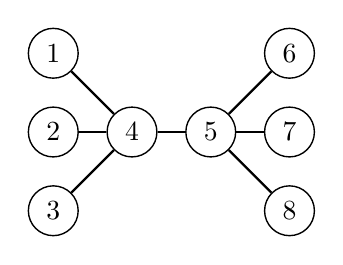
\begin{tikzpicture}
                \GraphInit
                \Vertex[x=-1, y=1, Lpos=180]{1}
                \Vertex[x=-1, y=0, Lpos=180]{2}
                \Vertex[x=-1, y=-1, Lpos=180]{3}
                \Vertex[x=0, y=0, Lpos=-90]{4}
                \Vertex[x=1, y=0, Lpos=-90]{5}
                \Vertex[x=2, y=1]{6}
                \Vertex[x=2, y=0]{7}
                \Vertex[x=2, y=-1]{8}
                \Edges(1,4,5,6)
                \Edges(2,4,3)
                \Edges(7,5,8)
            \end{tikzpicture}
        \end{center}

        The group $G = \Aut(\Gamma)$ of automorphisms of $\Gamma$ (relabellings of $\Gamma$ which preserve edges) acts naturally on $\Omega = V$, with the action of the automorphism $\sigma \in G$ on the vertex $v \in \Omega$ being $v^\sigma$. Then clearly $G \leq \Sym(8)$ is a permutation group of degree 8. Let $G^0 = \tilde G^0 = G = \Aut(\Gamma)$. We consider two stabiliser chains for $G$ (and find $|G|$):
        \begin{itemize}
            \item Let $G^1 = \added{2}{G^0_{4}}$. Then $4^{G^0} = \{4,5\}$, and take $T_1 = \{(),(1,6)(2,7)(3,8)(4,5)\}$. \\
                  Let $G^2 = \added{2}{G^1_{1}} = \added{2}{G_{4,1}}$. Then $1^{G^1} = \{1,2,3\}$, and take $T_1 = \{(),(1,2),(1,3)\}$. \\
                  Let $G^3 = \added{2}{G^2_{2}} = \added{2}{G_{4,1,2}}$. Then $2^{G^2} = \{2,3\}$, and take $T_2 = \{(),(2,3)\}$. \\
                  Let $G^4 = \added{2}{G^3_{6}} = \added{2}{G_{4,1,2,6}}$. Then $6^{G^3} = \{6,7,8\}$, and take $T_3 = \{(),(6,7),(6,8)\}$. \\
                  Let $G^5 = \added{2}{G^4_{7}} = \added{2}{G_{4,1,2,6,7}} = 1$. Then $7^{G^4} = \{7,8\}$, and take $T_4 = \{(),(7,8)\}$.

                  But $G^5 = 1$, since the only automorphism that fixes 4, 1, 2, 6, and 7 is the identity. So we see that $B = [4,1,2,6,7]$ is a nonredundant base for $G$ with stabiliser chain $G = G^0 > G^1 > G^2 > G^3 > G^4 > G^5 = 1$ and associated transversals $T_1,\dotsc,T_5$. A strong generating set $S$ for $G$ is $\{(1,6)(2,7)(3,8)(4,5),(1,2),(1,3),(2,3),(6,7),(6,8),(7,8)\}$, with size 7. Moreover, from \autoref{prop:stabiliser_chain_indexes}, we see that $|G| = |T_1| \dotsb |T_5| = 2 \cdot 3 \cdot 2 \cdot 3 \cdot 2 = 72$, so there are 72 automorphisms (relabellings) of $\Gamma$. % From \autoref{lem:transversal_gives_bsgs}, the size of a strong generating set $S$ for $G$ relative to $B$ is $\sum_i |T_i| - 5 = 7$.
            \item Let $\tilde G^1 = \added{2}{\tilde G^0_{1}}$. Then $|1^{\tilde G^0}| = 6 = |\tilde T_1|$, since an automorphism sends 1 to any leaf. \\
                  Let $\tilde G^2 = \added{2}{\tilde G^1_{2}} = \added{2}{G_{1,2}}$. Then $|2^{\tilde G^1}| = 2 = |\tilde T_2|$, since when 1 is fixed, so are 4 and 5. \\
                  Let $\tilde G^3 = \added{2}{\tilde G^2_{6}} = \added{2}{G_{1,2,6}}$. Then $|6^{\tilde G^2}| = 3 = |\tilde T_3|$, since when 1 and 2 are fixed, 6 can map to 6, 7 or 8. \\
                  Let $\tilde G^4 = \added{2}{\tilde G^3_{7}} = \added{2}{G_{1,2,6,7}}$. Then $|7^{\tilde G^3}| = 2 = |\tilde T_4|$, since (similar to above) the image of 7 is 7 or 8.

                  But $\tilde G^4 = 1$, since the only automorphism that fixes 1, 2, 6, and 7 is the identity. So we see that $\tilde B = [1,2,6,7]$ is a nonredundant base for $G$ with stabiliser chain $G = \tilde G^0 > \tilde G^1 > \tilde G^2 > \tilde G^3 > \tilde G^4 = 1$ and transversals $\tilde T_1,\dotsc,\tilde T_4$. As before, we see that $|G| = |\tilde T_1| \dotsb |\tilde T_4| = 6 \cdot 2 \cdot 3 \cdot 2 = 72$. % The size of a strong generating set $S'$ for $G$ relative to $\tilde B$ is $\sum_i |\tilde T_i| - 4 = 9$.
        \end{itemize}
        Note that any base $B$ for $G$ must contain at least two of $\{1,2,3\}$ and two of $\{6,7,8\}$, otherwise there is an automorphism $\sigma \neq 1_{\Sym(\Omega)}$ that fixes $B$ but swaps two elements of $\{1,2,3\}$ or $\{6,7,8\}$ that are not in $B$. So $\added{2}{b(G)} = 4$.

        Also, note that while $\hat B = [1,2,6,7,4]$ is also a base for $G$ as a permutation of the (nonredundant) base $B = [4,1,2,6,7]$, we see that $\hat B$ is \textit{not} nonredundant since $\hat G^4 = \added{2}{G_{1,2,6,7}} = 1 = \added{2}{G_{1,2,6,7,4}} = \hat G^5$ from the second example.
    \end{example}}

\subsection{Random elements and the constructive membership problem}

In the above proof of \autoref{lem:transversal_gives_bsgs}, we found a \textit{unique} decomposition of $g \in G$ as a product of transversal elements $t_rt_{r-1}\dotsb t_1$ with each $t_i \in T_i$. This gives us a simple way of generating random elements in $G$, \added{1}{or simply enumerating all elements of $G$,} assuming we have transversals of the stabiliser chain; these can be computed using the \hyperref[alg:orbit_stabiliser]{orbit-stabiliser algorithm}.

\begin{algorithm}[random element]\label{alg:transversal_random_element}
    Let $B = [\beta_1,\dotsc,\beta_r]$ be a base for $G \leq \Sym(\Omega)$ and $\mathcal{T} := [T_1,\dotsc,T_r]$ be the corresponding transversals of the stabiliser chain. \added{1}{For each transversal $T_i$, choose $t_i \in T_i$ \added{2}{independently and} uniformly at random, and return $g = t_rt_{r-1}\dotsb t_1 \in G$ which is a random element in $G$.}
\end{algorithm}

Note that this corresponds to a uniform distribution on $G$, since for fixed $\tilde g = \tilde t_r\tilde t_{r-1}\dotsb\tilde t_1 \in G$, \added{2}{independence and} uniqueness of the decomposition gives that the probability of randomly choosing $\tilde g$ is
$$\PR(g = \tilde g) = \PR(t_1 = \tilde t_1,\dotsc,t_r = \tilde t_r) = \PR(t_1 = \tilde t_1) \dotsb \PR(t_r = \tilde t_r) = \frac{1}{|T_1|} \dotsb \frac{1}{|T_r|} = \frac{1}{|G|}.$$
\added{4}{Moreover, we can clearly generate an independent and identically distributed (uniform) random sample $g_1,\dotsc,g_n$ from $G$ by repeating this procedure.} See the \hyperref[app:transversal_random_element]{appendix} for an implementation in \texttt{GAP} as the function \texttt{RandomElt}.

\added{4}{This is useful, since alternatives to getting a random element in a finitely generated large group $G = \langle x_1,\dotsc,x_m\rangle$ may be to use a random product of generators and inverses of random length (a na\"ive approach that has no reason a priori to have favourable statistical properties), or possibly a more sophisticated approach as found in \cite{celler1995}, which generates a list of random elements of $G$ at the expense of independence and uniformity (which is only asymptotically true).}

\begin{example}\label{eg:automorphism_group_graph_random}
    Recall from \autoref{eg:automorphism_group_graph_bsgs} the graph $\Gamma$ with vertex set $V = \{1,\dotsc,8\}$, the stabiliser chain $G = G^0 > G^1 > G^2 > G^3 > G^4 > G^5 = 1$ for $G = \Aut(\Gamma)$, and the strong generating set
    $$S = \{(1,6)(2,7)(3,8)(4,5),(1,2),(1,3),(2,3),(6,7),(6,8),(7,8)\}$$
    for $G$. Using \texttt{GAP}, we may define $G$ as the group generated by $S$:

    \lstinputlisting{txt_files/automorphism_group_graph_bsgs_gap.gap}

    The following \texttt{GAP} code assumes \texttt{G}, \texttt{B} and \texttt{SC} are defined as above. Let us run through \autoref{alg:transversal_random_element} to generate a random element of $G$. Below is \texttt{GAP} code with a modified \texttt{RandomElt} function that prints out the choices of $t_i \in T_i$ (and the intermediate calculations for constructing random $g \in G$; see appendix).

    \lstinputlisting{txt_files/automorphism_group_graph_bsgs_gap_2.gap}

    So here, the algorithm chooses $t_1 = (1,6)(2,7)(3,8)(4,5) \in T_1$, $t_2 = (1,2) \in T_2$, $t_3 = (2,3) \in T_3$, $t_4 = () \in T_4$, $t_5 = (7,8) \in T_5$, and returns $g = t_5 t_4 t_3 t_2 t_1 = (1,7,3,6)(2,8)(4,5) \in G$, \added{4}{a uniformly random automorphism of $\Gamma$.}
\end{example}

Next we consider a na\"ive algorithm to test membership of $g \in \Sym(\Omega)$ in a permutation group $G \leq \Sym(\Omega)$ given a BSGS for $G$ arising from transversals for the stabiliser chain:

\begin{algorithm}[membership test]\label{alg:transversal_membership_test}
    Let $B = [\beta_1,\dotsc,\beta_r]$ be a base for $G \leq \Sym(\Omega)$ and $\mathcal{T} := [T_1,\dotsc,T_r]$ be the corresponding transversals of the stabiliser chain. For arbitrary $g \in \Sym(\Omega)$, to test if $g \in G$, we do the following:

    \begin{algorithmic}[1]
        \Procedure{Membership}{$G,\Omega,B,\mathcal{T},g$}\Comment{Whether $g \in G$}
        \State $h \gets g$
        \For{$i \gets 1$ \textbf{to} $r$}\Comment{We go through each stabiliser $G^{i-1}$}
        \added{1}{\If{$\beta_i^h = \beta_i^{t_i}$ for some $t_i \in T_i$} $h \gets ht_i^{-1}$\Comment{$\beta_i^{ht_i^{-1}} = \beta_i$; here we set $h = gt_1^{-1} t_2^{-1} \dotsb t_i^{-1}$}
        \Else\ \Return \texttt{False}\label{alg:transversal_membership_test:not_in_orbit}
        \EndIf}
        \EndFor
        \added{1}{\If{$h = 1$} \Return \texttt{True}\label{alg:transversal_membership_test:1_ending}
            \Else\ \Return \texttt{False}\label{alg:transversal_membership_test:not_1_ending}
            \EndIf}
        \EndProcedure
    \end{algorithmic}
\end{algorithm}

\added{1}{\begin{proof}[Proof of correctness]
        This algorithm simultaneously deals with the cases that $g \in G$ and $g \not\in G$. First, consider the case that $g \in G$. For each $i$, we find $t_i \in T_i$ with $h = gt_1^{-1} t_2^{-1} \dotsb t_r^{-1} \in G^r = 1$ in line \ref{alg:transversal_membership_test:1_ending}, so $g = t_r t_{r - 1} \dotsb t_1 \in G$, and we return \texttt{True}.

        If $g \not\in G$, suppose for a contradiction that \added{3}{we return \texttt{True}. Then $h = 1$ with $h = gt_1^{-1}\dotsb t_r^{-1}$ and $t_1,\dotsc,t_r \in G$, so $g = t_r t_{r - 1} \dotsb t_1 \in G$, which is a contradiction.}
    \end{proof}}

See the \hyperref[app:transversal_membership_test]{appendix} for an implementation in \texttt{GAP} as the function \texttt{Membership}.

\added{1}{\begin{example}\label{eg:automorphism_group_graph_membership}
        Recall from \autoref{eg:automorphism_group_graph_bsgs} the graph $\Gamma$ with vertex set $V = \{1,\dotsc,8\}$, and the stabiliser chain $G = G^0 > G^1 > G^2 > G^3 > G^4 > G^5 = 1$ for $G = \Aut(\Gamma)$. The following \texttt{GAP} code assumes \texttt{G}, \texttt{B} and \texttt{SC} are defined as in \autoref{eg:automorphism_group_graph_bsgs}. Let us run through \autoref{alg:transversal_membership_test} to show that $(1,3,5,2)(7,8) \not\in G$. Below is \texttt{GAP} code with a modified \texttt{Membership} function that prints out the values of $h$ and $t_i$ throughout the algorithm.

        \lstinputlisting{txt_files/automorphism_group_graph_bsgs_gap_3.gap}

        Recall that the base for $G$ is $[4,1,2,6,7]$. Set $h = (1,3,5,2)(7,8)$ and suppose for contradiction that $h \in G$.
        \begin{itemize}
            \item For $i = 1$: $4^h = 4$ and we choose $t_1 = () \in T_1$. Then we redefine $h \gets ht_1^{-1} = (1,3,5,2)(7,8) \in G^1$.
            \item For $i = 2$: $1^h = 2$ and we choose $t_2 = (1,3) \in T_2$. Then we redefine $h \gets ht_2^{-1} = (2,3,5)(7,8) \in G^2$.
            \item For $i = 3$: $2^h = 3$ and we choose $t_3 = (2,3) \in T_3$. Then we redefine $h \gets ht_3^{-1} = (3,5)(7,8) \in G^3$.
            \item For $i = 4$: $6^h = 6$ and we choose $t_4 = () \in T_4$. Then we redefine $h \gets ht_4^{-1} = (3,5)(7,8) \in G^4$.
            \item For $i = 5$: $7^h = 8$ and we choose $t_5 = (7,8) \in T_5$. Then we redefine $h \gets ht_5^{-1} = (3,5)\in G^5 = 1$.
        \end{itemize}
        This is clearly a contradiction, as $(3,5) \neq ()$. So $h \not\in G$. (Note that if one of the base element images was not in the relevant orbit, we would stop the algorithm earlier and also conclude non-membership in $G$.)
    \end{example}}

\added{1}{We have not yet answered the question of how we \textit{find} a BSGS for a permutation group $G$. One such way is the \hyperref[alg:schreier_sims]{Schreier-Sims algorithm}. However, to discuss this, we first discuss an algorithm for computing orbits, stabilisers and transversals.}

\subsection{The orbit-stabiliser and Schreier-Sims algorithms}

\added{1}{To get the stabiliser chain for a base $B$, we must store information about the pointwise stabilisers of an elements in $B$. We can do this by finding a generating set for each stabiliser. Furthermore, it is useful to store transversals of the stabiliser chain for various purposes such as membership testing and random element generation; these \added{2}{can all be} found by the orbit-stabiliser algorithm.}

\begin{algorithm}[orbit-stabiliser]\label{alg:orbit_stabiliser}
    Suppose $G = \langle X \rangle$ is finitely generated by $X = [x_1,\dotsc,x_m]$ and acts on $\Omega$. Let $\alpha \in \Omega$. Suppose further that the orbit $\alpha^G$ is finite. The following algorithm computes $\alpha^G$, a generating set for $\added{2}{G_\alpha}$, and a right transversal $T$ of $\added{2}{G_\alpha}$:

    (Denote the $i$th element of the ordered list $L$ by $L[i]$, and the concatenation of lists $L_1,L_2$ by $L_1 \cup L_2$.)

    \begin{algorithmic}[1]
        \Procedure{OrbitStabiliser}{$G = \langle X \rangle,\Omega,\alpha$}\Comment{Computes the $G$-orbit and \added{2}{generating set of} stabiliser (and its transversal) of $\alpha$}
        \State $\mathcal{O} \gets [\alpha]$, $T \gets [1]$, $S \gets [\ ]$, $\mathcal{E} \gets X \cup X^{-1} = [x_1,\dotsc,x_m,x_1^{-1},\dotsc,x_m^{-1}]$, $i \gets 1$
        \While{$i \leq |\mathcal{O}|$}\label{alg:orbit_stabiliser:i_while_loop}
        \State $o \gets \mathcal{O}[i]$\Comment{$o = \mathcal{O}[i] = \alpha^{T[i]}$}
        \For{$x \in \mathcal{E}$}\label{alg:orbit_stabiliser:x_for_loop}
        \If{$o^x \not\in \mathcal{O}$} append $o^x$ to $\mathcal{O}$, $T[i]x$ to $T$\Comment{$\mathcal{O}[\ell + 1] := o^x = \alpha^{T[i]x} = \alpha^{T[\ell + 1]}$ where $\ell = |\mathcal{O}|$}\label{alg:orbit_stabiliser:append_to_O_T}
        \added{1}{\ElsIf{$o^x = \mathcal{O}[j]$ for some $j$}} append $T[i]xT[j]^{-1}$ to $S$\Comment{$\alpha^{T[i]x} = o^x = \alpha^{T[j]}$ so $\alpha^{T[i]xT[j]^{-1}} = \alpha$}\label{alg:orbit_stabiliser:already_in_O}
        \EndIf
        \EndFor
        \State $i \gets i + 1$
        \EndWhile
        \State \Return $\mathcal{O},T,S$\Comment{The orbit is $\mathcal{O}$, $S$ generates the stabiliser, $T$ is a transversal}
        \EndProcedure
    \end{algorithmic}

    Then $\mathcal{O} = \alpha^G$, $\langle S \rangle = \added{2}{G_\alpha}$, and $T$ is a transversal of $\added{2}{G_\alpha}$ in $G$.
\end{algorithm}

% TODO: Cite something for the stabiliser?

Next we show that the algorithm works (and terminates), but we omit the proof that $\langle S \rangle = \added{2}{G_\alpha}$ for brevity \added{3}{(see Section 4.1 of \cite{holt_handbook_cgt2005} for proof)}. The key to this algorithm is that $\mathcal{O}[i] = \alpha^{T[i]}$ for all $i$, from $\mathcal{O}[1] = \alpha = \alpha^1 = \alpha^{T[1]}$ and the comment in line \ref{alg:orbit_stabiliser:append_to_O_T}.

\begin{proof}
    Observe that $T \subseteq G$ since we only append elements of the form $T[i]x$ to $T$ whenever line \ref{alg:orbit_stabiliser:append_to_O_T} runs, where $T[i] \in T \subseteq G$ (since $T[1] = 1 \in G$ and then by induction on $i$) and $x \in \mathcal{E} \subseteq G$.

    First we show that $\mathcal{O} = \alpha^G$. Clearly $\mathcal{O} \subseteq \alpha^G$: if $o \in \mathcal{O}$ then $o = \mathcal{O}[i]$ for some $i$, so $o = \mathcal{O}[i] = \alpha^{T[i]}$ where $T[i] \in T \subseteq G$. To see that $\alpha^G \subseteq \mathcal{O}$: take $\alpha^g \in \alpha^G$ where $g \in G$. Then $g = x_{i_1}^{\varepsilon_1}\dotsb x_{i_k}^{\varepsilon_k}$ with each $\varepsilon_{i_j} = \pm 1$ since $G = \langle X \rangle$ is finitely generated. We proceed by induction on $k$. If $k = 0$, then $g = 1$ and $\alpha^g = \alpha^1 = \alpha = \mathcal{O}[1] \in \mathcal{O}$. For the inductive step with $k \geq 1$, write
    $$\alpha^g = \alpha^{x_{i_1}^{\varepsilon_1}\dotsb x_{i_k}^{\varepsilon_k}} = \left(\alpha^{x_{i_1}^{\varepsilon_1}\dotsb x_{i_{k - 1}}^{\varepsilon_{k - 1}}}\right)^{x_{i_k}^{\varepsilon_k}};$$
    by the inductive hypothesis $\alpha^{x_{i_1}^{\varepsilon_1}\dotsb x_{i_{k - 1}}^{\varepsilon_{k - 1}}} \in \mathcal{O}$, say $\alpha^{x_{i_1}^{\varepsilon_1}\dotsb x_{i_{k - 1}}^{\varepsilon_{k - 1}}} = \mathcal{O}[\ell]$ for some $\ell$. Then when $i = \ell$ (in line \ref{alg:orbit_stabiliser:i_while_loop}) and $x = x_{i_k}^{\varepsilon_k} \in \mathcal{E}$ (in line \ref{alg:orbit_stabiliser:x_for_loop}), we append $\alpha^g = o^{x_{i_k}^{\varepsilon_k}}$ to $\mathcal{O}$. So indeed $\mathcal{O} = \alpha^G$. Since $\alpha^G$ is finite, the algorithm terminates (see line \ref{alg:orbit_stabiliser:i_while_loop}).

    \added{1}{By line \ref{alg:orbit_stabiliser:append_to_O_T}, we see that at the end of the algorithm, $T$ comprises elements $t \in G$ with $\alpha^t$ all distinct and $\{\alpha^t\}_{t \in T} = \alpha^G$. Then \autoref{cor:orbit_stabiliser_transversal} implies $T$ is a transversal of $\added{2}{G_\alpha}$ in $G$.}
\end{proof}

Now a subgroup of a finitely generated group need not be finitely generated; it is known that the free group on 2 generators has a subgroup isomorphic to a free group on a countably infinitely set of generators. However, the \hyperref[alg:orbit_stabiliser]{orbit-stabiliser algorithm} proves that for any finitely generated group $G$ acting on a set $\Omega$, if an orbit $\alpha^G$ is finite, then the stabiliser $\added{2}{G_\alpha}$ is finitely generated:

\begin{corollary}\label{cor:stabiliser_is_finitely_generated}
    Let a finitely generated group $G = \langle X \rangle$ act on $\Omega$ and $\alpha \in G$. If $\alpha^G$ is finite, then $\added{2}{G_\alpha}$ is finitely generated (by the output $S$ of the \hyperref[alg:orbit_stabiliser]{orbit-stabiliser algorithm}, which is finite with $|S| \leq 2|\alpha^G||X|$). \qedhere
\end{corollary}

\added{1}{Now that we have established a way of computing orbits, stabilisers and transversals, we can look to a general form of computing a BSGS for a permutation group $G$. One such approach is the \textbf{Schreier-Sims algorithm}, if a partial base $B$ and generating set $S$ for $G$ are known.\label{alg:schreier_sims} \added{2}{(Often, we have the empty partial base $B = [\ ]$, which we ``extend'' to find a base for $G$.)}

% Intuitively, for each point $\beta_i$ in $B$, we calculate \textit{Schreier generators} for $G^i = \added{2}{G^{i-1}_{\beta_i}} = \added{2}{G_{\beta_1,\dotsc,\beta_i}}$; the union of these Schreier generators for the $G^i$ forms a strong generating set $S$ for $G$. To calculate Schreier generators for $G^i$, which are of the form $t_ix\tilde t_i^{-1}$ where $t_i,\tilde t_i \in T_i$ (a right transversal of $G^i$ in $G^{i-1}$) and $x \in X$ (where $G = \langle X \rangle$), we use the \hyperref[alg:orbit_stabiliser]{orbit-stabiliser algorithm} to compute the orbit $\beta_i^{G^{i-1}}$ and transversal $T_i$. However, some of the Schreier generators are the identity in $G$, so we can ignore them.
% we extend $B$ to a base for $G$ by che

Intuitively, a na\"ive version of the algorithm extends $B$ to a base by considering generators $x \not\in \added{2}{G_{\beta_1,\dotsc,\beta_k}}$ in $S$ and appending points of $\Omega$ that are not fixed by $x$. We then use the \hyperref[alg:orbit_stabiliser]{orbit-stabiliser algorithm} to compute and append \textit{Schreier generators} for $G^i = \added{2}{G_{\beta_1,\dotsc,\beta_i}}$ to $S$, ignoring those that are equal to the identity $1 \in G$. The resulting $(B,S)$ is a BSGS for $G$, and is an improvement over \autoref{lem:transversal_gives_bsgs}.

% TODO: GIVE INTUITON (extend $B$ to base, use OST to compute orbits/stabilisers/transversals for subsequent thingies in stab chain, but use Schreier generators to reduce the size of SGS). Below is an outline of the procedure:

% \begin{algorithm}[Schreier-Sims]\label{alg:schreier_sims}
%     Let $B = [\beta_1,\dotsc,\beta_k]$ be an initial sequence (possibly empty) of distinct elements of $\Omega$, and $G = \langle X \rangle \leq \Sym(\Omega)$ a permutation group. We extend $B$ to a base for $G$ and extend $X$ to a strong generating set $S$ for $G$:

%     \begin{algorithmic}[1]
%         \Procedure{SchreierSims}{$B,\Omega,X$}\Comment{Extends $B$ to a base for $G$, and extends $X$ to a strong generating set $S$}

%         TODO: COMPLETE
%         \State $S \gets X$
%         \For{$x \in S$}
%         \If{$x \in \added{2}{G_{\beta_1,\dotsc,\beta_k}}$} append $\gamma \in \Omega$ to $B$ where $\gamma^x \neq \gamma$
%         \State $k \gets k + 1$
%         \EndIf
%         \EndFor
%         \State $S_i = S \cap \added{2}{G_{\beta_1,\dotsc,\beta_i}}$
%         % \State $\mathcal{O} \gets [\alpha]$, $T \gets [1]$, $S \gets [\ ]$, $\mathcal{E} \gets X \cup X^{-1} = [x_1,\dotsc,x_n,x_1^{-1},\dotsc,x_n^{-1}]$, $i \gets 1$
%         % \While{$i \leq |\mathcal{O}|$}\label{alg:orbit_stabiliser:i_while_loop}
%         % \State $o \gets \mathcal{O}[i]$\Comment{$o = \mathcal{O}[i] = \alpha^{T[i]}$}
%         % \For{$x \in \mathcal{E}$}\label{alg:orbit_stabiliser:x_for_loop}
%         % \If{$o^x \not\in \mathcal{O}$} append $o^x$ to $\mathcal{O}$, $T[i]x$ to $T$\Comment{$\mathcal{O}[\ell + 1] := o^x = \alpha^{T[i]x} = \alpha^{T[\ell + 1]}$ where $\ell = |\mathcal{O}|$}\label{alg:orbit_stabiliser:append_to_O_T}
%         % \added{1}{\ElsIf{$o^x = \mathcal{O}[j]$ for some $j$}} append $T[i]xT[j]^{-1}$ to $S$\Comment{$\alpha^{T[i]x} = o^x = \alpha^{T[j]}$ so $\alpha^{T[i]xT[j]^{-1}} = \alpha$}\label{alg:orbit_stabiliser:already_in_O}
%         % \EndIf
%         % \EndFor
%         % \State $i \gets i + 1$
%         % \EndWhile
%         % \State \Return $\mathcal{O},T,S$\Comment{The orbit is $\mathcal{O}$, $S$ generates the stabiliser, $T$ is a transversal}
%         \EndProcedure
%     \end{algorithmic}

%     We return $(B,S)$ which is now a BSGS for $G$.
% \end{algorithm}

This algorithm was used by Sims to construct and prove existence of some of the theorised sporadic finite simple groups, such as Lyons' group (degree $n \approx 9 \cdot 10^6$) in 1973 \cite{sims1973}. It is implemented in many computational packages such as \texttt{GAP} to compute bases, and for large degree groups, a randomised variant is used to speed up computation since the number of Schreier generators to be processed becomes too large for the deterministic algorithm.}

\section{Overview of classification results}

The definitions and results in this section are primarily found in \cite{rotman_intro_theory_groups1995} and \cite{dixon_mortimer_perm_groups1996}.

\subsection{Elementary abelian groups}

In chapter 4, we will need the notion of an elementary abelian $p$-group, which we then realise as a permutation group.

\begin{definition}\label{def:p-group}
    Let $p$ be a prime. A \textbf{$p$-group} is a group $G$ in which every element has order a power of $p$. An \textbf{elementary abelian ($p$-)group} $G$ is an abelian group in which every nontrivial element has order $p$.
\end{definition}

It can be shown that $G$ is a finite $p$-group if and only if the order of $G$ is a power of $p$. One such proof uses Sylow's theorems, the first of which is presented below without proof. Recall that a \textbf{maximal subgroup} $H$ of $G$ is a subgroup $H \leq G$ such that $H < K \leq G$ implies $K = G$.

\begin{definition}\label{def:sylow_subgroup}
    Let $G$ be a group. A \textbf{Sylow $p$-subgroup} of $G$ is a maximal $p$-subgroup of $G$, i.e. a maximal subgroup with order a power of $p$.
\end{definition}

\begin{theorem}[Sylow (1)]\label{thm:sylow}
    Let $G$ be a finite group and $p$ a prime that divides $|G|$. If $p^k$ is the maximal power of $p$ that divides $|G|$, then there exists a Sylow $p$-subgroup of order $p^k$.
\end{theorem}

One may use the theory of group actions to prove Sylow's theorem; see Theorem 4.17 in \cite{rotman_intro_theory_groups1995} for Wielandt's proof in this direction.

\begin{corollary}\label{cor:p-group_iff_prime_power_order}
    A group $G$ is a finite $p$-group if and only if the order of $G$ is a power of $p$.
\end{corollary}

\begin{proof}
    The case that $G = 1$ is trivial. Thus suppose $G \neq 1$ is a finite $p$-group and $q$ is a prime divisor of $|G|$. Let $q^k$ be the maximal power of $q$ that divides $|G|$. By Sylow's first theorem (\autoref{thm:sylow}), there is a Sylow $q$-subgroup $H \leq G$ with order $q^k$. Since $H \neq 1$, there is $h \in H$ with $\langle h \rangle \leq H$, so the order of $h$ divides $|H| = q^k$ by Lagrange's theorem. So $h$ has order a power of $q$, but $h \in G$ and $G$ is a $p$-group, so $q = p$, i.e. $|G|$ is a power of $p$. The converse result follows directly from Lagrange's theorem.
\end{proof}

Recall that for groups $G,H$, their \textbf{direct product} is the group $G \times H$ with underlying set the Cartesian product $G \times H$ and group operation $(g,h)(a,b) = (ga,hb)$ for $g,a \in G$ and $h,b \in H$. When $G$ and $H$ are \textit{abelian}, we may instead call it a \textbf{direct sum} and write $G \oplus H$; we often use additive notation $(g,h) + (a,b) = (g+a,h+b)$ with identity $0$, writing $ng$ instead of $g^n$.

It turns out that the structure of a finite abelian group is quite simple. The following result is standard; see Theorem 6.9 in \cite{rotman_intro_theory_groups1995} for a proof.

\begin{theorem}[Basis for finite abelian groups]\label{thm:basis_finite_abelian}
    Every finite abelian group $G$ is a direct sum of cyclic groups.
\end{theorem}

Using this result, we may show that a finite elementary $p$-group must be a direct sum of copies of $\Z/p\Z$.

\begin{corollary}\label{cor:elementary_abelian_group_form}
    If $G$ is a finite elementary abelian $p$-group, then $G \cong (\Z/p\Z)^k$ for some $k$. (In the literature, such $G \cong (\Z/p\Z)^k$ is often denoted by $p^k$.)
\end{corollary}

\begin{proof}
    By the basis theorem (\autoref{thm:basis_finite_abelian}), write $G \cong (\Z/n_1\Z) \oplus \dotsb \oplus (\Z/n_k\Z)$ with each $n_i > 1$. Let $e_i$ be the element in $(\Z/n_1\Z) \oplus \dotsb \oplus (\Z/n_k\Z)$ with a 1 in the $i$th entry and 0s elsewhere. Using the isomorphism, $e_i$ has order $p$ (since $G$ is elementary abelian), so $p1 = 0$ in $\Z/n_i\Z$, so $n_i = p$ (as $p$ is prime). Since $1 \leq i \leq k$ was arbitrary, the result follows.
\end{proof}

\subsection{Classification of finite simple groups}

Prime numbers are the ``building blocks'' of natural numbers, in the sense that a natural number has a unique factorisation as a product of prime numbers, by the fundamental theorem of arithmetic. Thus, to study number theory, it is often useful to study primes. A similar question arises for groups, in particular finite groups -- is there a way to break down an arbitrary finite group into the simplest ``building blocks''? The analogous object to prime numbers for groups is the notion of a simple group, which all finite groups can be decomposed into. (The inverse problem of reconstructing groups from simple groups is more difficult than for integers, and is referred to as the group extension problem.)

The classification of finite simple groups is one of the most famous problems in group theory, and its statement and proof was achieved by a collaboration of many group theorists across many decades and many volumes of work. In \cite{solomon2001}, Solomon notes that computational group theory has also been influential in the classification result: for instance, by 2001, computer algorithms were being created to identify permutation groups, linear groups and ``black box'' groups, and calculations of groups of order $2^{10}$ re-verified the fact that ``most'' finite groups are nilpotent groups of nilpotence class at most 2.

Recall that a \textbf{maximal normal subgroup} of a nontrivial group $G$ is a normal subgroup $1 \neq N \lhd G$ such that $N \lhd M \unlhd G$ implies $M = G$.

\begin{definition}\label{def:simple_group}
    A group $G \neq 1$ is \textbf{simple} if it has no nontrivial normal subgroups.
\end{definition}

\added{3}{For example, the cyclic groups $C_p$ of prime order are simple by Lagrange's theorem; if $n = uv$ is not prime, then $C_n = \langle a \rangle$ is not simple since $1 \neq \langle a^u \rangle \lhd C_n$. Moreover, $\Alt(n)$ is simple for $n \geq 5$.} Now, by the correspondence theorem (see Theorem 2.28 in \cite{rotman_intro_theory_groups1995}), $N \unlhd G$ is a maximal normal subgroup of $G$ if and only if $G/N$ is simple. \added{3}{This is because a normal subgroup of $G/N$ is of the form $M/N$ with $N \unlhd M \unlhd G$, and $M = N$ (in which case $M/N \cong 1$) or $M = G$ (which implies simplicity of $G/N$) if and only if $N$ is maximal in $G$.}

\begin{definition}\label{def:group_extension}
    Let $N,Q$ be groups. A group $G$ is an \textbf{extension} of $N$ by $Q$ if there is a normal subgroup $N \cong N^* \unlhd G$ with $G/N^* \cong Q$; we write $G = N \mathrel{.} Q$. \added{3}{(This is equivalent to saying that $G$ factors over $N$ with quotient $Q$.)}
\end{definition}

Here, we think of $Q$ as the quotient after we factor out the ``normal subgroup'' $N$ of $G$. For example, the direct product $G \times H$ is an extension of $G$ by $H$ and an extension of $H$ by $G$; the subgroups $G \times 1$ and $1 \times H$ are normal in $G \times H$. \added{3}{Note that there may be nonisomorphic groups $G$ that satisfy $G = N \mathrel{.} Q$ for given groups $N,Q$. For example, set $N = Q = C_2$. The groups $G = C_4 = \langle a \rangle$ and $\tilde G = C_2 \times C_2$ (where $C_2 = \langle b \rangle$) are nonisomorphic, yet $G/\langle a^2 \rangle \cong Q$ and $\tilde G/\langle (b,1) \rangle \cong Q$ with $\langle a^2 \rangle \cong N \cong \langle (b,1) \rangle$. Thus, there is, in general, no unique way to reconstruct groups from their factors, and this is part of the difficulty of the group extension problem.}

\added{3}{This notation $G = N \mathrel{.} Q$ is ATLAS notation, and is often used in finite group theory. Note that often a cyclic group $C_n$ is simply written as $n$ (e.g. $2 \mathrel{.} \Alt(5) = \Sym(5)$), an elementary abelian $p$-group $(\Z/p\Z)^d$ as $p^d$, and an unspecified group of order $n$ as $[n]$.}

\added{3}{\begin{definition}\label{def:composition_series}
    A \textbf{composition series} is a finite subgroup series $G = N_0 \rhd N_1 \rhd \dotsb \rhd N_r = 1$ where each $N_{i+1}$ is a \textit{maximal} normal subgroup of $N_i$. The quotient groups $N_i/N_{i+1}$ are the \textbf{composition factors}.

    We say that two composition series $G = N_0 \rhd N_1 \rhd \dotsb \rhd N_r = 1$ and $G = \tilde N_0 \rhd \tilde N_1 \rhd \dotsb \rhd \tilde N_{\tilde r} = 1$ of a group $G$ are \textbf{equivalent} if there is a bijection between the composition factors such that corresponding composition factors are isomorphic.
\end{definition}

Clearly, if $G = N_0 \rhd N_1 \rhd \dotsb \rhd N_r = 1$ is a composition series, then the composition factors $N_i/N_{i+1}$ are simple, since the $N_{i+1}$ are maximal in $N_i$. Moreover, if $G$ is finite, then a composition series exists, since maximal subgroups exist (and the groups in the series decrease in size).

\begin{example}\label{eg:composition_series}
    Consider the cyclic group $C_{12} = \langle a \rangle$. Two composition series are $C_{12} \rhd \langle a^2 \rangle \rhd \langle a^4 \rangle \rhd 1$ and $C_{12} \rhd \langle a^2 \rangle \rhd \langle a^6 \rangle \rhd 1$. The composition factors of the first series are $C_{12}/\langle a^2 \rangle \cong C_2$, $\langle a^2 \rangle/\langle a^4 \rangle \cong C_2$ and $\langle a^4 \rangle/1 \cong C_3$, while the composition factors of the second series are $C_{12}/\langle a^2 \rangle \cong C_2$, $\langle a^2 \rangle/\langle a^6 \rangle \cong C_3$ and $\langle a^6 \rangle/1 \cong C_2$. Both composition series have the same length, 3, and the composition factors can be paired up, so the two series are equivalent.
\end{example}

The amazing fact is that for every group (possibly infinite) that has a composition series, every composition series is equivalent! This is the Jordan-H\"older theorem, which is proven as Theorem 5.12 in \cite{rotman_intro_theory_groups1995}:

\begin{theorem}[Jordan-H\"older]\label{thm:jordan_holder}
    Any two composition series of a group $G$ are equivalent.
\end{theorem}

A fun corollary of this result is the fundamental theorem of arithmetic:

\begin{corollary}[Fundamental theorem of arithmetic]\label{cor:fundamental_thm_arithmetic}
    An integer $n \geq 2$ has a unique factorisation as a product of primes.
\end{corollary}

\begin{proof}
    We apply \autoref{thm:jordan_holder} to the group $C_n = \langle a \rangle$. First note that $C_n$ has a composition series $C_n = N_0 \rhd N_1 \rhd \dotsb \rhd N_r = 1$ with each $N_i/N_{i+1}$ simple. Since all subgroups of $C_n$ are cyclic, we have that each $N_i = \langle a^{n_i} \rangle$, and $N_i/N_{i+1} = \langle a^{n_i} \rangle/\langle a^{n_{i+1}} \rangle \cong C_{n_{i+1}/n_i}$ is simple, thus $n_{i+1}/n_i = p_{i+1}$ for some prime $p_{i+1}$. But then $1 = \langle a^n \rangle$ and $n_0 = 1$, so
    $$n = n_r = (n_1/n_0)(n_2/n_1) \dotsb (n_r/n_{r-1}) = p_1 p_2 \dotsb p_r,$$
    so $n$ has a factorisation into primes.

    Now, any product of primes $p_i$ that equals $n$ gives rise to a composition series: if $n = p_1 \dotsb p_r$, then $G = \langle a \rangle \rhd \langle a^{p_1} \rangle \rhd \langle a^{p_1 p_2} \rangle \rhd \dotsb \rhd \langle a^{p_1 \dotsb p_r} \rangle = 1$ is a composition series (since the quotient groups have prime order $p_i$, thus simple). Then by Jordan-H\"older, any two composition series are equivalent, so the composition factors of the two series are isomorphic after permutation, and it follows that the primes in the resulting factorisations are the same up to rearrangement.
\end{proof}

Another consequence of the Jordan-H\"older theorem is that if $G$ is a group with composition series $G = N_0 \rhd N_1 \rhd \dotsb \rhd N_r = 1$ and composition factors $N_{i-1}/N_i = Q_i$, then $N_{i-1} = N_i \mathrel{.} Q_i$ and thus
$$G = N_0 = N_1 \mathrel{.} Q_1 = \dotsb = ((\dotsb(N_r \mathrel{.} Q_r)\mathrel{.}\dotsb )\mathrel{.} Q_2)\mathrel{.} Q_1 = ((\dotsb(Q_r \mathrel{.} Q_{r-1})\mathrel{.} \dotsb)\mathrel{.} Q_2)\mathrel{.} Q_1 = Q_r \mathrel{.} \dotsb \mathrel{.} Q_1,$$
with the composition factors $Q_i$ determined uniquely by $G$. Thus if we knew all finite simple groups, and we could solve the extension problem, then we could classify all finite groups.

Now, the extension problem asks one to ``determine'' all groups $G$ such that $G/N \cong Q$ for given $N,Q$. One such approach is that we may construct a multiplication table for any such $G$; \cite{rotman_intro_theory_groups1995} notes that Schreier solved the problem in this sense. However, if we require that the isomorphism classes of $G$ can be characterised, \cite{rotman_intro_theory_groups1995} notes that no solution is known. On the other hand, the classification of finite simple groups is complete, and the following may be found in \cite{solomon2018}:

\begin{theorem}[Classification of finite simple groups]\label{thm:cfsg}
    Every finite simple group is isomorphic to one of the following:
    \begin{enumerate}[(a)]
        \item a cyclic group $C_p$ of prime order $p$,
        \item an alternating group $\Alt(n)$ of degree $n \geq 5$,
        \item a simple group of \textbf{Lie type}, or
        \item one of 26 \textbf{sporadic simple groups}.
    \end{enumerate}
\end{theorem}}

\subsection{Semidirect products and wreath products}

Recall again that for groups $G,N$, their \textbf{direct product} is the group $G \times N$ with underlying set the Cartesian product $G \times N$ and group operation $(g,n)(h,m) = (gh,nm)$ for $g,h \in G$ and $n,m \in H$. Now, in some scenarios, the underlying set of a group is naturally the Cartesian product $G \times N$, but the group operation is not the direct product. For example, the underlying set of the dihedral group $D_{2n} = \{1,r,\dotsc,r^{n-1},s,sr,\dotsc,sr^{n-1}\}$ is naturally $C_2 \times C_n = \{1,s\} \times \{1,r,\dotsc,r^{n-1}\}$ via the map $(s^a,r^b) \mapsto s^ar^b \in D_{2n}$. If $G$ acts on $N$ while respecting the group structure on $N$, we can define a more general type of product on the set $G \times N$, called the \textit{semidirect product}, that turns it into a group.

\begin{definition}\label{def:semidirect_product}
    Let $G,N$ be groups and suppose $G$ acts on $N$ via a homomorphism $\varphi : G \to \Aut(N)$. The \textbf{semidirect product} of $G$ and $N$ (with respect to $\varphi$), denoted $G \ltimes_\varphi N$ (or simply $G \ltimes N$ if clear from context), is a group with underlying set the Cartesian product $G \times N$ and group operation $(g,n)(h,m) = (gh,n^hm)$ for $g,h \in G$ and $n,m \in N$.
\end{definition}

We omit the proof that $G \ltimes N$ is a group, but observe that $|G \ltimes N| = |G||N|$, and for $g \in G$ and $n,m \in N$, we have $(nm)^g = n^g m^g$ and $(n^{-1})^g = (n^g)^{-1}$ since $\varphi(g) \in \Aut(N)$. Moreover, the identity in $G \ltimes N$ is $(1,1)$, and inverses are given by $(g,n)^{-1} = (g^{-1},(n^{-1})^{g^{-1}}) = (g^{-1},(n^{g^{-1}})^{-1})$. Note that some sources (such as \cite{dixon_mortimer_perm_groups1996}) alternatively define the semidirect product as $N \rtimes G$ (with underlying set $N \times G$) with group operation $(n,g)(m,h) = (nm^{g^{-1}},gh)$.

The semidirect product $G \ltimes N$ has \added{3}{a subgroup $G^* = \{(g,1) : g \in G\} \cong G$ and} a normal subgroup $N^* = \{(1,n) : n \in N\} \cong N$, since $(g,m)^{-1}(1,n)(g,m) = (g^{-1},(m^{-1})^{g^{-1}})(g,n^gm) = (1,m^{-1}n^gm) \in N^*$ for $g \in G$ and $n,m \in N$. Note that when $\varphi$ is the trivial map (i.e. $g \mapsto 1_{\Aut(N)}$ for all $g \in G$), we recover the direct product, since $n^h = n$ for all $n \in N$ and $h \in G$.

\begin{example}\label{eg:D8_semidirect_product}
    The dihedral group $D_8 = \{1,r,r^2,r^3,s,sr,sr^2,sr^3\}$ of symmetries of a square can be realised as a semidirect product $C_2 \ltimes C_4$, where $C_2 = \{1,s\}$ acts on $C_4 = \{1,r,r^2,r^3\}$ by $1 \mapsto ()$ and $s \mapsto (r,r^3)$ (inversion). The isomorphism $C_2 \ltimes C_4 \to D_8$ is then simply $(g,h) \mapsto gh \in D_8$ (for $g \in C_2$ and $h \in C_4$). An interpretation of this is: to compose two symmetries $s^ar^b$ and $s^ur^v$ in $D_8$, the reflection components compose directly (to yield $s^{a+u}$), but the rotation component may be affected (yielding the direct composition $(r^b)^{s^u} r^v = r^{b+v}$ if $s^u = 1$, or $r^{-b+v}$ otherwise).

    We can verify that this is consistent with our permutation representation $r \sim (1,2,3,4)$ and $s \sim (1,4)(2,3)$ for $D_8$ in \autoref{eg:action_D8_on_square}. Note that in $C_2 \ltimes C_4$, $(s,1)(1,r) = (s1,1^1r) = (s,r)$ and $(1,r)(s,1) = (1s,r^s1) = (s,r^3)$. In the permutation representation, $sr = (2,4)$ and $(r,s) = (1,3) = sr^3$, which is compatible with the isomorphism $C_2 \ltimes C_4 \to D_8$ above.

    This generalises to the dihedral group $D_{2n}$, which is isomorphic to the semidirect product $C_2 \ltimes C_n$ where $C_2 = \{1,s\}$ acts on $C_n = \{1,r,\dotsc,r^{n-1}\}$ by $1 \mapsto ()$ and $s \mapsto (r^a \mapsto r^{-a})$ (inversion). The isomorphism $C_2 \ltimes C_n \to D_{2n}$ is $(g,h) \mapsto gh \in D_{2n}$; \added{3}{$D_{2n}$ thus has a normal subgroup isomorphic to $C_n$ (which is the group of rotations).}
\end{example}

Semidirect products are related to the notion of a split extension.

\begin{definition}\label{def:split_extension}
    If $G$ is a group and $Q,N$ are subgroups with $N \unlhd G$, $G = QN$ and $Q \cap N = 1$, then $G$ is a \textbf{split extension} of $N$ by $Q$, and write $G = N : Q$. \added{3}{We say that $G$ \textbf{splits} over $N$.} (Recall that $QN = \{qn : q \in Q,n \in N\}$.)
\end{definition}

\begin{lemma}\label{lem:split_extensions_are_semidirect_products}
    If $G = N : Q$ for $N,Q \leq G$, then $G \cong Q \ltimes_\varphi N$ where $\varphi : Q \to \Aut(N)$ is the conjugation action given by $n^g = g^{-1}ng$ for $n \in N$ and $g \in Q$.
\end{lemma}

Note that the order of the factors are reversed in $N : Q$ compared to $Q \ltimes N$. This follows from the fact that the semidirect product is alternatively defined as $N \rtimes Q$, as seen earlier. We now prove the above lemma:

\begin{proof}
    Consider the map $\psi : Q \ltimes_\varphi N \to N : Q$ with $(g,n) \mapsto gn$. Note that an element of $N : Q = QN$ can be uniquely expressed as $gn$ with $g \in Q$ and $n \in N$: suppose $gn = hm$ for $g,h \in Q$ and $n,m \in N$. Then $Q \ni h^{-1}g = mn^{-1} \in N$, so $h = g$ and $m = n$ since $Q \cap N = 1$. Thus $\psi$ is clearly a bijection.

    Now for $(g,n),(h,m) \in Q \ltimes_\varphi N$,
    $$\psi((g,n)(h,m)) = \psi((gh,n^hm)) = ghn^hm = gh(h^{-1}nh)m = (gn)(hm) = \psi((g,n))\psi((h,m)),$$
    so $\psi$ is a homomorphism, thus an isomorphism.
\end{proof}

The proof of this lemma also allows us to see that the \textit{split extension} $N : Q$ is indeed an \textit{extension} of $N$ by $Q$ (see \autoref{def:group_extension}), since $N \unlhd G$ with $G/N \cong Q$ via the homomorphism $\varphi : G \to Q$ where $qn \mapsto q$. Well-definition follows from the unique decomposition of elements in $G = N : Q = QN$ in the proof above; indeed $\varphi((gn)(hm)) = \varphi(gh(h^{-1}nh)m) = gh = \varphi(gn)\varphi(hm)$ for $gn,hm \in QN$ since $h^{-1}nh \in N \unlhd G$; finally $\varphi$ is clearly surjective and its kernel is clearly $N$, so the result follows from the first isomorphism theorem.

\added{3}{Now, \autoref{eg:D8_semidirect_product} shows that the semidirect product construction $G \ltimes_\varphi N$ may lead to nonisomorphic groups with different choice of $\varphi$, so as with general extensions, split extensions are not unique. Suppose $D_8 \cong C_2 \ltimes_\varphi C_4$, so that $D_8 = C_4 \mathrel{.} C_2$. However, the direct product $C_2 \times C_4$ is also a split extension (semidirect product) that is not isomorphic to $D_8$ (one is abelian, the other is not).}

A special type of semidirect product, called the wreath product, plays an important role in the study of primitive \added{3}{and imprimitive} permutation groups.

\added{3}{\begin{definition}\label{def:function_group}
    Let $G$ be a group and $X$ a set. Then $G^X$ is the \textbf{group of functions $X \to G$}, which is a group under pointwise multiplication: for $\omega,\eta \in G^X$ and $x \in X$, $\omega\eta(x) = \omega(x)\eta(x) \in G$.
\end{definition}

The proof that $G^X$ forms a group is straightforward; the identity is $1$, defined by $x \mapsto 1 \in G$; the inverse is defined pointwise. Note that in this context, $G^X$ does not denote the image of $G$ under an action on $X$.

\begin{definition}\label{def:wreath_product}
    Given groups $G$ and $H$ and suppose $G$ acts on $\Omega \neq \emptyset$. Then the \textbf{wreath product} $H \wr_\Omega G$ of $H$ by $G$ is the semidirect product $G \ltimes H^\Omega$ where $G$ acts on $H^\Omega$, with $\omega^g \in H^\Omega$ given by $\alpha \mapsto \omega(\alpha^{g^{-1}})$ for $\omega \in H^\Omega$ and $g \in G$.

    The \textbf{base group} of the wreath product $H \wr_\Omega G = G \ltimes H^\Omega$ is the subgroup $\{(1,\omega) : \omega \in H^\Omega\} \cong H^\Omega$.
\end{definition}

Note that for $\omega \in H^\Omega$, $\alpha \in \Omega$ and $g,h \in G$, $\omega^{gh}(\alpha) = \omega(\alpha^{h^{-1}g^{-1}}) = \omega^g(\alpha^{h^{-1}}) = (\omega^g)^h(\alpha)$, so $\omega^{gh} = (\omega^g)^h$. Moreover, $\omega^1(\alpha) = \omega(\alpha^1) = \omega(\alpha)$, so $\omega^1 = \omega$; together, these imply that this is indeed a $G$-action. If $\varphi$ is the $G$-action on $H^\Omega$ in this definition, then indeed $\varphi : G \to \Aut(H^\Omega)$, so that we have a semidirect product: for $\omega,\eta \in H^\Omega$, $\alpha \in \Omega$ and $g \in G$,
$$\omega^g\eta^g(\alpha) = \omega^g(\alpha)\eta^g(\alpha) = \omega(\alpha^{g^{-1}})\eta(\alpha^{g^{-1}}) = \omega\eta(\alpha^{g^{-1}}) = (\omega\eta)^g(\alpha),$$
so $(\omega\eta)^g = \omega^g\eta^g$, as required. Note that $|H \wr_\Omega G| = |H|^{|\Omega|} |G|$.

In the case that $\Omega = [n]$, we may identify the base group of the wreath product $H \wr_\Omega G$ with the direct product $H^n$ (via the isomorphism $H^{\Omega} \to H^n$ where $(\omega : \Omega \to H) \mapsto (\omega(1),\dotsc,\omega(n))$), so that $H \wr_\Omega G = G \ltimes H^n$. The action of $G$ on $H^n$ corresponds to permuting components: $g \in G$ acts on $(\omega_1,\dotsc,\omega_n) \in H^n$ by permuting components according to $g$, with $(\omega_1,\dotsc,\omega_n)^g = (\omega_{1_g},\dotsc,\omega_{n_g})$ where $i_g = i^{g^{-1}}$. Then an element of $H \wr_\Omega G$ is $(g,\omega_1,\dotsc,\omega_n)$ with $g \in G$ and each $\omega_i \in H$, and the product in $H \wr_\Omega G$ is given by
$$(g,\omega_1,\dotsc,\omega_n)(h,\eta_1,\dotsc,\eta_n) = (gh,\omega_{1_h}\eta_1,\dotsc,\omega_{n_h}\eta_n)$$
where each $i_h = i^{h^{-1}}$. If we further have $G = \Sym(n)$ which acts naturally on $[n]$, then we write $H \wr \Sym(n)$ instead of $H \wr_\Omega \Sym(n)$.

We discuss two important actions of the wreath product. The imprimitive action is natural and relates to imprimitive groups, while the product action is important in the classification of finite primitive groups.

\begin{definition}\label{def:imprimitive_action}
    Suppose $G$ acts on $\Omega$ and $H$ acts on $\Gamma$. Let $W = H \wr_\Omega G$; the \textbf{imprimitive action} of $W$ on $\Omega \times \Gamma$ is given by the following: for $(g,\omega) \in W = G \ltimes H^\Omega$ and $(\alpha,\gamma) \in \Omega \times \Gamma$ we define
    $$(\alpha,\gamma)^{(g,\omega)} = (\alpha^g,\gamma^{\omega(\alpha^g)}).$$
\end{definition}

This is indeed an action: for $(\alpha,\gamma) \in \Omega \times \Gamma$ and $(g,\omega),(h,\eta) \in W$,
$$((\alpha,\gamma)^{(g,\omega)})^{(h,\eta)} = (\alpha^g,\gamma^{\omega(\alpha^g)})^{(h,\eta)} = (\alpha^{gh},\gamma^{\omega(\alpha^g)\eta(\alpha^{gh})}) = (\alpha^{gh},\gamma^{\omega^h\eta(\alpha^{gh})}) = (\alpha,\gamma)^{(gh,\omega^h\eta)} = (\alpha,\gamma)^{(g,\omega)(h,\eta)}$$
since $\omega^h\eta(\alpha^{gh}) = \omega^h(\alpha^{gh})\eta(\alpha^{gh}) = \omega(\alpha^g)\eta(\alpha^{gh})$. Also, $(\alpha,\gamma)^{(1,1)} = (\alpha^1,\gamma^{1(\alpha^1)}) = (\alpha,\gamma^{1_H}) = (\alpha,\gamma)$.

In the case that $\Omega = [n]$, using the identification $H^\Omega \to H^n$ from above, the imprimitive action corresponds to $(i,\gamma)^{(g,\omega_1,\dotsc,\omega_n)} = (i^g,\gamma^{\omega_{i^g}})$ for $(i,\gamma) \in \Omega \times \Gamma$, $g \in G$ and $(\omega_1,\dotsc,\omega_n) \in H^n$.

\begin{proposition}
    Suppose $G$ acts on $\Omega$ via $\varphi_G$ and $H$ acts on $\Gamma$ via $\varphi_H$. Let $\hat\varphi$ be the imprimitive action of $W = H \wr_\Omega G$ on $\Omega \times \Gamma$. Then $\Ker\hat\varphi = \Ker\varphi_G \times \{\omega \in H^\Omega : \omega[\Omega] \subseteq \Ker\varphi_H\}$. Thus, the imprimitive action $\hat\varphi$ of $W = H \wr_\Omega G$ on $\Omega \times \Gamma$ is faithful if and only if the $G$-action $\varphi$ and $H$-action $\tilde\varphi$ are both faithful.
\end{proposition}

\begin{proof}
    Note that
    \begin{align*}
        \Ker\hat\varphi & = \{(g,\omega) \in W : (\alpha^g,\gamma^{\omega(\alpha^g)}) = (\alpha,\gamma)^{(g,\omega)} = (\alpha,\gamma)\ \text{for all}\ (\alpha,\gamma) \in \Omega \times \Gamma\}      \\
                        & = \{(g,\omega) \in W : g \in G_\alpha\ \text{for all}\ \alpha \in \Omega\ \text{and}\ \omega(\alpha) \in H_\gamma\ \text{for all}\ (\alpha,\gamma) \in \Omega \times \Gamma\} \\
                        & = \{(g,\omega) \in W : g \in \Ker\varphi_G\ \text{and}\ \omega(\alpha) \in \Ker\varphi_H\ \text{for all}\ \alpha \in \Omega\}                                                 \\
                        & = \Ker\varphi_G \times \{\omega \in H^\Omega : \omega[\Omega] \subseteq \Ker\varphi_H\}.
    \end{align*}
    Then if $\varphi_G,\varphi_H$ are faithful (i.e. $\Ker\varphi_G = 1_G$ and $\Ker\varphi_H = 1_H$), then $\omega[\Omega] \subseteq 1_H$ if and only if $\omega = 1 \in H^\Omega$, so $\Ker\hat\varphi = 1_G \times 1_{H^\Omega} = 1_W$, and the imprimitive action is faithful. Conversely, if the imprimitive action is faithful, then $\Ker\varphi_G = 1_G$ and $\{\omega \in H^\Omega : \omega[\Omega] \subseteq \Ker\varphi_H\} = 1_{H^\Omega}$, so $\Ker\varphi_H = 1_H$ (consider a constant map in $H^\Omega$) and the result follows.
\end{proof}

Now, the image $W^{\Omega \times \Gamma}$ of the imprimitive action is a subgroup of $\Sym(\Omega \times \Gamma)$. So, if $G \leq \Sym(\Omega)$ and $H \leq \Sym(\Gamma)$ have the natural action (which is faithful), then $W$ embeds as a subgroup of $\Sym(\Omega \times \Gamma)$.

\begin{lemma}\label{lem:imprimitive_action_is_imprimitive}
    Suppose $G$ acts transitively on $\Omega$ and $H$ acts primitively on $\Gamma$, with $|\Omega|,|\Gamma| > 1$. Then the imprimitive action of $W = H \wr_\Omega G$ on $\Omega \times \Gamma$ is imprimitive with $\Sigma = \{\{\alpha\} \times \Gamma : \alpha \in \Omega\}$ a system of imprimitivity.
\end{lemma}

\begin{proof}
    The action is transitive: for $(\alpha,\gamma),(\tilde\alpha,\tilde\gamma) \in \Omega \times \Delta$, we have $\tilde\alpha = \alpha^g$ for some $g \in G$, and $\tilde\gamma = \gamma^h$ for some $h \in H$. Then let $\omega \in H^\Omega$ be the constant map $\beta \mapsto h$; then $(\alpha,\gamma)^{(g,\omega)} = (\alpha^g,\gamma^{\omega(\alpha^g)}) = (\tilde\alpha,\gamma^h) = (\tilde\alpha,\tilde\gamma)$.

    Now each $\Delta = \{\alpha\} \times \Gamma$ is a block for $\alpha \in \Omega$ with $|\Delta| = |\Gamma|$; it is nontrivial as long as $|\Omega|,|\Gamma| > 1$ so that $|\Delta| > 1$ and $\Delta \neq \Omega \times \Gamma$. We verify that it is a block: for any $(g,\omega) \in W$,
    $$\Delta^{(g,\omega)} = \{(\alpha,\gamma)^{(g,\omega)} : \gamma \in \Gamma\} = \{(\alpha^g,\gamma^{\omega(\alpha^g)}) : \gamma \in \Gamma\} = \{\alpha^g\} \times \Gamma^{\omega(\alpha^g)}$$
    with $\Gamma^{\omega(\alpha^g)} = \Gamma$ or $\Gamma^{\omega(\alpha^g)} \cap \Gamma = \emptyset$ by primitivity of $H^\Gamma$. In the first case, and assuming $\alpha^g = \alpha$, then $\Delta^{(g,\omega)} = \{\alpha\} \times \Gamma = \Delta$; otherwise, $\Gamma^{\omega(\alpha^g)} \cap \Gamma = \emptyset$ or $\alpha^g \neq \alpha$, in which case $\Delta^{(g,\omega)} \cap \Delta = \emptyset$. So $W^{\Omega \times \Gamma}$ is imprimitive as long as $|\Omega|,|\Gamma| > 1$.
\end{proof}}

\added{3}{If $G \leq \Sym(n)$ and $H \leq \Sym(m)$, consider the wreath product $W = H \wr_{[n]} G = G \ltimes H^n$. Note that $H$ acts on the ordered list $[1,\dotsc,m]$; let the $i$th copy of $H$ act on $X_i = [(i-1)m+1,\dotsc,im]$ (in the natural way). Let $X = \bigcup_{1 \leq i \leq n} X_i = [1,\dotsc,mn]$. Since $G$ acts on $\{1,\dotsc,n\}$, we now let $G$ act on $\{X_1,\dotsc,X_n\}$ by permutation. This allows us to consider $W$ as a subgroup of $\Sym(X) = \Sym(mn)$ instead of $\Sym([n] \times [m])$ (using the map $[n] \times [m] \to [mn]$ where $(i,j) \mapsto (i-1)m + j$). In particular, the $X_i$ form blocks and we have a block system $\Sigma = [X_1,\dotsc,X_n]$; the imprimitive action of $(g,\omega_1,\dotsc,\omega_n) \in W$ corresponds to permuting within each block $X_i$ by $\omega_i \in H \leq \Sym(m)$, then permuting the blocks in $\Sigma$ by $g \in G \leq \Sym(n)$.}

\added{3}{\begin{example}\label{eg:S2_wr_S2_isom_D8}
        Let $G = H = \Sym(2)$ and consider the wreath product $W = H \wr G = \Sym(2) \wr \Sym(2)$. Since $H = \Sym(2)$ is primitive (\autoref{eg:natural_action_Sn_blocks}) and $G = \Sym(2)$ is transitive, \autoref{lem:imprimitive_action_is_imprimitive} shows that $W$ acts imprimitively on $\Omega = \{1,2\} \times \{1,2\}$ with nontrivial block system $\Sigma = \{\{1\} \times \{1,2\},\{2\} \times \{1,2\}\}$.

        Now relabel $\Omega$ using $\tau : \Omega \to [4]$, where $(1,1) \mapsto 1$, $(1,2) \mapsto 3$, $(2,1) \mapsto 2$, and $(2,2) \mapsto 4$. Then $W$ acts imprimitively on $[4]$ in the following way: for $(g,\omega_1,\omega_2) \in W$ for $g,\omega_1,\omega_2 \in \Sym(2)$, if $\tau((m,n)) = i$ for $m,n \in [2]$, then we set
        $$i^{(g,\omega_1,\omega_2)} = \tau((m,n)^{(g,\omega_1,\omega_2)}) = \tau((m^g,n^{\omega_{m^g}})).$$
        For example, $1^{((1,2),(1,2),())} = \tau((1,1)^{((1,2),(1,2),())}) = \tau((1^{(1,2)},1^{()})) = \tau((2,1)) = 2$ but $1^{((1,2),(),(1,2))} = \tau((1^{(1,2)},1^{(1,2)})) = \tau((2,2)) = 4$. Since both actions are faithful, the imprimitive action is faithful and embeds into $\Sym(4)$. Calculation shows the following (see appendix for \texttt{GAP} code):
        \[\begin{array}{c|c|c|c|c|c|c}
                w \in W             & 1^w & 2^w & 3^w & 4^w & \psi(w) \in \Sym(4) & \tilde\psi(w) \in D_8 \\\hline
                ((),(),())          & 1   & 2   & 3   & 4   & ()                  & 1                     \\
                ((),(),(1,2))       & 1   & 4   & 3   & 2   & (2,4)               & sr                    \\
                ((),(1,2),())       & 3   & 2   & 1   & 4   & (1,3)               & sr^3                  \\
                ((),(1,2),(1,2))    & 3   & 4   & 1   & 2   & (1,3)(2,4)          & r^2                   \\
                ((1,2),(),())       & 2   & 1   & 4   & 3   & (1,2)(3,4)          & sr^2                  \\
                ((1,2),(),(1,2))    & 4   & 1   & 2   & 3   & (1,4,3,2)           & r^3                   \\
                ((1,2),(1,2),())    & 2   & 3   & 4   & 1   & (1,2,3,4)           & r                     \\
                ((1,2),(1,2),(1,2)) & 4   & 3   & 2   & 1   & (1,4)(2,3)          & s
            \end{array}\]
        The column with $\psi$ denotes an embedding $\psi : W \to \Sym(4)$, and the column with $\tilde\psi$ denotes an isomorphism $\tilde\psi : W \to D_8$, the dihedral group comprising symmetries of a square (see \autoref{eg:action_D8_on_square}; recall the embedding $D_8 = \langle r,s \rangle \to \Sym(4)$ via $r \mapsto (1,2,3,4)$ and $s \mapsto (1,4)(2,3)$).

        The corresponding system of imprimitivity is $\Sigma = [[1,3],[2,4]]$ (where we impose an ordering); for $w = (g,\omega_1,\omega_2) \in W$, we permute the first block $[1,3]$ according to $\omega_1$ and the second block $[2,4]$ according to $\omega_2$, then permute the blocks according to $g$, and consider the resulting permutation. (For example, $((1,2),(1,2),()) \in W$ corresponds to starting with $\Sigma = [[1,3],[2,4]]$, then permuting $[1,3]$ according to $\omega_1 = (1,2)$ and $[2,4]$ according to $\omega_2 = ()$ to get $[3,1]$ and $[2,4]$ respectively, then permuting blocks according to $g = (1,2)$ to get $[[2,4],[3,1]]$; the resulting permutation is $(1,2,3,4)$.)

        Using generators, we have that $W = \langle(1,2)\rangle \ltimes (\langle(1,2)\rangle \times \langle(1,2)\rangle)$. Note that $\langle(1,2)\rangle \times \langle(1,2)\rangle \cong \langle(1,3),(2,4)\rangle \leq \Sym(4)$; the group $\langle(1,2)\rangle$ acts on $\langle(1,2)\rangle \times \langle(1,2)\rangle$ by permuting components, so if we apply the relabelling $\tau$ we may see that $\langle(1,2)\rangle \ltimes (\langle(1,2)\rangle \times \langle(1,2)\rangle)$ is permutation isomorphic to $\langle(1,2)(3,4)\rangle \ltimes \langle(1,3),(2,4)\rangle$ where $\langle(1,2)(3,4)\rangle$ acts naturally on $\langle(1,3),(2,4)\rangle$. (Note that $(1,2)(3,4)$ acts naturally on the elements in $\Sigma = [[1,3],[2,4]]$ in the same way that $(1,2)$ permutes the blocks themselves.) So (omitting some details) we get an isomorphism
        \begin{multline*}
            \Sym(2) \wr \Sym(2) = \langle(1,2)\rangle \ltimes (\langle(1,2)\rangle \times \langle(1,2)\rangle) \cong \langle(1,2)(3,4)\rangle \ltimes \langle(1,3),(2,4)\rangle \\
            \cong \langle(1,2)(3,4),(1,3),(2,4)\rangle \cong \langle sr^2,sr,sr^3 \rangle = D_8.
        \end{multline*}
    \end{example}}

\added{3}{\begin{definition}\label{def:product_action}
    Suppose $G$ acts on $\Omega$ and $H$ acts on $\Gamma$. Let $W = H \wr_\Omega G$; the \textbf{product action} of $W$ on $\Gamma^\Omega = \{\phi \mid \phi : \Omega \to \Gamma\}$ is given by the following: for $(g,\omega) \in W = G \ltimes H^\Omega$ and $\phi \in \Gamma^\Omega$ we define $\phi^{(g,\omega)} \in \Gamma^\Omega$ by
    $$\alpha \mapsto \phi(\alpha^{g^{-1}})^{\omega(\alpha)}.$$
\end{definition}

The product action is indeed a $W$-action. First note that for $\phi \in \Gamma^\Omega$ and $\alpha \in \Omega$, $\phi^{(1,1)}(\alpha) = \phi(\alpha^1)^{1(\alpha)} = \phi(\alpha)$, so $\phi^{(1,1)} = \phi$. Then for $(g,\omega),(h,\eta) \in W$ and $\alpha \in \Omega$,
$$(\phi^{(g,\omega)})^{(h,\eta)}(\alpha) = \phi^{(g,\omega)}(\alpha^{h^{-1}})^{\eta(\alpha)} = \phi(\alpha^{h^{-1}g^{-1}})^{\omega(\alpha^{h^{-1}})\eta(\alpha)} = \phi(\alpha^{h^{-1}g^{-1}})^{\omega^h\eta(\alpha)} = \phi^{(gh,\omega^h\eta)}(\alpha),$$
so $(\phi^{(g,\omega)})^{(h,\eta)} = \phi^{(gh,\omega^h\eta)}$. The degree of the product action of $W$ is $|\Gamma|^{|\Omega|}$.

In the case that $\Omega = [n]$, we may identify $\Gamma^\Omega$ with $\Gamma^n$ via $(\phi : \Omega \to \Gamma) \mapsto (\phi(1),\dotsc,\phi(n)) \in \Gamma^n$. Then the product action corresponds to $(\phi_1,\dotsc,\phi_n)^{(g,\omega_1,\dotsc,\omega_n)} = (\phi_{1_g}^{\omega_1},\dotsc,\phi_{n_g}^{\omega_n})$ for $(\phi_1,\dotsc,\phi_n) \in \Gamma^n$, $g \in G$ and $(\omega_1,\dotsc,\omega_n) \in H^n$, where each $i_g = i^{g^{-1}}$. Thus, we permute the components of $(\phi_1,\dotsc,\phi_n)$ according to $g$, then apply the permutations $\omega_i$ to each component.}

\added{3}{\begin{example}\label{eg:product_action_Sm_subsets}
        Let $k \leq m$ and define an action of $\Sym(m)$ on $\binom{[m]}{k}$, the $k$-element subsets of $[m]$, by the following: for $\sigma \in \Sym(m)$ and $\{i_1,\dotsc,i_k\} \subseteq [m]$, let
        $$\{i_1,\dotsc,i_k\}^\sigma = \{i_1^\sigma,\dotsc,i_k^\sigma\}.$$
        This is an action: for $\{i_1,\dotsc,i_k\} \subseteq [m]$ and $\sigma,\tau \in \Sym(m)$, $\{i_1,\dotsc,i_k\}^1 = \{i_1^1,\dotsc,i_k^1\} = \{i_1,\dotsc,i_k\}$ and
        $$\{i_1,\dotsc,i_k\}^{\sigma\tau} = \{i_1^{\sigma\tau},\dotsc,i_k^{\sigma\tau}\} = \{i_1^\sigma,\dotsc,i_k^\sigma\}^\tau = (\{i_1,\dotsc,i_k\}^\sigma)^\tau.$$
        The degree of the action is $\binom{m}{k}$.

        Now consider the wreath product $\Sym(m) \wr \Sym(r)$ with the product action, where the action of $H = \Sym(m)$ is the above action on $k$-element subsets $\Gamma = \binom{[m]}{k}$ of $[m]$, and the action of $G = \Sym(r)$ is the natural action on $\Omega = [r]$. Here, the product action of the wreath product has degree $|\binom{[m]}{k}|^{|[r]|} = \binom{m}{k}^r$.

        For example, if $m = 3$, $r = 4$ and $k = 2$, with $g = (1,2,4) \in G$ and $(\omega_1,\omega_2,\omega_3,\omega_4) = ((),(1,2),(1,2,3),(2,3)) \in H^4$, we have (using the identification for $\Omega = [r]$) that
        \begin{multline*}
            (\underbrace{\{1,2\}}_{\phi_1},\underbrace{\{2,3\}}_{\phi_2},\underbrace{\{1,2\}}_{\phi_3},\underbrace{\{1,3\}}_{\phi_4})^{((1,2,4),(),(1,2),(1,2,3),(2,3))} = ({\underbrace{\{1,3\}}_{\phi_4}}^{()},{\underbrace{\{1,2\}}_{\phi_1}}^{(1,2)},{\underbrace{\{1,2\}}_{\phi_3}}^{(1,2,3)},{\underbrace{\{2,3\}}_{\phi_2}}^{(2,3)}) \\
            = (\{1^{()},3^{()}\},\{1^{(1,2)},2^{(1,2)}\},\{1^{(1,3,2)},2^{(1,3,2)}\},\{2^{(2,3)},3^{(2,3)}\}) = (\{1,3\},\{2,1\},\{3,1\},\{3,2\}) \in \Gamma^4.
        \end{multline*}
    \end{example}

    % TODO: PRODUCT ACTION FAITHFUL IFF ACTIONS OF EACH GROUP FAITHFUL?

    The following result gives a simple criterion for the product action of a wreath group to be primitive; see Lemma 2.7A in \cite{dixon_mortimer_perm_groups1996} for a proof.

    \begin{proposition}
        If nontrivial groups $G$ and $H$ act on $\Omega$ and $\Gamma$, then the wreath product $W = H \wr_\Omega G$ is primitive in the product action on $\Gamma^\Omega$ if and only if
        \begin{enumerate}[(i)]
            \item $H$ acts primitively but not regularly on $\Gamma$, and
            \item $\Omega$ is finite and $G$ acts transitively on $\Omega$.
        \end{enumerate}
    \end{proposition}}

\subsection{Matrix groups and affine groups}

The notion of an affine group is important for the later discussion and results in this \thesis{}. The following results may be found primarily in \cite{dixon_mortimer_perm_groups1996}.

\begin{definition}\label{def:gl_group}
    Let $K$ be a field and $V$ be a vector space over $K$. Let $\GL(V)$ be the \textbf{general linear group} over $V$, comprising invertible linear maps $V \to V$; note that $\GL(V) \leq \Sym(V)$, so $\GL(V)$ acts naturally on $V$. When $V$ is finite dimensional, $V \cong K^d$ for some integer $d$, and thus it suffices to consider the general linear group $\GL(K^d)$.

    Invertible linear maps $K^d \to K^d$ (or equivalently $V \to V$ given a choice of basis) may be represented by invertible $d \times d$ matrices in $M_d(K)$, which form the \textbf{general linear group $\GL_d(K)$ over $K$ of degree $d$} which is isomorphic to $\GL(K^d)$ (and thus $\GL(V)$). Alternatively, $\GL_d(K) = \{a \in M_d(K) : \det(a) \neq 0\}$. Note that $\GL_d(K)$ acts on $K^d$ by matrix multiplication: for $a \in \GL_d(K)$ and $u \in K^d$ a row vector, we have $u^a = ua$.

    When $K = \F_q$ is a finite field, we often write $\GL_d(q) = \GL_d(\F_q)$.
\end{definition}

The following definition comes from representation theory; see \autoref{eg:representations} for the definition of a representation.

\begin{definition}\label{def:irred_subgroup}
    Let $G \leq \GL_d(K)$ for some field $K$. A \textbf{$G$-invariant subspace} of $K^d$ is a subspace $W \leq K^d$ such that $wa \in W$ for all $w \in W$ and $a \in G$. Note that $0$ and $K^d$ are always $G$-invariant; these are the \textit{trivial invariant subspaces}.

    The subgroup $G \leq \GL_d(K)$ is \textbf{irreducible} if there are no nontrivial $G$-invariant subspaces (of $K^d$). (In other words, the \textit{setwise stabilisers} $G_W = \{a \in G : w^a = wa \in W\ \text{for all}\ w \in W\} \neq G$ for $0 < W < K^d$.)
\end{definition}

In the language of representation theory, we take $V = K^d$ in the above definition so that $\GL(V) \cong \GL_d(K)$, and the representation $\rho : G \to \GL(V)$ is simply the inclusion map; we identify $\rho$ with $G$, and irreducibility of $G$ corresponds with irreducibility of $\rho$.

\begin{definition}\label{def:affine_transformation}
    Let $K$ be a field and $d \geq 1$. For an invertible matrix $a \in \GL_d(K)$ and a row vector $v \in K^d$, the corresponding \textbf{affine transformation} $t_{a,v} : K^d \to K^d$ is given by $u \mapsto ua + v$ (where we think of $u \in K^d$ as a row vector).
\end{definition}

\begin{definition}\label{def:agl}
    The set of invertible affine transformations of $K^d$ forms a group under composition, called the \textbf{affine general linear group} of dimension $d \geq 1$ over $K$, and denoted by $\AGL_d(K) = \{t_{a,v} : a \in \GL_d(K), v \in K^d\}$.

    When $K = \F_q$ is a finite field, we often write $\AGL_d(q) = \AGL_d(\F_q)$. (Note that for a $d$-dimensional vector space $V$ over $K$, we may similarly define $\AGL(V) = \{t_{a,v} : a \in \GL(V), v \in V\}$ where $t_{a,v} : K \to K$ is given by $u \mapsto u^a + v$.)
\end{definition}

The following lemma proves that $\AGL_d(K)$ is indeed a group. In particular, it is a \added{3}{2-transitive} subgroup of $\Sym(K^d)$, the group of \textit{all} bijections $K^d \to K^d$. This shows $\AGL_d(K)$ is a \added{3}{primitive} permutation group that acts naturally on $K^d$ (\autoref{prop:2-transitivity_implies_primitivity}); if $K = \F_q$ is finite, $\AGL_d(q)$ has degree $q^d$. The group $\AGL_d(K)$ is of interest as it respects the affine structure on $K^d$.

\begin{lemma}\label{lem:agl_is_subgroup}
    Let $K$ be a field. The group $\AGL_d(K)$ is a 2-transitive subgroup of $\Sym(K^d)$. In particular, it has identity $1_{\AGL_d(K)} = t_{1,0}$, product $t_{a,v}t_{b,w} = t_{ab,vb+w}$, and inverses $t_{a,v}^{-1} = t_{a^{-1},-va^{-1}}$, for $t_{a,v},t_{b,w} \in \AGL_d(K)$.
\end{lemma}

\begin{proof}
    First, we show that $\AGL_d(K) \leq \Sym(K^d)$. Indeed, each $t_{a,v} \in \AGL_d(K)$ is a bijection with inverse $t_{a,v}^{-1} = t_{a^{-1},-va^{-1}}$ with $a^{-1} \in \GL_d(K)$ and $-va^{-1} \in K^d$: for $u \in K^d$,
    $$(u^{t_{a,v}})^{t_{a^{\scaleto{-1}{3pt}},-va^{\scaleto{-1}{3pt}}}} = (ua + v)^{t_{a^{\scaleto{-1}{3pt}},-va^{\scaleto{-1}{3pt}}}} = (ua + v)a^{-1} - va^{-1} = u$$
    and similarly $(u^{t_{a^{\scaleto{-1}{3pt}},-va^{\scaleto{-1}{3pt}}}})^{t_{a,v}} = u$. So $\AGL_d(K) \subseteq \Sym(K^d)$ (and is clearly non-empty, since the identity matrix $1 \in \GL_d(K)$ and $0 \in K^d$). This also shows $\AGL_d(K)$ is closed under inversion, since $t_{a,v}^{-1} = t_{a^{-1},-va^{-1}} \in \AGL_d(K)$.

    Now suppose $a,b \in \GL_d(K)$ and $v,w \in K^d$; then the composition
    $$t_{a,v}t_{b,w} = t_{ab,vb+w} \in \AGL_d(K)$$
    since $ab \in \GL_d(K)$, $vb + w \in K^d$, and for $u \in K^d$,
    $$(u^{t_{a,v}})^{t_{b,w}} = (ua + v)b + w = uab + (vb + w) = u^{t_{ab,vb+w}}.$$
    So indeed $\AGL_d(K) \leq \Sym(K^d)$; in particular, $\AGL_d(K)$ is a group under composition.

    Next we show $\AGL_d(K)$ is 2-transitive. Here, $\Sym(K^d)$ acts naturally on $\Omega = K^d$; since $\AGL_d(K) \leq \Sym(K^d)$, we take the natural action on $K^d$. Clearly $|\Omega| \geq 2$ (since $K$ is a field and $d \geq 1$). Suppose $[\alpha_1,\alpha_2]$ and $[\beta_1,\beta_2]$ are lists of distinct points in $K^d$; then extend $a_1 = \alpha_1 - \alpha_2 \neq 0$ and $b_1 = \beta_1 - \beta_2 \neq 0$ to bases $\{a_1,\dotsc,a_d\}$ and $\{b_1,\dotsc,b_d\}$ of $K^d$. Let $b,c$ be matrices (in $\GL_d(K)$ by construction) with rows $a_1,\dotsc,a_d$ and $b_1,\dotsc,b_d$ respectively.

    Let $c = a^{-1}b \in \GL_d(K) \iff b = ac \iff b_i = a_ic$ for all $1 \leq i \leq d$. Then $\beta_1 - \beta_2 = b_1 = a_1c = (\alpha_1 - \alpha_2)c \iff \beta_1 - \alpha_1 c = \beta_2 - \alpha_2 c$. Let $v = \beta_1 - \alpha_1c = \beta_2 - \alpha_2c \in K^d$, so that $[\beta_1,\beta_2] = [\alpha_1c + v,\alpha_2c + v] = [\alpha_1^{t_{c,v}},\alpha_2^{t_{c,v}}]$ with $t_{c,v} \in \AGL_d(K)$. So $\AGL_d(K)$ is 2-transitive.
\end{proof}

From this lemma, we see that affine groups arise as semidirect products of general linear groups over the underlying vector space. In particular, $|\AGL_d(K)| = |\GL_d(K)||K|^d$; if $K = \F_q$ is a finite field (with $|\F_q| = q$ a prime power), it can be shown that $|\AGL_d(q)| = q^d(q^d - 1)(q^d - q)\dotsb(q^d - q^{d-1})$ (here, the degree of the permutation group $\AGL_d(q)$ is $q^d$). The case that $q = 2$ is of particular interest, due to a question in \cite{moscatiello_roney-dougal2021} which we investigate.

\begin{proposition}\label{prop:agl_is_semidirect_product}
    The group $\AGL_d(K)$ is isomorphic to the semidirect product $\GL_d(K) \ltimes_\varphi K^d$ via the action $\varphi$ determined by $v^a = va \in K^d$ for $v \in K^d$ (viewed as a row vector) and $a \in \GL_d(K)$. (So $\AGL_d(K)$ has a subgroup isomorphic to $\GL_d(K)$ and a normal subgroup isomorphic to $K^d$.)
\end{proposition}

\begin{proof}
    This follows directly from the isomorphism $t_{a,v} \mapsto (a,v) \in \GL_d(K) \ltimes_\varphi K^d$, since $t_{a,v} t_{b,w} = t_{ab,vb+w}$ in $\AGL_d(K)$ (from \autoref{lem:agl_is_subgroup}) while $(a,v)(b,w) = (ab,v^b+w) = (ab,vb + w)$ in $\GL_d(K) \ltimes_\varphi K^d$ (by \autoref{def:semidirect_product}).
\end{proof}

\begin{proposition}\label{prop:agl_as_subgrp_of_gl}
    \begin{enumerate}[(a)]
        \item The group $\AGL_d(K) \leq \Sym(K^d)$ is permutation isomorphic to the subgroup
              $$G^* = \left\{
                  \begin{pmatrix}
                      a & 0   \\
                      v & 1_K
                  \end{pmatrix} : a \in \GL_d(K),v \in K^d\right\} \leq \GL_{d+1}(K) \leq \Sym(\Delta),$$
              where $\Delta = K^d \times \added{3}{\{1\}} \subseteq K^{d+1}$ is a block under the right-multiplication action \added{3}{of $G^*$} on $K^{d+1}$, and
        \item $b(\AGL_d(K)) = d + 1$, except that $b(\AGL_1(2)) = 1$ (where $d = 1$ and $K = \F_2$).
    \end{enumerate}
\end{proposition}

\begin{proof}
    \begin{enumerate}[(a)]
        \item The isomorphism $\psi : \AGL_d(K) \to G^*$ is given by
              $$t_{a,v} \mapsto \begin{pmatrix}
                      a & 0 \\
                      v & 1
                  \end{pmatrix};$$
              it is clearly bijective, and indeed $G^* \subseteq \GL_{d+1}(K)$: the rows $a_i \in K^d$ of $a \in \GL_d(K)$ form a basis for $K^d$, so the $\begin{pmatrix}
                      a_i & 0
                  \end{pmatrix} \in K^{d+1}$ (viewed as a row vector) are linearly independent for $i = 1,\dotsc,d$. In particular, adding $\begin{pmatrix}
                      v & 1
                  \end{pmatrix} \in K^{d+1}$ to this collection clearly preserves linear independence, and thus forms a basis for $K^{d+1}$.

              Recall from \autoref{lem:agl_is_subgroup} that, \added{3}{for $t_{a,v},t_{b,w} \in \AGL_d(K)$, }
              $$t_{a,v}t_{b,w} = t_{ab,vb+w}$$
              in $\AGL_d(K)$. \added{3}{This translates to}
              $$\begin{pmatrix}
                      a & 0 \\
                      v & 1
                  \end{pmatrix}
                  \begin{pmatrix}
                      b & 0 \\
                      w & 1
                  \end{pmatrix} =
                  \begin{pmatrix}
                      ab     & 0 \\
                      vb + w & 1
                  \end{pmatrix},$$
              in $G^*$. \added{3}{Thus} $\psi$ is a homomorphism (and the image $G^*$ is a subgroup of $\GL_{d+1}(K)$).

              Note that $G^* \leq \GL_{d+1}(K)$ acts on $K^{d+1}$ by matrix right-multiplication. In particular, $\Delta$ is a block under this action: for $\begin{pmatrix}
                      u & 1
                  \end{pmatrix} \in \Delta$ (viewed as a row vector, with $u \in K^d$), $a \in \GL_d(K)$ and $v \in K^d$, we have $ua + v \in K^d$, so
              $$\begin{pmatrix}
                      u & 1
                  \end{pmatrix}^{\left(
                  \begin{smallmatrix}
                          a & 0 \\
                          v & 1
                      \end{smallmatrix}\right)} =
                  \begin{pmatrix}
                      u & 1
                  \end{pmatrix}
                  \begin{pmatrix}
                      a & 0 \\
                      v & 1
                  \end{pmatrix} =
                  \begin{pmatrix}
                      ua + v & 1
                  \end{pmatrix} \in \Delta.$$
              Then $G^* = G^*_\Delta$, and \autoref{lem:restrict_action_to_block}(b) implies $G^*$ acts on $\Delta$.

              Define $\tau : K^d \to \Delta$ by $u \mapsto
                  \begin{pmatrix}
                      u & 1
                  \end{pmatrix} \in K^{d+1}$ (clearly a bijection). Then for $u \in K^d$ and $t_{a,v} \in \AGL_d(K)$, we have
              $$\tau(u^{t_{a,v}}) = \tau(ua + v) =
                  \begin{pmatrix}
                      ua + v & 1
                  \end{pmatrix} =
                  \begin{pmatrix}
                      u & 1
                  \end{pmatrix}
                  \begin{pmatrix}
                      a & 0 \\
                      v & 1
                  \end{pmatrix} = \tau(u)
                  \begin{pmatrix}
                      a & 0 \\
                      v & 1
                  \end{pmatrix} = \tau(u)^{\left(
                      \begin{smallmatrix}
                          a & 0 \\
                          v & 1
                      \end{smallmatrix}\right)} = \tau(u)^{\psi(t_{a,v})},$$
              so $\AGL_d(K)$ and $G^*$ are permutation isomorphic via $\tau$ and $\psi$.
        \item Note that $B = [e_1,\dotsc,e_{d+1}]$ is a base for $G^*$, where the $(e_i)$ are the standard basis for $K^{d+1}$. This follows from the fact that for $a \in \GL_d(K)$ and $v \in K^d$,
              $$e_i^{\left(
                  \begin{smallmatrix}
                          a & 0 \\
                          v & 1
                      \end{smallmatrix}\right)} = e_i
                  \begin{pmatrix}
                      a & 0 \\
                      v & 1
                  \end{pmatrix} = e_i$$
              for all $i$ if and only if the $i$th row of the matrix is $e_i$ for all $i$, so the matrix is the identity (and $a = 1,v = 0$). (In fact, any basis for $K^{d+1}$ forms a base for $G^*$.) So $b(\AGL_d(K)) = b(G^*) \leq d + 1$ (using \autoref{lem:perm_isom_base}(c)). If $d = 1$ and $K = \F_2$, note that $[0]$ is a base for $\AGL_1(2)$, since if $0^{t_{a,v}} = 0$ then $v = 0a + v = 0$ and $a = 1$ (since $K^* = 1$).

              Now suppose $B = [u_1,\dotsc,u_d] \subseteq K^d$ are all distinct. Then for $k \leq d$ and with $G = \AGL_d(K)$, we have $G_{u_1,\dotsc,u_d} \leq G_{u_1,\dotsc,u_k}$, so if $G_{u_1,\dotsc,u_d} \neq 1$, then $[u_1,\dotsc,u_k]$ is certainly not a base for $G$. Now we claim that $B$ is not a base for $G$. If $d = 1$ and $K \neq \F_2$, then if $u_1 = 0$, then there is $1 \neq a \in K^*$ such that $0^{t_{a,0}} = 0a + 0 = 0$, so $B$ is not a base for $G$. If $u_1 \neq 0$, then set $u_1 \neq v \in K^*$ (such $v$ exists) and $a = u_1^{-1}(u_1 - v) \in K^*$, then $u_1^{t_{a,v}} = u_1a + v = u_1u_1^{-1}(u_1 - v) + v = u_1$, and $B$ is not a base for $G$.

              Now suppose $d \geq 2$. If $\{u_1,\dotsc,u_d\}$ are linearly independent (and form a basis for $K^d$), let $b \in \GL_d(K)$ be the matrix with rows $u_i$, and let $c$ be the matrix with rows $u_i - v$, where $v = u_1 - u_2 \neq 0$. Since $\Span_K\{u_1 - v,u_2 - v\} = \Span_K\{u_2,2u_2 - u_1\} = \Span_K\{u_1,u_2\}$, it follows that
              $$\Span_K\{u_1 - v,u_2 - v,\dotsc,u_d - v\} = \Span_K\{u_1,u_2,u_3 - v,\dotsc,u_d - v\} = \Span_K\{u_1,u_2,\dotsc,u_d\} = K^d,$$
              so $\{u_1 - v,u_2 - v,\dotsc,u_d - v\}$ is linearly independent, and thus $c \in \GL_d(K)$. Now set $a = b^{-1}c \in \GL_d(K)$ (recall $v = u_1 - u_2 \neq 0$); then $t_{a,v} \neq \Id_{K^d}$ satisfies
              $$u_i^{t_{a,v}} = u_ia + v = u_ib^{-1}c + v = e_ic + v = (u_i - v) + v = u_i$$
              for $i = 1,\dotsc,d$ (where $e_i$ is the $i$th standard basis vector in $K^d$), and $B$ is not a base for $G$.

              If $\{u_1,\dotsc,u_d\}$ are linearly dependent, let $U = \Span_K\{u_1,\dotsc,u_d\}$ and write $K^d = U \oplus W$ for some nontrivial subspace $W \leq K^d$. Set $v = 0$ and take $a \in \GL(K^d)$ such that $a|_U = \Id_U$ and $a|_W \neq \Id_W$. Then $u_i^{t_{a,v}} = u_ia + v = u_i$ for $i = 1,\dotsc,d$, so that $t_{a,v} \in G_{(B)}$, but $w^{t_{a,v}} = wa + v = wa \neq w$ for some $w \in W$, so $t_{a,v} \neq \Id_{K^d}$. Thus $B$ is not a base for $G$.

              From these two cases, we get that $b(\AGL_d(K)) > d$. So $b(\AGL_d(K)) = d + 1$, as claimed.
    \end{enumerate}
\end{proof}

\added{3}{Finally, we look at a few important subgroups of the affine group, which we consider again later. This next result expands upon \autoref{prop:agl_is_semidirect_product}.

    \begin{proposition}\label{prop:subgroups_of_agl}
        \begin{enumerate}[(a)]
            \item The general linear group $\GL_d(K) \cong \GL(K^d) = \{t_{a,0} : a \in \GL_d(K)\} \leq \AGL_d(K)$ acts transitively on the nonzero vectors $K^d \setminus 0$.
            \item The \textbf{translation subgroup} $T = \{t_{1,v} : v \in K^d\} \unlhd \AGL_d(K)$ is a minimal normal subgroup of $\AGL_d(K)$. Moreover, $T \cong K^d$ and $\AGL_d(K)/T \cong \GL_d(K)$. % (Recall that for $v \in K^d$, $t_{1,v} : K^d \to K^d$ is given by $u \mapsto u + v$.)
            \item The group $\AGL_d(K)$ splits over the translation subgroup $T$, and $\AGL_d(K) = \GL(K^d)T$.
        \end{enumerate}
    \end{proposition}

    \begin{proof}
        \begin{enumerate}[(a)]
            \item Clearly $\GL(K^d)$ is a subgroup of $\AGL_d(K)$ by the subgroup criterion, since $t_{a,0}t_{b,0} = t_{ab,0}$ and $t_{a,0}^{-1} = t_{a^{-1},0} \in \GL(K^d)$ for $a,b \in \GL_d(K)$. It acts on $K^d \setminus 0$, since for $a \in \GL_d(K)$, $ua = 0$ for $u \in K^d$ if and only if $u = 0$. For $v,w \in K^d \setminus 0$, extend $v$ and $w$ to two ordered bases of $K^d$; then setting $a \in \GL_d(K)$ to be the change-of-basis matrix from the basis containing $v$ to the basis containing $w$, we have $v^a = va = w$. So $\GL_d(K)$ acts transitively on $K^d \setminus 0$.
            \item Firstly, the map $\psi : \AGL_d(K) \to \GL_d(K)$ given by $t_{a,v} \mapsto a$ is a surjective homomorphism: for $t_{a,v},t_{b,w} \in \AGL_d(K)$, $\psi(t_{a,v}t_{b,w}) = \psi(t_{ab,vb+w}) = ab = \psi(t_{a,v})\psi(t_{b,w})$. The kernel of $\psi$ is $T$, since $t_{a,v} \mapsto 1$ if and only if $a = 1$, if and only if $t_{a,v} = t_{1,v} \in T$. Thus $T$ is a normal subgroup of $\AGL_d(K)$ and $\AGL_d(K)/T \cong \GL_d(K)$ by the first isomorphism theorem. The claim that $T \cong K^d$ is obvious (consider the map $t_{1,v} \mapsto v$).

                  We now show $T$ is minimal. Suppose $1 \neq N \unlhd \AGL_d(K)$ is a proper subgroup of $T \cong K^d$; we identify $N$ with the corresponding subgroup of $K^d$ (identify $t_{1,v} \sim (1,v) \sim v$). Then for $0 \neq v \in N$ there is $a \in \GL_d(K)$ such that $va \not\in N$ (by transitivity of $\GL_d(K)$ on $K^d \setminus 0$ from part (a)), contradicting normality of $N$. (This is because if $N$ were normal then $(a,w)^{-1}(1,v)(a,w) = (1,va) \sim va \in N$ for all $w \in K^d$.) So no such $N$ exists, and $T$ is minimal.
            \item We know that $T \unlhd \AGL_d(K)$ (part (b)) and $\GL(K^d) \cap T = 1$; it remains to observe that for $t_{a,v} \in \AGL_d(K)$ we have $t_{a,v} = t_{a1,0 \cdot 1+v} = t_{a,0}t_{1,v}$ so indeed $\AGL_d(K) = \GL(K^d)T$.
        \end{enumerate}
    \end{proof}}

% TODO: include statement on normal subgroups of GL? contains SL or subgroup of centre (scalar multiples of 1)

\subsection{Primitive permutation groups and the O'Nan-Scott theorem}

\added{3}{Cameron notes in \cite{cameron_permutation_groups1999} that intransitive groups are \textit{subcartesian products} of their transitive constituents. (A subcartesian product is a subgroup $H$ of a direct product $\prod_i G_i$ such that the $i$th projection $\pi_i : \prod_i G_i \to G_i$ satisfies $\pi_i[H] = G_i$.) A transitive but imprimitive group is contained in the iterated wreath product of its primitive components. Thus, many questions about permutation groups can be reduced to questions about primitive groups. The O'Nan-Scott theorem classifies primitive permutation groups. In particular, \cite{dixon_mortimer_perm_groups1996} notes that combined with the classification of finite simple groups (\autoref{thm:cfsg}), the O'Nan-Scott theorem is a powerful tool that has helped to answer long-standing problems about permutation groups.

    Computationally, in \cite{hulpke2005}, Hulpke presents a recursive way to classify all transitive groups of degree $n$ (up to conjugacy) using the transitive groups of all degrees dividing $n$ and the primitive groups of degree $n$. Recall from earlier that given transitive groups acting on $\{\Omega_i\}$, we may also study intransitive groups by acting on the disjoint union of the $\Omega_i$. So in a number of senses, primitive groups are a building block for arbitrary permutation groups.}

The following results may be found primarily in \cite{dixon_mortimer_perm_groups1996}. Recall that a \textbf{minimal normal subgroup} of a nontrivial group $G$ is a normal subgroup $1 \neq N \unlhd G$ such that \added{3}{$M \lhd N$ with $M \unlhd G$} implies $M = 1$. \added{3}{We define the \textit{socle} of a group, which is important because the O'Nan-Scott theorem characterises finite primitive groups by the structure of their socles.}

\begin{definition}\label{def:socle}
    Let $G$ be a group. The \textbf{socle} $\Soc(G)$ is the subgroup generated by the set of all minimal normal subgroups of $G$. If $G$ has no minimal normal subgroups, we use the convention of defining $\Soc(G) = 1$.
\end{definition}

Every nontrivial \textit{finite} group $G$ has at least one minimal normal subgroup. (Consider a maximal chain $G = N_0 \rhd N_1 \rhd N_2 \rhd \dotsb$ of normal subgroups \added{3}{of $G$}; then $|G| = |N_0| > |N_1| > |N_2| > \dotsb$ is a strictly decreasing sequence of positive integers, thus the chain must have finite length, say $G = N_0 \rhd N_1 \rhd N_2 \rhd \dotsb \rhd N_{k-1} \rhd N_k = 1$. Then $N_{k-1}$ is a minimal normal subgroup.) Thus, such $G$ has a nontrivial socle. \added{3}{However, this may not be the case for infinite groups: for example, $\Soc(\Z) = 0$, since any nontrivial normal subgroup of $\Z$ is of the form $n\Z$ for integer $n \geq 1$; then $0 \lhd 2n\Z \lhd n\Z$, and $n\Z$ is thus not minimal.}

\begin{example}\label{eg:socle_Z_12}
    Consider $G = \Z/12\Z$, which is abelian; thus every subgroup is normal. By the correspondence theorem (see Theorem 2.28 in \cite{rotman_intro_theory_groups1995}), subgroups of $\Z/12\Z$ are precisely of the form $S/12\Z$ where $12\Z \leq S \leq \Z$, so $S \in \{\Z,2\Z,3\Z,4\Z,6\Z,12\Z\}$. The group $12\Z/12\Z$ is trivial; the correspondence theorem also gives $\Z/12\Z > 2\Z/12\Z > 4\Z/12\Z$, $\Z/12\Z > 2\Z/12\Z > 6\Z/12\Z$ and $\Z/12\Z > 3\Z/12\Z > 6\Z/12\Z$, from which it follows that the minimal normal subgroups of $G$ are $4\Z/12\Z$ and $6\Z/12\Z$.

    Thus the socle of $G$ is $\langle 4\Z/12\Z,6\Z/12\Z \rangle = \langle 4 + 12\Z,6 + 12\Z \rangle = \langle 2 + 12\Z \rangle = 2\Z/12\Z \cong \Z/2\Z \added{3}{\oplus} \Z/3\Z$.
\end{example}

\begin{lemma}\label{lem:socle_is_normal}
    The socle $\Soc(G) \unlhd G$. (In particular, the socle is \textbf{characteristic}: $\psi[\Soc(G)] = \Soc(G)$ for all $\psi \in \Aut(G)$.)
\end{lemma}

\begin{proof}
    We consider the case that $\Soc(G) \neq 1$. For a minimal normal subgroup $N \unlhd G$, $\psi[N]$ is minimal normal, since $\psi[N] \unlhd G$ (as $\psi \in \Aut(G)$) and if \added{3}{$M \unlhd G$ satisfies $M \lhd \psi[N]$}, then $\psi^{-1}[M] \lhd N$, so $\psi^{-1}[M] = 1$ by minimality, and thus $M = 1$. Moreover, for $N,M$ minimal normal subgroups, $\psi[N] = \psi[M] \implies N = M$, by applying $\psi^{-1}$. From this, it is clear that $\psi[\Soc(G)] = \Soc(G)$ for all $\psi \in \Aut(G)$, as elements of $\Soc(G)$ are products of elements of minimal normal subgroups (which are permuted amongst themselves by $\psi$).

    Since $\Inn(G) \leq \Aut(G)$, it follows that $\Soc(G)^g = \Soc(G)$ for all $g \in G$, so $\Soc(G) \unlhd G$.
\end{proof}

\added{3}{If $G \leq \Sym(\Omega)$ is a finite nontrivial permutation group, then we reasoned above that $\Soc(G) \unlhd G$ is nontrivial. Then by \autoref{prop:normal_subgroup_transitive_action}(c), it follows that $\Soc(G)$ is a transitive group.

    Next, we look at the structure of the socle of a group. First, we give some properties of products of (minimal) normal subgroups.

    \begin{lemma}\label{lem:minimal_normal_subgroups}
        Let $M,N \unlhd G$. Then:
        \begin{enumerate}[(a)]
            \item The product $MN = \langle M,N \rangle \unlhd G$
            \item If $M \cap N = 1$, then $MN \cong M \times N$.
            \item If $M$ is minimal, then $M \cap N = 1$ or $M \leq N$. In particular, if $M,N$ are distinct minimal normal subgroups, then $M \cap N = 1$ and $\langle M,N \rangle = MN$.
        \end{enumerate}
    \end{lemma}

    \begin{proof}
        For (a), note that $\langle M,N \rangle$ is the smallest subgroup of $G$ containing $M,N$ and $M,N \leq MN$, so certainly $\langle M,N \rangle \leq MN$. However, for $mn \in MN$, we have $m \in M \leq \langle M,N \rangle$ and $n \in N \leq \langle M,N \rangle$, so $mn \in \langle M,N \rangle$. (Showing $MN \unlhd G$ is routine.)

        We skip (b) and prove part (c). If $M$ is minimal, then $M \cap N \unlhd M$. By minimality, $M \cap N = 1$ or $M \cap N = M$ (which implies $M \leq N$). If $N$ is also minimal (and $M \neq N$), then the case that $M \leq N$ is impossible, as this would contradict minimality or $M \neq N$, so $M \cap N = 1$.
    \end{proof}

    Since the product of normal subgroups of $G$ is a normal subgroup and $\langle M,N \rangle = MN$, it follows that in the case that $G$ is finite and nontrivial, the socle is the product of the minimal normal subgroups (providing an alternative proof that $\Soc(G) \unlhd G$ in the finite case). Then we may conclude the following:

    \begin{proposition}\label{prop:socle_is_product_of_minimal_normal_subgroups}
        There are minimal normal subgroups $N_1,\dotsc,N_m$ of finite $G \neq 1$ such that $\Soc(G) \cong N_1 \times \dotsb \times N_m$.
    \end{proposition}

    \begin{proof}
        Since $G$ is finite, we may find a collection of $\{N_1,\dotsc,N_m\}$ of minimal normal subgroups of $G$ that is maximal with respect to the property $S = \langle N_1,\dotsc,N_m \rangle \cong N_1 \times \dotsb \times N_m$. Then $\Soc(G) = S$, since $S$ contains all minimal normal subgroups of $G$: suppose not, then there is a minimal normal subgroup $N$ that is not contained in $\langle N_1,\dotsc,N_m \rangle$. But then $\langle N_1,\dotsc,N_m \rangle \cap N = 1$ by \autoref{lem:minimal_normal_subgroups}(c), so $\langle N_1,\dotsc,N_m,N \rangle \cong N_1 \times \dotsb \times N_m \times N$, contradicting the choice of $\{N_1,\dotsc,N_m\}$.
    \end{proof}

    \begin{proposition}\label{prop:socle_agl}
        The socle of $\AGL_d(K)$ is the translation subgroup $T \cong K^d$.
    \end{proposition}

    \begin{proof}
        Let $S = \Soc(\AGL_d(K))$. From \autoref{prop:subgroups_of_agl}(b), we know that $T$ is a minimal normal subgroup of $\AGL_d(K)$, so $T \leq S$. Now suppose for a contradiction that $T < S$. Then there is $s \in S \setminus T$ that is in some other minimal normal subgroup $N$ of $\AGL_d(K)$; by \autoref{lem:minimal_normal_subgroups}(c), $T \cap N = 1$.

        Now identifying $T$ with $K^d$ (via $t_{1,v} \sim v$; write $v^{-1} \sim t_{1,v}^{-1} = t_{1,-v}$ and $1 \sim t_{1,0}$), there is $v \in K^d$ with $w = v^{-1}v^s \neq 1$. (This is because $v^{-1}v^s = 1$ if and only if $v^s = s^{-1}vs = v$; with $s = (a,w)$, where $a \in \GL_d(K)$ and $w \in K^d$, this occurs if and only if $v = s^{-1}vs = (a,w)^{-1}(1,v)(a,w) = (1,va) = va$ for some $a \in \GL_d(K)$. However, $s = (a,w) \not\in T$, so $a \neq 1$ and therefore such $a$ with $va \neq v$ exists.) But then $w = v^{-1}v^s \in T \unlhd \AGL_d(K)$ and $w = v^{-1}s^{-1}vs = (s^{-1})^vs \in N \unlhd \AGL_d(K)$, so $w = 1$ (since $T \cap N = 1$), a contradiction. So $T = S$.
    \end{proof}

    Note that every minimal subgroup $N$ of finite $G \neq 1$ is (isomorphic to) a direct product $N = T_1 \times \dotsb \times T_k$ of simple normal subgroups of $K$ that are conjugate in $G$. (This is Theorem 4.3A in \cite{dixon_mortimer_perm_groups1996}.) Thus, every minimal normal subgroup of $G$ is elementary abelian, or its centre is trivial (as the centre of a nonabelian simple group is an abelian normal subgroup, thus trivial); moreover, $\Soc(G)$ is a direct product of simple groups.

    Now, recall that \autoref{prop:normal_subgroup_transitive_action}(c) implies a nontrivial normal subgroup of a primitive group is transitive. This restricts the possibilities for minimal normal subgroups of a finite primitive group, and we get} the following characterisation of their socles (Corollary 4.3B in \cite{dixon_mortimer_perm_groups1996}).

\begin{theorem}\label{thm:socle_is_direct_product}
    If $G \leq \Sym(\Omega)$ is a finite primitive group, then $\Soc(G)$ is a direct product of isomorphic simple groups.
\end{theorem}

Note that this behaviour is seen in \autoref{prop:socle_agl} for finite $K = \F_{p^k}$ (with $p$ prime), since $\AGL_d(p^k)$ is primitive, and $(\F_{p^k},+) \cong (\F_p^k,+)$ with $(\F_p,+)$ simple. Moreover, \autoref{eg:socle_Z_12} does not violate this characterisation, since when $\Z/12\Z$ takes the (transitive) right regular action (addition), $\{\{0,2,4,6,8,10,12\},\{1,3,5,7,9,11\}\}$ is a nontrivial block system, and is thus an imprimitive action.

\added{3}{Finally, we present the O'Nan-Scott theorem. Chapter 4 of Dixon and Mortimer (\cite{dixon_mortimer_perm_groups1996}) is dedicated to its proof and consequences.

    \begin{theorem}[O'Nan-Scott]\label{thm:onan-scott}
        Let $G$ be a finite primitive group of degree $n$, and let $H = \Soc(G)$. Then either
        \begin{enumerate}[(a)]
            \item $H$ is a \hyperref[def:regular_action]{regular} \hyperref[cor:elementary_abelian_group_form]{elementary abelian $p$-group} for some prime $p$, with $n = p^m = |H|$; $G$ is isomorphic to a subgroup of the \hyperref[def:agl]{affine group} $\AGL_m(p)$; or
            \item $H$ is isomorphic to a direct product $T^m$ of a nonabelian \hyperref[def:simple_group]{simple group} $T$ and one of the following holds:
                  \begin{enumerate}[(i)]
                      \item $m = 1$ and $G$ is isomorphic to a subgroup of $\Aut(T)$;
                      \item $m \geq 2$ and $G$ is a group of ``diagonal type'' with $n = |T|^{m-1}$;
                      \item $m \geq 2$ and for some proper divisor $d \mid m$ and primitive group $U$ with $\Soc(U) \cong T^d$, we have that $G$ is isomorphic to a subgroup of the \hyperref[def:wreath_product]{wreath product} $U \wr \Sym(m/d)$ with the \hyperref[def:product_action]{product action}, and $n = \ell^{m/d}$ where $\ell$ is the degree of $U$; or
                      \item $m \geq 6$, $H$ is \hyperref[def:regular_action]{regular}, and $n = |T|^m$.
                  \end{enumerate}
        \end{enumerate}
    \end{theorem}

    To conclude this chapter, we make a few comments on the O'Nan-Scott theorem. Suppose that $G \leq \Sym(\Omega)$ has degree $n$. Then the socle, as a subgroup of $G$, also acts on $\Omega$. In case (a) of the O'Nan-Scott theorem, if $H$ is isomorphic to an elementary abelian $p$-group and $|H| = p^m = n = |\Omega|$, then since $H \unlhd G$ is transitive, $H$ is automatically regular by \autoref{prop:transitive_order_equals_degree_implies_regular}.

    Moreover, computer algebra systems such as \texttt{GAP} have functions that classify primitive permutation groups into their O'Nan-Scott types, as described in the O'Nan-Scott theorem. (In \texttt{GAP}, this is implemented as \texttt{ONanScottType}.)

    Using the O'Nan-Scott theorem and \hyperref[thm:cfsg]{classification of finite simple groups}, the primitive permutation groups of degree less than 1000 were partially classified by Dixon and Mortimer in 1988 (see \cite{dixon1988}), with the affine case completed in 2003 by Roney-Dougal and Unger (see \cite{roney-dougal2003}). Those of degree less than 2500 were classified by Roney-Dougal in 2005 (see \cite{roney-dougal2005}), and those of degree less than 4096 were classifed by Coutts, Quick, and Roney-Dougal in 2011 (see \cite{coutts2011}), using the same techniques.}

\chapter{Preliminary concepts from complexity theory}

Much of this chapter is adapted from \cite{sipser_intro_theory_comp2013}.

The fundamental problem at the heart of \textbf{complexity theory} is, ``what makes some problems computationally hard and others easy?'' To do so, we generally need to analyse the running time of an \textit{algorithm} that solves a problem. However, the exact running time is often complicated, so one form of estimation which considers large input sizes, called \textbf{asymptotic analysis}, considers only the dominating term in the expression. For example, the behaviour of the function $f : \Z^+ \to \R_{\geq 0}$ given by $n \mapsto \log(n) + 3n^4 + 5n + 1$ is largely dependent on the $3n^4$ term for large $n$, so $f$ is \textit{asymptotically at most} $n^4$ (if we ignore the coefficient). Formally, we say that $f = O(n^4)$:

\begin{definition}[big-O notation]\label{def:big_O_notation}
    Let $f,g : \N \to \R_{\geq 0}$ (or defined on a subset of $\N$). Then $f$ is \textbf{big-O} of $g$, written $f = O(g)$, if there are $c,N \in \N$ such that for $n \geq N$, $f(n) \leq cg(n)$. Then $g$ is an \textbf{asymptotic upper bound} for $f$. % If $f = O(g)$, we also say that $g = \Omega(f)$, i.e. $f$ is an \textbf{asymptotic lower bound} for $g$.
\end{definition}

Sometimes, we use big-O notation with multiple variables. Suppose $f,g$ are defined on some subset of $\N^k$. Then $f = O(g)$ if there are $c,N \in \N$ with $f(n_1,\dotsc,n_k) \leq cg(n_1,\dotsc,n_k)$ whenever $n_i \geq N$ for some $i$, i.e. when $\|(n_1,\dotsc,n_k)\|_\infty \geq N$ (this is the sup norm).

It is perhaps more accurate to write $f \in O(g)$, since $O(g)$ is a class of functions that is dominated by $g$ for large $n$. For instance, if $f = O(g)$, then $O(f) \subseteq O(g)$. Similarly, if $f = O(g)$ and $g = O(f)$, then $O(f) = O(g)$. Some reasonable arithmetic properties also hold for the big-O notation \added{4}{(note that $\max\{g,\tilde g\}$ is defined by $n \mapsto \max\{g(n),\tilde g(n)\}$)}:

\begin{itemize}
    \item If $f = O(g)$ and $\tilde f = O(\tilde g)$, then $f\tilde f = O(g\tilde g)$ (i.e. $f O(g) = O(fg)$).
    \item If $f = O(g)$ and $\tilde f = O(\tilde g)$, then $f + \tilde f = O(\max\{g,\tilde g\})$ \added{4}{(in practice, choose the larger of $g$ and $\tilde g$ where $n$ is large)}.
    \item If $f = O(g)$ and $\tilde f = O(g)$, then $f + \tilde f = O(g)$.
    \item If $f = O(g)$ and $\alpha > 0$, then $\alpha f = O(g)$ (i.e. $\alpha O(g) = \added{1}{O(\alpha g)} = O(g)$).
\end{itemize}

We often also write that $f = h + O(g)$ to denote that $f - h = O(g)$. Some common classes of functions encountered in analysing runtime of algorithms, sorted by increasing growth speed, include constant time $O(1)$, logarithmic time $O(\log n)$, linear time $O(n)$, \added{4}{quasi-linear time} $O(n\log n)$, quadratic time $O(n^2)$, polynomial time $O(n^k)$ for integer $k \geq 3$, exponential time $O(2^n)$, and factorial time $O(n!)$. A simple formula for the $g$ in $f = O(g)$ is often desired, so ``lower order terms'' are usually ignored. \added{3}{Note that throughout this \thesis{}, $\log$ denotes the base-2 logarithm.}

\added{1}{\begin{definition}\label{def:asymptotic_notation}
        Let $f,g : \N \to \R_{> 0}$. Then $f$ is \textbf{asymptotic} to $g$, written $f \sim g$, if $f(n)/g(n) \to 1$ as $n \to \infty$.
    \end{definition}

    Asymptoticity is an equivalence relation. Note that if $g \sim \tilde g$, then clearly $fg \sim f\tilde g$; moreover, if $f = O(g)$, then $f = O(\tilde g)$ (since if $f(n) \leq cg(n)$ for $n \geq N$, by taking $\epsilon = 1/2$ in ``$\tilde g/g \to 1$'' we get $f(n) \leq (2c)\tilde g(n)$ for large $n$).}

A \textbf{greedy algorithm} is an algorithm that selects a locally optimal choice at each stage. On the other hand, a \textbf{brute force algorithm} is one that systematically enumerates all candidate solutions to find \added{1}{the best} solution to the problem. \added{1}{A greedy algorithm is often much more efficient than a brute force algorithm}, however, they do not always solve a given computational problem (optimally). The class of problems that greedy algorithms solve optimally is related to the combinatorial idea of a \textit{matroid}, of which a generalisation, the \textit{polymatroid}, is mentioned in \cite{blaha1992}.

\begin{example}[membership test]\label{eg:alg:transversal_membership_test:complexity}
    Recall the membership test (\autoref{alg:transversal_membership_test}) which, given a permutation group $G \leq \Sym(\Omega)$, tests if $g \in G$, given a base $[\beta_1,\dotsc,\beta_r]$ for $G$ and associated transversals $T_1,\dotsc,T_r$ of the stabiliser chain. The inner ``for'' loop runs at most $|T_i|$ times for each $i$, and within it, we just compute the image of $\beta_i$ under $h$ and $t_i$ and may perform a product; we consider these constant time operations. The outer ``for'' loop runs at most $r$ times. Thus the algorithm runs in $O(r\max_i |T_i|)$ time.
\end{example}

\begin{example}[orbit-stabiliser algorithm]\label{eg:alg:orbit_stabiliser:complexity}
    Recall the orbit-stabiliser algorithm (\autoref{alg:orbit_stabiliser}) which computes, for finitely generated $G = \langle X \rangle$ acting on $\Omega$ and $\alpha \in \Omega$, the orbit $\alpha^G$, a generating set for the stabiliser $\added{2}{G_\alpha} = \langle S \rangle$, and a transversal $T$ of $\added{2}{G_\alpha}$ in $G$. It runs in $O(|\alpha^G|^2|X|)$ time, where we assume that appending to lists and calculations with the group action can be performed in constant $O(1)$ time. This is because the ``while'' loop (line \ref{alg:orbit_stabiliser:i_while_loop}) runs $|\alpha^G|$ times; within it, the ``for'' loop over $\mathcal{E}$ (line \ref{alg:orbit_stabiliser:x_for_loop}) runs $2|X|$ times; within this, in the worst case scenario we have $o^x \in \mathcal{O}$ (line \ref{alg:orbit_stabiliser:already_in_O}) and we iterate through $T$ ($O(|\alpha^G|)$ times by \autoref{cor:orbit_stabiliser_transversal}) to find $j$ such that $o^x = \alpha^{T[j]}$.
\end{example}

\section{Complexity classes}

For the purposes of this \thesis, a \textbf{Turing machine} $M$ is a model of a general purpose computer, with unlimited and unrestricted memory. It computes on an infinite ``tape'' according to a deterministic rule (called a \textbf{transition function}) until it decides to produce an output, which is to either \textit{accept} or \textit{reject}; otherwise it will go on forever, never halting --- we say that $M$ \textit{loops}. Importantly, a Turing machine can do everything that a real computer can do; thus, if a Turing machine cannot solve a problem in a certain framework, neither can a real computer.

A Turing machine $M$ takes inputs, which are strings. A \textbf{string} is a finite sequence of symbols from an \textbf{alphabet}, which is a nonempty finite set of elements called \textit{symbols}. A \textbf{language} $L$ is a set of strings; if $M$ accepts strings in $L$, then the language $L$ is \textbf{recognised} by $M$. Two machines are \textbf{equivalent} if they recognise the same language.

A language $L$ is \textbf{decidable} if there is a Turing machine $M$ that recognises $L$ and halts on all inputs; \added{2}{$M$ is called a \textbf{decider} for $L$}. Note that \added{4}{most} languages are not Turing-recognisable, because the set of all Turing machines (up to equivalence) turns out to be countable, yet there are uncountably many languages, and each Turing machine can recognise a single language. \added{3}{(This is Corollary 4.18 in \cite{sipser_intro_theory_comp2013}.)}

A \textit{computational problem} is a problem that can be solved by an algorithm. A \textbf{decision problem} is a problem that can be posed as a \textit{yes-no} question for its input values, and every decision problem $A$ corresponds with the membership problem of a language $L$. This can be answered in the following way: given a Turing machine $M$ that recognises $L$, does $M$ accept the input? We use \textit{encodings} to translate between $A$ and $L$. (Note that multiple problems can correspond to the same language and vice versa.) A language is decidable if and only if corresponding decision problems are decidable. Thus for our purposes, we will ignore languages and work at the level of problems.

A \textbf{nondeterministic Turing machine} is a Turing machine $M$ for which at any point in the computation, $M$ may proceed according to several possibilities; its computation can be modelled by an (infinite) tree. We can extend the above definitions in a straightforward way to nondeterministic Turing machines; the \textit{time} \added{2}{for a decider, i.e. one that halts on all inputs,} is defined \added{2}{in \cite{sipser_intro_theory_comp2013}} as the time used by the longest computational branch. Since every nondeterministic Turing machine has an equivalent (deterministic) Turing machine \added{3}{(Theorem 3.16 in \cite{sipser_intro_theory_comp2013})}, a problem is decidable if and only if some nondeterministic Turing machine halts on all valid inputs.

\begin{definition}\label{def:time_complexity_class}
    Let $t : \N^k \to \R_{\geq 0}$ be a function. The \textbf{(time) complexity class} $\operatorname{TIME}(t)$ is the collection of decision problems that are decidable by an $O(t)$-time (\textit{determinstic}) Turing machine (one that halts in $O(t)$-time \added{2}{given an input string of size $n$}). Similarly, $\operatorname{NTIME}(t)$ is the collection of decision problems that are decidable by an $O(t)$-time \textit{nondeterminstic} Turing machine.

    \added{2}{Note that in practice, the inputs to algorithms are not strings; we first encode the inputs $X_1,\dotsc,X_k$ into a single string $\langle X_1,\dotsc,X_k \rangle$ of size $n = n(X_1,\dotsc,X_k)$. Then a problem in $\operatorname{TIME}(t)$ is decided by a Turing machine that halts in $O(t) = O(t(n)) = O(t(n(X_1,\dotsc,X_k)))$-time in the input size $n = n(X_1,\dotsc,X_k)$.}
\end{definition}

\added{2}{In \cite{sipser_intro_theory_comp2013}, Sipser notes that} every $O(t)$-time nondeterministic Turing machine has an equivalent $2^{O(t)}$-time (deterministic) Turing machine. This is an at most \textit{exponential} difference in time complexity of problems on deterministic and nondeterministic Turing machines; this is a large difference, as an exponential dominates any polynomial. But in some cases, alternative algorithms give rise to smaller differences in the complexity of problems.

\subsection{The classes P and NP}

\begin{definition}\label{def:class_P}
    \textbf{P} is the class of decision problems that are decidable in polynomial time \added{2}{(in the input size)} on a (deterministic) Turing machine, i.e. $\mathrm{P} = \bigcup_p \operatorname{TIME}(p)$, where $p$ ranges over all (multivariate) polynomials.
\end{definition}

The class P is important because it roughly corresponds to the class of problems that are \added{2}{deemed} realistically solvable on a computer. Even though a running time of $O(n^k)$ for large $k$ is impractical for large inputs $n$, once a polynomial time algorithm has been found for a problem for the first time, that often indicates further reductions in complexity will follow. Moreover, it is invariant for all models of computation that are polynomially equivalent to the deterministic Turing machine, so it is not affected by particulars of the model being used; thus, a high-level description of an algorithm suffices.

% \begin{lemma}\label{lem:max_is_polynomial_time}
%     $O(\max\{n_1,\dotsc,n_k\}) = O(n_1 + \dotsb + n_k)$. Thus, a problem decidable in $O(\max\{n_1,\dotsc,n_k\})$-time is in $\mathrm{P}$.
% \end{lemma}

% \begin{proof}
%     Consider the simple observation that $\max\{n_1,\dotsc,n_k\} = n_i$ for some $i \in \{1,\dotsc,k\}$, so $\max\{n_1,\dotsc,n_k\} \leq n_1 + \dotsb + n_k$, giving $\max\{n_1,\dotsc,n_k\} = O(n_1 + \dotsb + n_k)$. Conversely, $\max\{n_1,\dotsc,n_k\} \geq n_i$ for $i = 1,\dotsc,k$, so $k\max\{n_1,\dotsc,n_k\} \geq n_1 + \dotsb + n_k$, and $n_1 + \dotsb + n_k = O(\max\{n_1,\dotsc,n_k\})$. Thus $O(\max\{n_1,\dotsc,n_k\}) = O(n_1 + \dotsb + n_k)$.
% \end{proof}

\added{2}{\begin{lemma}\label{lem:max_is_polynomial_time}
        $O(\max\{f,g\}) = O(f + g)$; by extension, $O(\max_{1 \leq i \leq k}\{f_i\}) = O(f_1 + \dotsb + f_k)$. Thus, if there exist polynomials $p_i$ such that $t_i = O(p_i)$ for $1 \leq i \leq k$, a problem decidable in $O(\max_{1 \leq i \leq k}\{t_i\})$-time is in $\mathrm{P}$.
    \end{lemma}

    \begin{proof}
        For $n \in \N$, $\max\{f(n),g(n)\} \leq f(n) + g(n)$ since $f(n),g(n) \geq 0$, so $\max\{f,g\} = O(f + g)$. Conversely, $f(n) + g(n) \leq 2\max\{f(n),g(n)\}$, so $f + g = O(\max\{f,g\})$. Thus, $O(\max\{f,g\}) = O(f + g)$. The extended statement follows by induction on $k$.

        Now if $t_i = O(p_i)$ for all $i$, then $O(\max_{1 \leq i \leq k}\{t_i\}) = O(t_1 + \dotsb + t_k) = O(p_1 + \dotsb + p_k)$; a problem decidable in this time is in $\operatorname{TIME}(p_1 + \dotsb + p_k)$, thus in $\mathrm{P}$ (as $p_1 + \dotsb + p_k$ is a polynomial).
    \end{proof}}

\begin{example}[membership test]\label{eg:alg:transversal_membership_test:complexity_class}
    Recall the membership test algorithm (\autoref{alg:transversal_membership_test}) for $g \in G$ runs in $O(r\max_i |T_i|)$ time, where $G \leq \Sym(\Omega)$ has base $[\beta_1,\dotsc,\beta_r]$ and associated transversals $T_1,\dotsc,T_r$ of the stabiliser chain. By \autoref{lem:max_is_polynomial_time}, $O(r\max_i |T_i|) = O(r(|T_1| + \dotsb + |T_r|))$, and the problem of membership in $G$ is in the class P.
\end{example}

\begin{example}[orbit-stabiliser algorithm]\label{eg:alg:orbit_stabiliser:complexity_class}
    Recall the orbit-stabiliser algorithm (\autoref{alg:orbit_stabiliser}) for $\alpha \in \Omega$ runs in $O(|\alpha^G|^2|X|)$ time, where a finitely generated group $G = \langle X \rangle$ acts on $\Omega$. Again, this is a polynomial time algorithm in the inputs, so the problem of computing the orbit and (a generating set for the) stabiliser of $\alpha$ and a transversal of $\added{2}{G_\alpha}$ is in the class P.
\end{example}

\added{1}{\begin{example}[Schreier-Sims algorithm]\label{eg:alg:schreier_sims:complexity_class}
        Recall the \hyperref[alg:schreier_sims]{Schreier-Sims algorithm} which extends a sequence $B \subseteq \Omega$ and generating set $X$ (to $S$) to a BSGS $(B,S)$ for $G = \langle X \rangle \leq \Sym(\Omega)$; this is a na\"ive \added{2}{description} of the algorithm with inefficiencies. In \cite{knuth1991}, Knuth describes another version of the Schrier-Sims algorithm which improves the running time to $O(n^5 + rn^2)$ (which is certainly polynomial time) where $r$ is the length of the base $B$ and $n = |\Omega|$ is the degree of $G$.
    \end{example}}

Where P is the class of decision problems decidable in polynomial time on a deterministic Turing machine, NP is the analogous class for nondeterministic Turing machines.

\begin{definition}\label{def:class_NP}
    \textbf{NP} is the class of decision problems that are decidable in polynomial time on a \textit{nondeterministic} Turing machine, i.e. $\mathrm{NP} = \bigcup_p \operatorname{NTIME}(p)$ where $p$ ranges over all polynomials. We often say a problem in NP is a \textbf{nondeterministic polynomial time} problem, or simply a \textbf{NP-problem}.
\end{definition}

Clearly $\mathrm{P} \subseteq \mathrm{NP}$. An equivalent characterisation of NP, which is often more useful, is the class of decision problems with \textit{polynomial time verifiers}. A \textbf{verifier} is an algorithm that uses additional information (called a \textit{certificate}) to verify (but not necessarily find) a solution.

\added{2}{\begin{example}\label{eg:verifying_base}
        Suppose $G \leq \Sym(n)$ acts on a set $\Omega$. One way of seeing that the problem of finding a base for $G$ is in NP is to observe that it has a polynomial time verifier. A certificate for $G$ is a base $B = [\beta_1,\dotsc,\beta_r]$ for $G$: using the orbit-stabiliser algorithm (\autoref{alg:orbit_stabiliser}), we may check that $G_{\beta_1,\dotsc,\beta_r} = ((G_{\beta_1})_{\dotsb})_{\beta_r} = 1$ in polynomial time. (In fact, it is in P, by \autoref{eg:alg:schreier_sims:complexity_class}.)
    \end{example}}

The class NP is important as it contains many problems of practical interest \added{3}{(for instance, the well-known knapsack, travelling salesman, and Hamiltonian path problems)}. Moreover, showing that a problem is in the class P is often much more difficult than showing it is NP, as we need to find a polynomial time (deterministic) algorithm for solving it. However, it is also difficult to argue that a problem in the class NP is \textit{not} in the class P, as we must show that \textit{no} algorithm that solves the problem can run in polynomial time. In fact, this problem is so hard that it is the famous $\mathrm{P}$ versus $\mathrm{NP}$ conjecture, which carries a US\$1 million prize for a proof or disproof:

\begin{conjecture}[P versus NP problem]\label{conj:P_equals_NP}
    \added{2}{$\mathrm{P} \neq \mathrm{NP}$, that is, there are problems that can be verified in polynomial time but cannot be solved in polynomial time.}
\end{conjecture}

\subsection{Reducibility and NP-completeness}

The primary method for showing that problems are computationally unsolvable is \textbf{reducibility}. A \textbf{reduction} is a method of converting one problem $A$ to another problem $B$ such that a solution to $B$ can be used to solve $A$. Reducibility says nothing about the solvability of $A$ or $B$ alone, but only the solvability of $A$ given a solution to $B$. \added{2}{(Recall that solutions to decision problems can be in the affirmative or negative.)}

If $A$ is reducible to $B$, then solving $A$ cannot be harder than solving $B$, since a solution to $B$ gives a solution to $A$. So if $B$ is decidable, then so is $A$. Equivalently, if $A$ is undecidable and reducible to $B$, then $B$ is undecidable.

\begin{definition}\label{def:Karp_reduction}
    A problem $A$ is \textbf{polynomial time reducible} to a problem $B$ if there is a \textbf{Karp reduction} of $A$ to $B$, i.e. a function that is computable by a Turing machine in polynomial time such a solution/non-solution to $A$ corresponds precisely to a solution/non-solution to $B$.
\end{definition}

\begin{definition}\label{def:NP_complete}
    A problem $B$ is \textbf{NP-complete} if $B \in \mathrm{NP}$ and every problem $A \in \mathrm{NP}$ is polynomial time reducible to $B$.
\end{definition}

The above discussion leads to the following result, which says that to answer the conjecture that $\mathrm{P} = \mathrm{NP}$ in the affirmative, it suffices to find a NP-complete problem that is in the class P.

\begin{theorem}\label{thm:NP_complete_P_vs_NP}
    If a problem $B$ is NP-complete and $B \in \mathrm{P}$, then $\mathrm{P} = \mathrm{NP}$. \qedhere
\end{theorem}

Clearly, the non-resolution of the P versus NP conjecture implies that we do not currently know of any NP-complete problems that are in P; however, it is suspected that $\mathrm{P} \neq \mathrm{NP}$, so it widely believed that such problems do not exist. Interestingly however, \added{2}{for reasons not well understood, \cite{sipser_intro_theory_comp2013} notes that} most problems in NP can be shown to either be in P or be NP-complete. Additionally, NP-complete problems arise in many fields. A similar property to NP-completeness is NP-hardness, where we drop the condition that the problem itself is in NP \added{1}{(i.e. that it can be verified in polynomial time), or that it is even decidable}:

\begin{definition}\label{def:NP_hard}
    A problem $B$ is \textbf{NP-hard} if every problem $A \in \mathrm{NP}$ is polynomial time reducible to $B$.
\end{definition}

Thus a NP-hard problem is informally ``at least as hard as any NP-problem''; they may not even be decidable. However, finding a polynomial time solution to a NP-hard problem would imply that $\mathrm{P} = \mathrm{NP}$.

\added{1}{One NP-complete problem that is of particular interest is the problem of finding an exact cover by 3-sets (X3C), as this is used in \cite{blaha1992} to show that the problem of finding a small bases for a group $G$ is NP-hard:

    \begin{example}[X3C]\label{eg:X3C}
        Consider $(Y,M)$ where $Y$ is a finite set with $|Y| = 3q$ and $M$ is a collection of 3-element subsets of $Y$. The yes-no \textit{question}, as given in \cite{garey_johnson_comp_and_intract1990}, is, ``does $M$ contain an exact cover for $Y$, i.e. a subcollection $M' \subseteq M$ such that each element of $Y$ is in exactly one member of $M'$?'' This exact 3-cover problem is NP-complete, \added{1}{as by the \textit{Cook-Levin theorem} \added{2}{(see Theorem 7.37 in \cite{sipser_intro_theory_comp2013})}, every problem in $\mathrm{NP}$ is reducible to SAT (the Boolean satisfiability problem), which is shown to be reducible to X3C (more precisely, the related ``exact cover'' problem where we drop the restriction to 3-sets) in \cite{karp1972}.}

        In \cite{garey_johnson_comp_and_intract1990}, Garey and Johnson note that the problem remains NP-complete if no element of $Y$ occurs in more than three members of $M$, but it is solvable in polynomial time if no element of $Y$ occurs in more than two members of $M$. (A related problem, the exact cover by 2-sets, is in the class $\mathrm{P}$ using graph matching techniques.)
    \end{example}}

\chapter{Blaha: computing minimum bases is NP-hard}

In this chapter, \added{2}{we} present a self-contained expansion and explanation of Blaha's paper \cite{blaha1992}, in particular its results and proofs\added{1}{, many of which are not explained or only done so very briefly. In \cite{blaha1992}, Blaha shows that the problem of finding a minimum base for a permutation group is NP-hard, even when restricted to cyclic or elementary abelian groups. He also finds a sharp bound for the size of a base given by a particular greedy algorithm, to determine whether it is a good \added{3}{approach} for computing small bases.}

Throughout this chapter, take $G \leq \Sym(n)$ to be a permutation group (this is without loss of generality, since of course if $|\Omega| = n$, then $\Sym(\Omega) \cong \Sym(n)$), and that $B = [\beta_1,\dotsc,\beta_r]$ is a base for $G$ with associated stabiliser chain $G = G^0 \geq G^1 \geq \dotsb \geq G^r = 1$ (with $G^i = \added{2}{G^{i-1}_{\beta_i}}$). Recall from \autoref{def:nonredundant_base} that the size of a minimum base for $G$ is \added{2}{denoted $b(G)$}. % Also, $T_i$ denote a transversal of $G^i := G_{\beta_1,\dotsc,\beta_i}$ in $G^{i - 1}$ for $i = 1,\dotsc,r$.

\added{3}{First, we define} the \textbf{minimum base (MB) problem}: let $G \leq \Sym(n)$ given by generators and a positive integer $N \leq n$. The \textit{question} \added{3}{is}: ``does there exist a base for $G$ of size no more than $N$?''

Blaha proves in \cite{blaha1992} that the minimum base problem is \hyperref[def:NP_hard]{NP-hard} since it is \hyperref[def:NP_complete]{NP-complete}, i.e. \added{3}{it} is in NP, and that every problem in NP is polynomial time reducible to it. The first claim is straightforward to verify:

\begin{lemma}
    The MB problem is in NP, i.e. verifiable in polynomial time.
\end{lemma}

\begin{proof}
    Suppose a candidate base $B = [\beta_1,\dotsc,\beta_r]$ for $G$ is given. Simply check if $r \leq N$ (which can be performed in polynomial time with any reasonable implementation of an ordered list structure), then verify that $B$ is indeed a base for $G$ using a polynomial time algorithm \added{3}{(iteratively compute stabilisers using orbit-stabiliser algorithm)}.
\end{proof}

It remains to show that any problem in NP is polynomial time reducible to MB. Blaha describes a Karp reduction from \hyperref[eg:X3C]{exact cover by three-sets (X3C)} to MB. \added{3}{In particular, showing that MB is NP-hard for $G$ a cyclic group or elementary abelian group implies the NP-hardness of MB for arbitrary $G$; we analyse these cases in the subsequent sections.}

We also describe a greedy algorithm (suggested in \cite{brown1989}) for finding a base for a permutation group $G$. \added{3}{(See the \hyperref[app:greedy_base]{appendix} for an implementation in \texttt{GAP}, which we use later on in this \thesis{}.)}

\begin{algorithm}[Greedy base algorithm]\label{alg:blaha_greedy_base}
    Let $G \leq \Sym(\Omega)$ be a permutation group that acts naturally on $\Omega$. Construct a base $B = [\beta_1,\dotsc,\beta_r]$ for $G$ by repeatedly choosing $\beta_i \in \Omega$ from a largest orbit of $G^{i-1}$ (where $G^0 = G$), then constructing $G^i = \added{2}{G^{i-1}_{\beta_i}}$ until we reach $G^r = 1$. (Then $G = G^0 \geq G^1 \geq \dotsb \geq G^r = 1$ is the associated stabiliser chain.)
\end{algorithm}

Since $|G^i| = |G^{i-1}|/|\beta_i^{G^{i-1}}|$ by the \hyperref[thm:orbit_stabiliser]{orbit-stabiliser theorem}, this greedy algorithm chooses $\beta_i$ that minimises $|G^i|$ at every stage. So it is reasonable to assume that the length $r$ of the base $B$ will be ``small''. However, does it construct a \textit{minimum base}? Blaha shows in \cite{blaha1992} that this is not the case.

\added{4}{Note that the greedy base algorithm is in the class P. This follows from the fact that we may repeatedly use the \hyperref[alg:orbit_stabiliser]{orbit-stabiliser algorithm} to compute orbits and stabilisers for each subsequent $\beta_i$ found. The process yields a nonredundant base by \autoref{thm:orbit_stabiliser}, since we choose a largest orbit at each stage; if every $G^{i-1}$-orbit has size 1, then every stabiliser $G^{i-1}_\alpha = G^{i-1}$, and the intersection $\bigcap_{\alpha \in \Omega} G^{i-1}_\alpha = G^{i-1}$ is the kernel of the $G^{i-1}$-action (\autoref{prop:kernel_action_stabiliser}), thus $G^{i-1} = 1$ since the action is faithful. This also implies that the process necessarily terminates; in particular, $r \leq \log|G|$ by \autoref{lem:blaha_nonredundant_size}.}

Before we continue with Blaha \cite{blaha1992}, we first apply the greedy base algorithm to the Rubik's group.

\begin{example}\label{eg:rubiks_group_greedy}
    Using the previous definition of the Rubik's group $G$ from \autoref{eg:rubiks_group} and our implementation in \texttt{GAP} of the (randomised) greedy base algorithm as \texttt{GreedyBase}, we compute that
    $$B = [ 1, 2, 4, 3, 5, 7, 6, 12, 8, 13, 14, 15, 21, 16, 23, 24, 29, 39 ]$$
    is a base of length 18 for $G$. Below, we bold the stickers in $B$.

    \begin{center}
        \includegraphics{sections/group_concepts/rubiks_cube_net_base_greedy.tikz}
    \end{center}

    Similar to the example in \autoref{eg:rubiks_group_random}, it also contains a sticker from each of 7 corners and 11 edges; the only difference is that the base computed by \texttt{BaseOfGroup} contains 31 instead of 39 (both edge stickers).

    Using \texttt{GAP}, we verify that $B$ is indeed a base, by seeing that $G_{(B)} = 1$. Also, we see that if we omit 39 from $B$, we get that the pointwise stabiliser is $\langle(31,45)(39,47)\rangle \neq 1$, so the resulting list is not a base for $G$. Thus, if we fix 7 corners and only 10 edges (including orientation), there is a valid nontrivial Rubik's cube move that interchanges only the two remaining edges. Similarly, if we omit 29 from $B$, we get that the pointwise stabiliser is $\langle(29,36)(31,45)\rangle \neq 1$, so the resulting list is not a base for $G$. Thus, if we fix 11 edges and only 6 corners (including orientation), there is a valid nontrivial Rubik's cube move that interchanges only the two remaining corners. (See the \hyperref[app:rubiks_group]{appendix} for \texttt{GAP} code relating to this example.)
\end{example}

These observations show that $b(G) = 18$; this is an original result.

\begin{theorem}\label{thm:rubiks_group_base}
    Let $G$ be the Rubik's group. Then $b(G) = 18$.
\end{theorem}

\begin{proof}
    First, note that \autoref{eg:rubiks_group_greedy} shows that $b(G) \leq 18$. Now, it suffices to include one sticker per corner or edge in a base (as fixing the sticker fixes the entire corner or edge). Moreover, if we fix any 7 corners (and all edges), then the remaining corner is fixed too, including orientation, by symmetry and \autoref{eg:rubiks_group_greedy}. Similarly, fixing any 11 edges (and all corners) fixes the remaining edge, including orientation.

    If a ``partial'' base $\tilde B$ for $G$ contains 17 stickers, with $v$ vertex stickers and $e$ edge stickers, then $v + e = 17$ with $v \leq 7$ and $e \leq 11$ from above. So $(v,e) \in \{(6,11),(7,10)\}$, but from \autoref{eg:rubiks_group_greedy} and by symmetry (there is nothing else special about the elements of the base $B$), we know that these cases do not lead to a trivial pointwise stabiliser for $\tilde B$. Thus $b(G) > 17$, and the result follows.
\end{proof}

\section{The general case}

\subsection{NP-hardness of the minimum base problem for cyclic groups}

First a preliminary lemma \added{4}{about a cyclic group}.

\begin{lemma}[Lemma 2.1 in \cite{blaha1992}]\label{lem:blaha_cyclic_stabiliser}
    Given $G = \langle \sigma \rangle \leq \Sym(n)$ and a base $B = [\beta_1,\dotsc,\beta_r]$, let $m_k = |\beta_k^G|$. Then for $1 \leq i \leq r$, we have $G^i = \langle \sigma^m \rangle$, where $m = \lcm(m_1,\dotsc,m_i)$.
\end{lemma}

\begin{proof}
    Note that since $G = \langle \sigma \rangle$, \added{2}{the set} $\beta_k^G = \{\beta_k^{\sigma^j} : j \in \Z\}$ \added{2}{comprises} elements of the cycle in $\sigma$ containing $\beta_k$. So $|\beta_k^G| = m_k$ divides $j$ if and only if $\sigma^j$ fixes $\beta_k$. Since $m_1,\dotsc,m_i \mid m$, \added{2}{we have that} $\sigma^m$ fixes $\beta_1,\dotsc,\beta_i$, so $\sigma^m \in G^i$, from which it follows that $\langle \sigma^m \rangle \subseteq G^i$.

    Now suppose $\sigma^j \in G^i$, i.e. $\sigma^j$ fixes $\beta_1,\dotsc,\beta_i$. Then $m_1,\dotsc,m_i \mid j$ from above, so $m = \lcm(m_1,\dotsc,m_i) \mid j$, say $j = km$ with $k \in \Z$. Then $\sigma^j = \sigma^{km} = (\sigma^m)^k \in \langle \sigma^m \rangle$, so $G^i \subseteq \langle \sigma^m \rangle$.
\end{proof}

Recall that the \textit{prime number theorem} gives that $p_n \sim n\log n$ for large $n$, where $p_n$ is the $n$th prime number; we use this \added{4}{below}. We aim to show that MB is NP-complete even for $G$ a cyclic group, \added{4}{by providing a construction from \cite{blaha1992} in the following. Then, we discuss the condition for the construction to yield a base for $G$, and by giving a Karp reduction to an NP-complete problem, conclude that the MB problem is NP-complete in this framework, following the proof in \cite{blaha1992}.}

Let $(Y,M)$ be an instance of X3C as described in \autoref{eg:X3C}, with $|Y| = 3q$ and $|M| = k$; suppose without loss of generality that the 3-sets in $M$ cover $Y$ (or else we clearly get a ``no'' for X3C). Let $P = \{p_1,p_2,\dotsc,p_{3q}\}$ denote the first $3q$ primes, and let $f : Y \to P$ be a bijection. Then for each 3-set $m = \{x,y,z\} \in M$, define $s_m = f(x)f(y)f(z) \in \N$; the $\{s_m\}_{m \in M}$ are all distinct.

Now set $n = \sum_{m \in M} s_m \in \N$, and construct $\sigma \in \Sym(n)$ whose cycle decomposition comprises an $s_m$-cycle $c_m$ for each $m \in M$ ($k$ disjoint cycles in total, all different lengths). Consider an instance of MB with $G = \langle \sigma \rangle \leq \Sym(n)$ and $N = q$. (Note that indeed $N \leq n$: the \added{4}{elements of $M$} cover $Y$, so there is $x \in m = \{x,y,z\} \in M$ with $f(x) = p_{3q} \geq 3q$. Then $s_m = f(x)f(y)f(z) \geq 3q$, so $n = \sum_{m \in M} s_m \geq 3q \geq q$.) This is a Karp reduction, since by the prime number theorem, $p_{3q} \sim 3q\log 3q \sim 3q\log q$, and so $s_m = O(p_{3q}^3) = O((q\log q)^3)$ for $m \in M$ and thus $n = O(k(q\log q)^3)$ (as $|M| = k$); this is certainly polynomial time in $q,k$ \added{3}{(since $q\log q = O(q^2)$)}.

Now for $r \leq q$, let $B = [\beta_1,\dotsc,\beta_r] \subseteq \{1,\dotsc,n\}$ be such that each $\beta_i$ is a point in the $s_{m_i}$-cycle $c_{m_i}$ of $\sigma$, and define the stabiliser chain $G = G^0 \geq G^1 \geq \dotsb \geq G^r$ as usual (if $B$ is not a base for $G$, then $G^r \neq 1$). Recall that the order of $\sigma$ is $\lcm\{s_m\}_{m \in M} = p_1 p_2 \dotsb p_{3q} = |G|$ since the $\{s_m\}_{m \in M}$ contain all primes in $P$ (as $M$ covers $Y$) and $G = \langle \sigma \rangle$ is cyclic. First note that $B$ is a base for $G$ if and only if $G^r = 1$. Let $s = \lcm(s_{m_1},\dotsc,s_{m_r})$, where we note that $s_{m_i} = |\beta_i^G|$ are the orbit sizes as $G = \langle \sigma \rangle$ is cyclic. \added{3}{We need a lemma:}

\begin{lemma}\label{lem:blaha_cyclic_base}
    Using the above construction, $B = [\beta_1,\dotsc,\beta_r]$ is a base for $G = \langle \sigma \rangle$ if and only if $s = |G|$.
\end{lemma}

\begin{proof}
    ($\Longrightarrow$) By \autoref{lem:blaha_cyclic_stabiliser}, if $B$ is a base for $G$, then $1 = G^r$, and $G^r = \langle \sigma^s\rangle$, since $s = \lcm(s_{m_1},\dotsc,s_{m_r})$. Then $s$ divides $|G|$ by $\{s_{m_1},\dotsc,s_{m_r}\} \subseteq \{s_m\}_{m \in M}$, and $|G|$ divides $s$ by $\langle \sigma^s \rangle = 1$, so $s = |G|$.

    ($\Longleftarrow$) Since $G = \langle \sigma \rangle$, it follows that $|G| = \lcm\{s_m\}_{m \in M}$ is the order of $\sigma$. Suppose $\tau = \sigma^\ell$ fixes $B$ pointwise; then $\beta_i^{\sigma^\ell} = \beta_i$ if and only if $s_{m_i} \mid \ell$ for all $i$ (since $\beta_i$ is in a $s_{m_i}$-cycle), so $s = \lcm(s_{m_1},\dotsc,s_{m_r}) \mid \ell$. But $s = |G|$ so $|G|$ divides $\ell$, from which it follows that $\tau = \sigma^\ell = 1_{\Sym(n)}$, so that $B$ is a base for $G$.
\end{proof}

Now, we are ready to prove the main result of this subsection, \added{4}{which is Theorem 3.1 in \cite{blaha1992}}.

\begin{theorem}[Blaha, 1992]\label{thm:blaha_cyclic_NP_complete}
    MB is NP-complete even for $G$ a cyclic group.
\end{theorem}

\begin{proof}
    Consider the instance $(Y,M)$ of X3C as described above. By \autoref{lem:blaha_cyclic_base}, $B$ is a base for $G$ if and only if $s = |G|$.

    Note that $s = |G| = p_1 \dotsb p_{3q}$ if and only if $\ell = 3q$, where $s = \lcm(s_{m_1},\dotsc,s_{m_r})$ decomposes as a product of (exactly) $\ell$ primes. But $\ell \leq 3r$ (since each $s_m$ is a product of three distinct primes) and so $\ell \leq 3r \leq 3q = \ell$ (since $r \leq q$) if and only if $s = |G|$; equivalently, $s = |G|$ if and only if $r = q$, from which it follows that the $s_{m_1},\dotsc,s_{m_r}$ are all relatively prime. But this occurs if and only if the $m_1,\dotsc,m_r \in M$ are all disjoint. In summary, $B = [\beta_1,\dotsc,\beta_r]$ is a base for $G$ with $r \leq q$ if and only if $r = q$ and the 3-sets $m_1,\dotsc,m_r \in M$ form an exact cover of $Y$ (answering the X3C problem). This is the desired Karp reduction from X3C to MB, and thus MB is NP-complete as X3C is known to be NP-complete \added{3}{(\autoref{eg:X3C})}.
\end{proof}

\subsection{Greedy base analysis for cyclic groups}

\begin{remark}\label{rem:blaha_cyclic_greedy}
    Using the construction in \autoref{thm:blaha_cyclic_NP_complete}, we can build cyclic groups for which the \hyperref[alg:blaha_greedy_base]{greedy base algorithm} \textit{fails} to find a minimum base. In fact, a similar construction of a cyclic group $G = \langle \sigma \rangle$ using a reduction from X2C (the exact 2-cover, defined analogously to X3C) to MB already causes it to fail.

    For this, let $Y = \{a,b,c,d\}$ and $M = \{\{a,d\},\{b,c\},\{b,d\}\}$. Then let $f : Y \to \{2,3,5,7\}$ be given by $a \mapsto 2$, $b \mapsto 3$, $c \mapsto 5$, $d \mapsto 7$. Then $n = \sum_{m \in M} s_m = 2 \cdot 7 + 3 \cdot 5 + 3 \cdot 7 = 50$ and we construct $\sigma \in \Sym(50)$ with cycle type $(21,15,14)$. (Note that the order of $\sigma$ is $\lcm(21,15,14) = 210$.) \added{3}{This construction is found in \cite{blaha1992}.}

    Now we consider the greedy approach to finding a base. Set $G^0 = G$. The largest orbit of $G^0$ \added{3}{comprises elements of} the 21-cycle $c_{\{b,d\}}$; pick $\beta_1$ in this. Then $G^1 = \added{2}{G^0_{\beta_1}} = \langle \sigma^{21} \rangle$; $\sigma^{21}$ comprises \added{3}{twenty-one} 1-cycles (comprising elements of the 21-cycle $c_{\{b,d\}}$ in $\sigma$), \added{3}{three} 5-cycles (comprising elements of the 15-cycle $c_{\{b,c\}}$ in $\sigma$), and \added{3}{seven} 2-cycles (comprising elements of the 14-cycle $c_{\{a,d\}}$ in $\sigma$). A largest orbit of $G^1$ is one of the 5-cycles; pick $\beta_2$ in one of them. Then $G^2 = \added{2}{G^1_{\beta_2}} = \langle \sigma^{105} \rangle$; $\sigma^{105}$ comprises $(21 + 15)$ 1-cycles (comprising elements of the cycles $c_{\{b,d\}}$ and $c_{\{b,c\}}$ in $\sigma$) and seven 2-cycles (comprising elements of the cycle $c_{\{a,d\}}$ in $\sigma$). A largest orbit of $G^2$ is one of the 2-cycles; pick $\beta_3$ in one of them. Then $G^3 = \added{2}{G^2_{\beta_3}} = 1$, so $B = [\beta_1,\beta_2,\beta_3]$ is a base for $G$ of size 3, found via the greedy algorithm.

    However, if we set $\tilde G^0 = G$, and choose $\tilde\beta_1$ from the 15-cycle $c_{\{b,c\}}$ in $\sigma$, then $\tilde G^1 = \added{2}{\tilde G^0_{\tilde\beta_1}} = \langle \sigma^{15} \rangle$; $\sigma^{15}$ has $(15 + 14)$ 1-cycles and \added{3}{three} 7-cycles (comprising elements of the 21-cycle $c_{\{b,d\}}$), so choosing $\tilde\beta_2$ from a 7-cycle results in $\tilde B = [\tilde\beta_1,\tilde\beta_2]$ being a base for $G$ of size 2. This is a minimum base for $G$, since $G$ does not act transitively on $\{1,\dotsc,n\}$ (and thus we do not have a base of size 1).
\end{remark}

In the above reduction of X3C to MB, as the problem size of X3C increases, the sizes of the orbits in the constructed group $G = \langle \sigma \rangle$ increase, since the primes involved are larger. The following section \added{4}{uses elementary abelian groups to show} that even if the orbits are bounded, it is still not possible to solve the MB problem efficiently.

\section{The case of bounded orbits}

The following technical construction from \cite{blaha1992} is repeatedly used in the following lemmas in this section. \added{3}{It closely resembles a construction given immediately after \autoref{rem:group_acts_on_orbit}.}

\begin{example}\label{eg:blaha_elem_technical_construction}
    Suppose $X$ is a finite set with $|X| = n$.
    \begin{itemize}
        \item Let $\{\sigma_x\}_{x \in X}$ be a fixed set of generators for the elementary abelian 2-group $(\Z/2\Z)^n$ (this is necessarily a minimal generating set); each generator $\sigma_x$ has order 2.
        \item For $Y \subseteq X$, define the subgroup $G(Y) = \langle \sigma_x \mid x \in Y \rangle$ (note that $(\Z/2\Z)^n \cong G(X)$).
        \item Extend the \hyperref[eg:right_regular_action]{right regular $G(Y)$-action} $\mathcal{R} : G(Y) \to \Sym(G(Y))$ to the $G(X)$-action $\mathcal{R}_Y : G(X) \to \Sym(G(Y))$, in which $\{\sigma_x\}_{x \in X \setminus Y}$ act trivially (i.e. generators $\sigma_x \mapsto 1_{\Sym(G(Y))}$ for $x \in X \setminus Y$, then extend homomorphically). (So $\mathcal{R}_Y$ projects onto the right regular action on $G(Y)$ and the trivial action on $G(X \setminus Y)$, where $G(X) \cong G(Y) \times G(X \setminus Y)$.)
        \item Now suppose $\mathcal{C}$ is a collection of subsets of $X$, and let $\Omega_\mathcal{C} = \bigsqcup_{Y \in \mathcal{C}} G(Y)$ be the \textit{disjoint} union of the \textit{sets} $G(Y)$.
        \item Consider the induced action $\mathcal{R}_\mathcal{C} : G(X) \to \Sym(\Omega_\mathcal{C})$ (from the $\mathcal{R}_Y$ for $Y \in \mathcal{C}$), where for $\alpha \in \Omega_\mathcal{C}$, we have $\alpha \in G(Y)$ for precisely one $Y \in \mathcal{C}$; then set $\alpha^{\mathcal{R}_\mathcal{C}(\sigma)} = \alpha^{\mathcal{R}_Y(\sigma)} \in G(Y)$. (That is, for $\sigma \in G(X)$, we glue together the permutations $\mathcal{R}_Y(\sigma) : G(Y) \to G(Y)$ for $Y \in \mathcal{C}$ to get a permutation $\mathcal{R}_\mathcal{C}(\sigma) : \Omega_\mathcal{C} \to \Omega_\mathcal{C}$.) Each disjoint copy of $G(Y) \subseteq \Omega_\mathcal{C}$ is \added{3}{an \textit{orbit} under $\mathcal{R}_\mathcal{C}$; thus $G(X)$ acts on each $G(Y)$ (\autoref{rem:group_acts_on_orbit}), precisely according to $\mathcal{R}_Y$.}
        \item For $Z \subseteq X$, let $G_\mathcal{C}(Z) = \mathcal{R}_\mathcal{C}[G(Z)] \leq \Sym(\Omega_\mathcal{C})$ be the image of the $G(Z)$-action $\mathcal{R}_\mathcal{C}$, a permutation group. Then $G_\mathcal{C}(Z)$ acts on $\Omega_\mathcal{C}$ naturally. Note that $G_\mathcal{C}(Z) = \langle \mathcal{R}_\mathcal{C}(\sigma_x) \mid x \in Z \rangle$.
    \end{itemize}
\end{example}

\added{2}{In this construction, we begin with a subgroup $G(Y)$ of $G(X)$ and extend its right regular action to $G(X)$ trivially to get $\mathcal{R}_Y$, \added{3}{which is transitive}. Then for a collection $\mathcal{C}$ of subsets $Y$, this induces an action $\mathcal{R}_\mathcal{C}$ on the disjoint union $\Omega_\mathcal{C}$ of the $G(Y)$, with an element $\sigma \in G(X)$ acting on $\alpha \in G(Y) \subseteq \Omega_\mathcal{C}$ via $\mathcal{R}_Y$. The image of $G(Z)$ under this action is $G_\mathcal{C}(Z)$.}

Note that for $Y,Z \subseteq X$, an element $\sigma \in G(Y)$ has, up to permutation \added{3}{of factors (since $G(Y)$ is abelian)}, a \textit{unique} decomposition $\sigma = \sigma_{x_1} \dotsb \sigma_{x_k}$ with each $x_i \in Y$ (distinct). Moreover, $G(Y) \cap G(Z) = G(Y \cap Z)$. (The reverse inclusion is trivial; the forward inclusion relies on the unique decomposition.)

\begin{example}\label{eg:blaha_elem_technical_construction_example}
    We illustrate the above construction by setting $n = 3$ and $X = [3]$. We use multiplicative notation for $(\Z/2\Z)^3$ \added{4}{(i.e. we actually treat it as $C_2^3$)}.
    \begin{itemize}
        \item Note that $G(X) = \langle\sigma_1,\sigma_2,\sigma_3\rangle = \{1,\sigma_1,\sigma_2,\sigma_3,\sigma_1\sigma_2,\sigma_1\sigma_3,\sigma_2\sigma_3,\sigma_1\sigma_2\sigma_3\}$. Note that each $\sigma_i^2 = 1$ and $\sigma_i\sigma_j = \sigma_j\sigma_i$.
        \item If $Y = \{1,3\}$, then $G(Y) = \langle\sigma_1,\sigma_3\rangle = \{1,\sigma_1,\sigma_3,\sigma_1\sigma_3\} \leq G(X)$.
        \item The action $\mathcal{R}_Y$ is defined as such: for $\alpha \in G(Y)$ and say $\sigma = \sigma_1\sigma_2\sigma_3 = \sigma_2\sigma_1\sigma_3 \in G(X)$, we have
              $$\alpha^{\mathcal{R}_Y(\sigma)} = \alpha^{\mathcal{R}_Y(\sigma_2)\mathcal{R}_Y(\sigma_1\sigma_3)} = (\alpha^{\mathcal{R}_Y(\sigma_2)})^{\mathcal{R}_Y(\sigma_1\sigma_3)} = \alpha^{\mathcal{R}(\sigma_1\sigma_3)} = \alpha\sigma_1\sigma_3.$$
              It can be seen that $\mathcal{R}_Y$ acts regularly (like $\mathcal{R}$) for $G(Y)$, and trivially for $G(X \setminus Y) = \langle\sigma_2\rangle = \{1,\sigma_2\}$. (Note that $G(X) \cong G(Y) \times G(X \setminus Y)$ via $\sigma_1 \mapsto (\sigma_1,1)$, $\sigma_2 \mapsto (1,\sigma_2)$, $\sigma_3 \mapsto (\sigma_3,1)$, then extending homomorphically.)
        \item Let $\mathcal{C} = \{\{1,3\},\{2\},\{2,3\}\}$. Then
              $$\Omega_{\mathcal{C}} = \bigsqcup_{Y \in \mathcal{C}} G(Y) = G(\{1,3\}) \sqcup G(\{2\}) \sqcup G(\{2,3\}) = \{1,\sigma_1,\sigma_3,\sigma_1\sigma_3\} \sqcup \{1,\sigma_2\} \sqcup \{1,\sigma_2,\sigma_3,\sigma_2\sigma_3\}.$$
        \item For $\mathcal{R}_\mathcal{C}$ and $\sigma = \sigma_1\sigma_2\sigma_3 \in G(X)$, if say $\alpha = \sigma_2 \in G(\{2\}) \subseteq \Omega_\mathcal{C}$, then $\alpha^{\mathcal{R}_\mathcal{C}(\sigma)} = \sigma_2^{\mathcal{R}_{\{2\}}(\sigma)} = \sigma_2^{\mathcal{R}(\sigma_2)} = \sigma_2\sigma_2 = 1$. But if $\alpha = \sigma_2 \in G(\{2,3\}) \subseteq \Omega_\mathcal{C}$, then $\alpha^{\mathcal{R}_\mathcal{C}(\sigma)} = \sigma_2^{\mathcal{R}_{\{2,3\}}(\sigma)} = \sigma_2^{\mathcal{R}(\sigma_2\sigma_3)} = \sigma_2\sigma_2\sigma_3 = \sigma_3$.
        \item Now set $Z = \{1,2\}$, so $G(Z) = \langle\sigma_1,\sigma_2\rangle = \{1,\sigma_1,\sigma_2,\sigma_1\sigma_2\}$. Then $G_\mathcal{C}(Z) = \mathcal{R}_\mathcal{C}[G(Z)]$ contains the permutations $\mathcal{R}_\mathcal{C}(\sigma)$ of $\Omega_\mathcal{C}$ where $\sigma \in G(Z)$. For example, for $\sigma = \sigma_2$ we get the permutation
              $$\mathcal{R}_\mathcal{C}(\sigma_2) = \underbrace{(1,\sigma_2)}_{G(\{2\})}\underbrace{(1,\sigma_2)(\sigma_3,\sigma_2\sigma_3)}_{G(\{2,3\})} \in \Sym(\Omega_\mathcal{C});$$
              note that on $G(\{1,3\}) \subseteq \Omega_\mathcal{C}$, $\mathcal{R}_\mathcal{C}(\sigma_2)$ acts trivially. As a permutation group, $G_\mathcal{C}(Z)$ acts naturally on $\Omega_\mathcal{C}$ and indeed $G_\mathcal{C}(Z) := \{\mathcal{R}_\mathcal{C}(\sigma) : \sigma \in G(Z)\} = \langle\mathcal{R}_\mathcal{C}(\sigma_1),\mathcal{R}_\mathcal{C}(\sigma_2)\rangle$: for $\sigma_1\sigma_2 \in G(Z)$, we have $\mathcal{R}_\mathcal{C}(\sigma_1\sigma_2) = \mathcal{R}_\mathcal{C}(\sigma_1)\mathcal{R}_\mathcal{C}(\sigma_2)$ since $\mathcal{R}_\mathcal{C}$ is an action (thus a homomorphism).
    \end{itemize}
    \begin{enumerate}[(a)]
        \item Let us consider $Y = \{1,3\} \in \mathcal{C}$ and $\alpha \in G(Y)$. Then with $Z = \{1,2\}$ let us consider the stabiliser
              $$G_\mathcal{C}(Z)_\alpha = \{\mathcal{R}_\mathcal{C}(\sigma) : \alpha^{\mathcal{R}_\mathcal{C}(\sigma)} = \alpha\ \text{and}\ \sigma \in G(Z)\}.$$
              For $\sigma \in G(Z) = \{1,\sigma_1,\sigma_2,\sigma_1\sigma_2\}$, if $\sigma \in G(Z \setminus Y) = G(\{2\})$, then $\mathcal{R}_\mathcal{C}(\sigma)$ acts trivially on $G(Y)$, so $\mathcal{R}_\mathcal{C}(\sigma) \in G_\mathcal{C}(Z)_\alpha$. Conversely, if $\sigma \not\in G(\{2\}) = \{1,\sigma_2\}$ then $\sigma = \sigma_1$ or $\sigma = \sigma_1\sigma_2$; in the first case, $\alpha^{\mathcal{R}_\mathcal{C}(\sigma_1)} = \alpha\sigma_1 \neq \alpha$, and in the second case, $\alpha^{\mathcal{R}_\mathcal{C}(\sigma_1\sigma_2)} = \alpha\sigma_1 \neq \alpha$. So $G_\mathcal{C}(Z)_\alpha = G_\mathcal{C}(\{2\}) = G_\mathcal{C}(Z \setminus Y)$.
        \item If $W = Y \cap Z = \{1\}$, then $G(W) = \{1,\sigma_1\}$ and $|G(Y) : G(W)| = |G(Y)|/|G(W)| = 4/2 = 2$. Note that $G_\mathcal{C}(Z)$ acts on $G(Y) = \{1,\sigma_1,\sigma_3,\sigma_1\sigma_3\} \subseteq \Omega_\mathcal{C}$ since it is an orbit under $\mathcal{R}_\mathcal{C}$ (see \autoref{rem:group_acts_on_orbit}). The $G_\mathcal{C}(Z)$-orbits are
              $$1^{G_\mathcal{C}(Z)} = \{1^{\mathcal{R}_\mathcal{C}(1)},1^{\mathcal{R}_\mathcal{C}(\sigma_1)},1^{\mathcal{R}_\mathcal{C}(\sigma_2)},1^{\mathcal{R}_\mathcal{C}(\sigma_1\sigma_2)}\} = \{1,\sigma_1,1,\sigma_1\} = \{1,\sigma_1\} = \sigma_1^{G_\mathcal{C}(Z)}$$
              and $\sigma_3^{G_\mathcal{C}(Z)} = \{\sigma_3,\sigma_1\sigma_3\} = (\sigma_1\sigma_3)^{G_\mathcal{C}(Z)}$. Thus there are $2 = |G(W)|$ orbits each of size $2 = |G(Y) : G(W)|$.
    \end{enumerate}
\end{example}

\begin{lemma}\label{lem:blaha_elem_cover_faithful}
    If $X = \bigcup_{Y \in \mathcal{C}} Y$, then $\mathcal{R}_\mathcal{C}$ is faithful.
\end{lemma}

\begin{proof}
    For now, fix $Y \in \mathcal{C}$; if $\mathcal{R}_Y(\sigma) = 1_{\Sym(G(Y))}$, then for $\alpha \in G(Y)$, we have $\alpha^{\mathcal{R}_Y(\sigma)} = \alpha$ if and only if $\sigma \in G(X \setminus Y)$, since $\mathcal{R}_Y(\sigma)$ acts regularly on $G(Y)$ and trivially on $G(X \setminus Y)$ (which have trivial intersection).

    Now suppose $X = \bigcup_{Y \in \mathcal{C}} Y$ and that $\sigma \in G(X)$. If $\mathcal{R}_\mathcal{C}(\sigma) = 1_{\Sym(\Omega_\mathcal{C})}$, then $\mathcal{R}_Y(\sigma) = 1_{\Sym(G(Y))}$ for all $Y \in \mathcal{C}$. So $\sigma \in \bigcap_{Y \in \mathcal{C}} G(X \setminus Y) = \added{3}{G(\bigcap_{Y \in \mathcal{C}} X \setminus Y)} = G(X \setminus \bigcup_{Y \in \mathcal{C}} Y) = G(X \setminus X) = G(\emptyset) = 1$, i.e. $\sigma = 1 \in G(X)$. This shows $\mathcal{R}_\mathcal{C}$ is faithful.
\end{proof}

In the subsequent lemmas, we use the restricted action of the permutation group $G_\mathcal{C}(Z)$ on the block $G(Y) \subseteq \Omega_\mathcal{C}$ for $Z \subseteq X$ as described above. \added{3}{The following generalises the observation in \autoref{eg:blaha_elem_technical_construction_example}(a).}

\begin{lemma}[Lemma 2.2 in \cite{blaha1992}]\label{lem:blaha_elem_stabiliser}
    Fix $Z \subseteq X$, \added{3}{a set} $Y \in \mathcal{C}$, and $\alpha \in G(Y)$. Then $\added{2}{G_\mathcal{C}(Z)_\alpha} = G_\mathcal{C}(Z \setminus Y)$.
\end{lemma}

\begin{proof}
    Note that
    $$\added{2}{G_\mathcal{C}(Z)_\alpha} = \{\sigma \in G_\mathcal{C}(Z) : \alpha^\sigma = \alpha\} = \mathcal{R}_\mathcal{C}[\{\sigma \in G(Z) : \alpha^{\mathcal{R}_\mathcal{C}(\sigma)} = \alpha\}] = \mathcal{R}_\mathcal{C}[G(Z \setminus Y)] = G_\mathcal{C}(Z \setminus Y).$$
    For the second last equality, the ``$\supseteq$'' is obvious since $G(Z \setminus Y)$ acts trivially on $\alpha \in G(Y)$. For ``$\subseteq$'', observe that for $\sigma \in G(Z)$, we can decompose $\sigma = \sigma_{Z \setminus Y} \sigma_{Z \cap Y}$ where $\sigma_{Z \setminus Y} \in G(Z \setminus Y)$ and $\sigma_{Z \cap Y} \in G(Z \cap Y)$. Then
    $$\alpha = \alpha^{\mathcal{R}_\mathcal{C}(\sigma)} = \alpha^{\mathcal{R}_Y(\sigma_{Z \setminus Y} \sigma_{Z \cap Y})} = \alpha^{\mathcal{R}_Y(\sigma_{Z \setminus Y})\mathcal{R}_Y(\sigma_{Z \cap Y})} = \alpha^{\mathcal{R}_Y(\sigma_{Z \cap Y})} = \alpha\sigma_{Z \cap Y},$$
    \added{3}{so $\sigma_{Z \cap Y} = 1$} since $\sigma_{Z \setminus Y} \not\in G(Y)$ acts trivially while $\sigma_{Z \cap Y} \in G(Y)$ acts regularly (on $G(Y)$), so that $\sigma = \sigma_{Z \setminus Y} \in G(Z \setminus Y)$.
\end{proof}

\added{3}{Now, a generalisation of the observation in \autoref{eg:blaha_elem_technical_construction_example}(b):}

\begin{lemma}[Lemma 2.3 in \cite{blaha1992}]\label{lem:blaha_elem_orbits_size}
    Let $W = Y \cap Z$ where $Z \subseteq X$ and $Y \in \mathcal{C}$. Then the set $G(Y)$ has $|G(Y) : G(W)|$-many $G_\mathcal{C}(Z)$-orbits each of size $|G(W)|$.
\end{lemma}

\begin{proof}
    Note that $G_\mathcal{C}(Z)$ acts on $G(Y) \subseteq \Omega_\mathcal{C}$ from above, since $G(Y)$ is \added{3}{an orbit} under the action $\mathcal{R}_\mathcal{C}$. Also recall that $G(Z) \cong G(Z \setminus Y) \times G(W)$ where $W = Y \cap Z$. Let $\alpha \in G(Y)$. Then using the $G_\mathcal{C}(Z)$-action on $G(Y)$,
    $$|\alpha^{G_\mathcal{C}(Z)}| = \frac{|G_\mathcal{C}(Z)|}{|\added{2}{G_\mathcal{C}(Z)_\alpha}|} = \frac{|\mathcal{R}_\mathcal{C}[G(Z)]|}{|\mathcal{R}_\mathcal{C}[G(Z \setminus Y)]|} = \frac{|\mathcal{R}_\mathcal{C}[G(Z \setminus Y)] \times \mathcal{R}_\mathcal{C}[G(W)]|}{|\mathcal{R}_\mathcal{C}[G(Z \setminus Y)]|} = |\mathcal{R}_\mathcal{C}[G(W)]| = |G(W)|.$$
    The first equality is by the \hyperref[thm:orbit_stabiliser]{orbit-stabiliser theorem}, the second by \autoref{lem:blaha_elem_stabiliser}, the third since $\mathcal{R}_\mathcal{C}$ is a homomorphism, and the last since $G(W)$ acts faithfully (in fact regularly) on $G(Y)$. So the $G_\mathcal{C}(Z)$-orbits each have size $|G(W)|$. Also,
    \begin{multline*}
        \alpha^{G_\mathcal{C}(Z)} = \{\alpha^\sigma : \sigma \in G_\mathcal{C}(Z)\} = \{\alpha^{\mathcal{R}_\mathcal{C}(\sigma)} = \alpha^{\mathcal{R}_Y(\sigma)} : \sigma \in G(Z)\} \\
        = \{\alpha^{\mathcal{R}_Y(\sigma_W)} = \alpha\sigma_W : \sigma = \underbrace{\sigma_{Z \setminus Y}}_{\in G(Z \setminus Y)}\underbrace{\sigma_W}_{\in G(W)} \in G(Z)\} = \alpha G(W)
    \end{multline*}
    since $G(Z \setminus Y)$ acts trivially  on $\alpha \in G(Y)$ under the action $\mathcal{R}_Y$. So the $G_\mathcal{C}(Z)$-orbits are the left cosets of $G(W)$ in $G(Y)$; there are $|G(Y) : G(W)|$-many.
\end{proof}

\subsection{NP-hardness of the minimum base problem for elementary abelian groups}

\added{4}{The following is Theorem 3.2 in \cite{blaha1992}.}

\begin{theorem}[Blaha, 1992]\label{thm:blaha_elem_NP_complete}
    MB is NP-complete even for $G$ an elementary abelian 2-group with orbits of size 8.
\end{theorem}

\begin{proof}
    Let $(Y,M)$ be an instance of X3C as described in \autoref{eg:X3C}, with $|Y| = 3q$ and $|M| = k$; again suppose without loss of generality that the 3-sets in $M$ cover $Y$. Now, using the notation in \autoref{eg:blaha_elem_technical_construction}, define the group
    $$G_M(Y) = \langle \mathcal{R}_M(\sigma_y) \mid y \in Y \rangle \leq \Sym(\Omega_M),$$ where $M$ (c.f. $\mathcal{C}$) is a collection of subsets of $Y$ (c.f. $X$) and $\Omega_M = \bigsqcup_{m \in M} G(m)$. (Here, $G(Y) = (\Z/2\Z)^{3q}$ and for a 3-set $m \in M$, $G(m) = \langle \sigma_y \mid y \in m \rangle \leq G(Y)$ has order $2^3 = 8$.)

    Initialise an instance of MB with $G = G_M(Y)$ and $N = q$; $G$ is indeed an elementary \added{3}{abelian} 2-group, and the orbits of $G$ have size $|G(m)| = 8$ (apply \autoref{lem:blaha_elem_orbits_size} with $Z \mapsto Y$ and $Y \mapsto m$). This is a Karp reduction from X3C to MB, since $|\Omega_M| = \sum_{m \in M} |G(m)| = 8|M| = 8k$ and $G$ has $|Y| = 3q$ generators. For $r \leq q$, let $B = [\beta_1,\dotsc,\beta_r]$ be a sequence of distinct points in $\Omega_M$ with $\beta_i \in G(m_i) \subseteq \Omega_M$; define the stabiliser chain $G = G^0 \geq G^1 \geq \dotsb \geq G^r$ as usual (if $B$ is not a base for $G$, then $G^r \neq 1$). Let $Y_0 = Y$ and $Y_i = Y_{i-1} \setminus m_i = Y \setminus (m_1 \cup \dotsb \cup m_i)$ for $1 \leq i \leq r$. By \autoref{lem:blaha_elem_stabiliser} and induction on $i$, $G^i = G_M(Y_i)$ for $1 \leq i \leq r$, since $G^0 = G = G_M(Y_0)$ and $G^i = \added{2}{G^{i-1}_{\beta_i}} = \added{2}{G_M(Y_{i-1})_{\beta_i}} = G_M(Y_{i-1} \setminus m_i)$ by induction with $\beta_i \in G(m_i)$.

    Now $B$ is a base for $G$ if and only if $1 = G^r = G_M(Y_r)$, if and only if $Y_r = \emptyset$. Since each $m \in M$ is a 3-set and $|Y| = 3q$, $Y \setminus (m_1 \cup \dotsb \cup m_r) = Y_r = \emptyset$ if and only if $r = q$ (since $r \leq q$) and the $m_i$ are disjoint for $1 \leq i \leq r$. In summary, $B = [\beta_1,\dotsc,\beta_r]$ is a base for $G$ with $r \leq q$ if and only if $r = q$ and the 3-sets $m_1,\dotsc,m_r \in M$ form an exact cover of $Y$. This is the desired Karp reduction from X3C to MB.
\end{proof}

\begin{remark}\label{rem:blaha_elem_greedy}
    \begin{enumerate}[(a)]
        \item \added{3}{Blaha notes in \cite{blaha1992} that by} replacing 2 with a fixed prime $p$, and 8 with $p^3$ in \autoref{thm:blaha_elem_NP_complete} (i.e. considering $(\Z/p\Z)^n$ and an analogous construction), one can show that MB is NP-complete even for $G$ an elementary abelian $p$-group with orbits of size $p^3$.
        \item If $G$ is an elementary abelian $p$-group with orbits of size less than 8, then it can be shown that the minimum base problem is decidable in polynomial time. One approach by Blaha, mentioned in \cite{blaha1992}, uses Lov\'asz's result in \cite{lovasz1980} that a maximum matching of a linear 2-polymatroid can be found in polynomial time.
    \end{enumerate}
\end{remark}

\section{Sharp bounds for sizes of bases}

Even though the \hyperref[alg:blaha_greedy_base]{greedy base algorithm} does not solve the minimum base problem, it is natural to ask whether it is a good heuristic for computing small bases. In \cite{blaha1992}, Blaha first gives a sharp bound of $O(\added{2}{b(G)}\log n)$ for the size of a nonredundant base for $G \leq \Sym(n)$, then gives a sharp bound of $O(\added{2}{b(G)}\log\log n)$ for the size of a greedy base \added{3}{(recall that $\log$ denotes the base-2 logarithm)}. From these, we conclude that a greedy base improves, in the worst-case, the size difference (to a minimum base) from a factor of $\log n$ to a factor of $\log\log n$ when compared to nonredundant bases.

\subsection{A sharp bound for nonredundant bases}

The difference in size between any two nonredundant bases for $G$ is at most a factor of $\log n$, in particular from the size of an optimal (minimum) base. Recall from \autoref{lem:blaha_nonredundant_size} that if $G \leq \Sym(n)$ and $r$ is the size of a nonredundant base for $G$, then $r \leq \added{2}{b(G)}\log n$.

\begin{lemma}[Lemma 4.2 in \cite{blaha1992}]\label{lem:blaha_nonredundant_sharp}
    Fix $r \geq 1$; then for any $n \geq 8r^2$ there exists $G \leq \Sym(n)$ such that $\added{2}{b(G)} = r$, and $G$ has a nonredundant base of size at least $\frac{1}{3}\added{2}{b(G)}\log n$.
\end{lemma}

% TODO: include outline of proof!

So, the $O(\added{2}{b(G)}\log n)$ bound in \autoref{lem:blaha_nonredundant_size} is \textit{sharp} (i.e. cannot be improved upon), in the sense that \added{4}{for every large enough $n$} there is a group $G \leq \Sym(n)$ for which the upper bound of $\added{2}{b(G)}\log n$ for a nonredundant base is attained, up to a constant factor.

\subsection{A sharp bound for greedy bases}

When we consider greedy bases for $G$ (as found by the \hyperref[alg:blaha_greedy_base]{greedy base algorithm}), they are at most a factor of $\log\log n$ from the size of a minimum base, as opposed to a factor of $\log n$ for arbitrary nonredundant bases (as in \autoref{lem:blaha_nonredundant_sharp}).

\begin{lemma}[Lemma 4.3 in \cite{blaha1992}]\label{lem:blaha_greedy_orbit}
    If $G \leq \Sym(n)$ has a base of size $r$, then there is a $G$-orbit of size at least $|G|^{1/r}$.
\end{lemma}

\begin{proof}
    Let $B = [\beta_1,\dotsc,\beta_r]$ be a base for $G$ with stabiliser chain $G = G^0 \geq G^1 \geq \dotsb \geq G^r = 1$. Then \autoref{prop:stabiliser_chain_indexes} gives $|G| = |\beta_1^{G^0}| \dotsb |\beta_r^{G^{r-1}}|$, so $|\beta_i^{G^{i-1}}| \geq |G|^{1/r}$ for some $i$. But $G^{i-1} \leq G$, so certainly $\beta_i^{G^{i-1}} \subseteq \beta_i^G$, giving that the size of the $G$-orbit of $\beta_i$ is $|\beta_i^G| \geq |\beta_i^{G^{i-1}}| \geq |G|^{1/r}$.
\end{proof}

\added{4}{The following are Theorems 4.4 and 4.6 in \cite{blaha1992}, respectively.}

\begin{theorem}[Blaha, 1992]\label{thm:blaha_greedy_size}
    If $G \leq \Sym(n)$, then a greedy base for $G$ has size at most $\lceil \added{2}{b(G)}\log\log n \rceil + \added{2}{b(G)} = O(\added{2}{b(G)}\log\log n)$.
\end{theorem}

% TODO: include outline of proof!

% The following technical lemma is used in the proof of \autoref{thm:blaha_greedy_sharp}.

% \begin{lemma}[Lemma 4.5 in \cite{blaha1992}]\label{lem:blaha_greedy_technical}
%     Let $k \geq r \geq 2$ be positive integers. Set $k_0 = k$ and $k_{i+1} = k_i - \lfloor k_i/r \rfloor - 1$ for $i \geq 0$. If $\gamma = \lfloor (r/2)(\log(k + r) - \log(r + 1))\rfloor$, then $k_\gamma \geq 1$.
% \end{lemma}

\begin{theorem}[Blaha, 1992]\label{thm:blaha_greedy_sharp}
    Fix $r \geq 2$; then for any $n \geq 2^{4r^2 + 7r + 7}$ there is $G \leq \Sym(n)$ such that $\added{2}{b(G)} = r$, and every greedy base for $G$ has size at least $\frac{1}{5}\added{2}{b(G)}\log\log n$.
\end{theorem}

% TODO: include outline of proof!

So, the $O(\added{2}{b(G)}\log\log n)$ bound in \autoref{thm:blaha_greedy_size} is also sharp. We conclude that greedy bases certainly offer a marked improvement over simply taking nonredundant bases for a permutation group.

\chapter{Classification results for permutation groups}

The definitions and results in this section are primarily found in \cite{rotman_intro_theory_groups1995} and \cite{dixon_mortimer_perm_groups1996}.

\section{Classification of finite simple groups}

Prime numbers are the ``building blocks'' of natural numbers, in the sense that a natural number has a unique factorisation as a product of prime numbers, by the fundamental theorem of arithmetic. Thus, to study number theory, it is often useful to study primes. A similar question arises for groups, in particular finite groups -- is there a way to break down an arbitrary finite group into the simplest ``building blocks''? The analogous object to prime numbers for groups is the notion of a simple group, which all finite groups can be decomposed into. (The inverse problem of reconstructing groups from simple groups is more difficult than for integers, and is referred to as the group extension problem.)

The classification of finite simple groups is one of the most famous problems in group theory, and its statement and proof was achieved by a collaboration of many group theorists across many decades and many volumes of work. In \cite{solomon2001}, Solomon notes that computational group theory has also been influential in the classification result: for instance, by 2001, computer algorithms were being created to identify permutation groups, linear groups and ``black box'' groups, and calculations of groups of order $2^{10}$ re-verified the fact that ``most'' finite groups are nilpotent groups of nilpotence class at most 2.

Recall that a \textbf{maximal normal subgroup} of a nontrivial group $G$ is a normal subgroup $1 \neq N \lhd G$ such that $N \lhd M \unlhd G$ implies $M = G$.

\begin{definition}\label{def:simple_group}
    A group $G \neq 1$ is \textbf{simple} if it has no nontrivial normal subgroups.
\end{definition}

\added{3}{For example, the cyclic groups $C_p$ of prime order are simple by Lagrange's theorem; if $n = uv$ is not prime, then $C_n = \langle a \rangle$ is not simple since $1 \neq \langle a^u \rangle \lhd C_n$. Moreover, $\Alt(n)$ is simple for $n \geq 5$.} Now, by the correspondence theorem (see Theorem 2.28 in \cite{rotman_intro_theory_groups1995}), $N \unlhd G$ is a maximal normal subgroup of $G$ if and only if $G/N$ is simple. \added{3}{This is because a normal subgroup of $G/N$ is of the form $M/N$ with $N \unlhd M \unlhd G$, and $M = N$ (in which case $M/N \cong 1$) or $M = G$ (which implies simplicity of $G/N$) if and only if $N$ is maximal in $G$.}

\begin{definition}\label{def:group_extension}
    Let $N,Q$ be groups. A group $G$ is an \textbf{extension} of $N$ by $Q$ if there is a normal subgroup $N \cong N^* \unlhd G$ with $G/N^* \cong Q$; we write $G = N \mathrel{.} Q$. \added{3}{(This is equivalent to saying that $G$ factors over $N$ with quotient $Q$.)}
\end{definition}

Here, we think of $Q$ as the quotient after we factor out the ``normal subgroup'' $N$ of $G$. For example, the direct product $G \times H$ is an extension of $G$ by $H$ and an extension of $H$ by $G$; the subgroups $G \times 1$ and $1 \times H$ are normal in $G \times H$. \added{3}{Note that there may be nonisomorphic groups $G$ that satisfy $G = N \mathrel{.} Q$ for given groups $N,Q$. For example, set $N = Q = C_2$. The groups $G = C_4 = \langle a \rangle$ and $\tilde G = C_2 \times C_2$ (where $C_2 = \langle b \rangle$) are nonisomorphic, yet $G/\langle a^2 \rangle \cong Q$ and $\tilde G/\langle (b,1) \rangle \cong Q$ with $\langle a^2 \rangle \cong N \cong \langle (b,1) \rangle$. Thus, there is, in general, no unique way to reconstruct groups from their factors, and this is part of the difficulty of the group extension problem.}

\added{3}{This notation $G = N \mathrel{.} Q$ is ATLAS notation, and is often used in finite group theory. Note that often a cyclic group $C_n$ is simply written as $n$ (e.g. $2 \mathrel{.} \Alt(5) = \Sym(5)$), an elementary abelian $p$-group $(\Z/p\Z)^d$ as $p^d$, and an unspecified group of order $n$ as $[n]$.}

\begin{definition}\label{def:composition_series}
    A \textbf{composition series} is a finite subgroup series $G = N_0 \rhd N_1 \rhd \dotsb \rhd N_r = 1$ where each $N_{i+1}$ is a \textit{maximal} normal subgroup of $N_i$. The quotient groups $N_i/N_{i+1}$ are the \textbf{composition factors}.

    We say that two composition series $G = N_0 \rhd N_1 \rhd \dotsb \rhd N_r = 1$ and $G = \tilde N_0 \rhd \tilde N_1 \rhd \dotsb \rhd \tilde N_{\tilde r} = 1$ of a group $G$ are \textbf{equivalent} if there is a bijection between the \added{4}{multisets of} composition factors such that corresponding composition factors are isomorphic.
\end{definition}

Clearly, if $G = N_0 \rhd N_1 \rhd \dotsb \rhd N_r = 1$ is a composition series, then the composition factors $N_i/N_{i+1}$ are simple, since the $N_{i+1}$ are maximal in $N_i$. Moreover, if $G$ is finite, then a composition series exists, since maximal subgroups exist (and the groups in the series decrease in size).

\begin{example}\label{eg:composition_series}
    Consider the cyclic group $C_{12} = \langle a \rangle$. Two composition series are $C_{12} \rhd \langle a^2 \rangle \rhd \langle a^4 \rangle \rhd 1$ and $C_{12} \rhd \langle a^2 \rangle \rhd \langle a^6 \rangle \rhd 1$. The composition factors of the first series are $C_{12}/\langle a^2 \rangle \cong C_2$, $\langle a^2 \rangle/\langle a^4 \rangle \cong C_2$ and $\langle a^4 \rangle/1 \cong C_3$, while the composition factors of the second series are $C_{12}/\langle a^2 \rangle \cong C_2$, $\langle a^2 \rangle/\langle a^6 \rangle \cong C_3$ and $\langle a^6 \rangle/1 \cong C_2$. Both composition series have the same length, 3, and the composition factors can be paired up, so the two series are equivalent.
\end{example}

The amazing fact is that for every group (possibly infinite) that has a composition series, every composition series is equivalent! This is the Jordan-H\"older theorem, which is proven as Theorem 5.12 in \cite{rotman_intro_theory_groups1995}:

\begin{theorem}[Jordan-H\"older]\label{thm:jordan_holder}
    Any two composition series of a group $G$ are equivalent.
\end{theorem}

A fun corollary of this result is the fundamental theorem of arithmetic:

\begin{corollary}[Fundamental theorem of arithmetic]\label{cor:fundamental_thm_arithmetic}
    An integer $n \geq 2$ has a unique factorisation as a product of primes.
\end{corollary}

\begin{proof}
    We apply \autoref{thm:jordan_holder} to the group $C_n = \langle a \rangle$. First note that $C_n$ has a composition series $C_n = N_0 \rhd N_1 \rhd \dotsb \rhd N_r = 1$ with each $N_i/N_{i+1}$ simple. Since all subgroups of $C_n$ are cyclic, we have that each $N_i = \langle a^{n_i} \rangle$, and $N_i/N_{i+1} = \langle a^{n_i} \rangle/\langle a^{n_{i+1}} \rangle \cong C_{n_{i+1}/n_i}$ is simple, thus $n_{i+1}/n_i = p_{i+1}$ for some prime $p_{i+1}$. But then $1 = \langle a^n \rangle$ and $n_0 = 1$, so
    $$n = n_r = (n_1/n_0)(n_2/n_1) \dotsb (n_r/n_{r-1}) = p_1 p_2 \dotsb p_r,$$
    so $n$ has a factorisation into primes.

    Now, any product of primes $p_i$ that equals $n$ gives rise to a composition series: if $n = p_1 \dotsb p_r$, then $G = \langle a \rangle \rhd \langle a^{p_1} \rangle \rhd \langle a^{p_1 p_2} \rangle \rhd \dotsb \rhd \langle a^{p_1 \dotsb p_r} \rangle = 1$ is a composition series (since the quotient groups have prime order $p_i$, thus simple). Then by Jordan-H\"older, any two composition series are equivalent, so the composition factors of the two series are isomorphic after permutation, and it follows that the primes in the resulting factorisations are the same up to rearrangement.
\end{proof}

Another consequence of the Jordan-H\"older theorem is that if $G$ is a group with composition series $G = N_0 \rhd N_1 \rhd \dotsb \rhd N_r = 1$ and composition factors $N_{i-1}/N_i = Q_i$, then $N_{i-1} = N_i \mathrel{.} Q_i$ and thus
$$G = N_0 = N_1 \mathrel{.} Q_1 = \dotsb = ((\dotsb(N_r \mathrel{.} Q_r)\mathrel{.}\dotsb )\mathrel{.} Q_2)\mathrel{.} Q_1 = ((\dotsb(Q_r \mathrel{.} Q_{r-1})\mathrel{.} \dotsb)\mathrel{.} Q_2)\mathrel{.} Q_1 = Q_r \mathrel{.} \dotsb \mathrel{.} Q_1,$$
with the composition factors $Q_i$ determined uniquely by $G$. Thus if we knew all finite simple groups, and we could solve the extension problem, then we could classify all finite groups.

Now, the extension problem asks one to ``determine'' all groups $G$ such that $G/N \cong Q$ for given $N,Q$. One such approach is that we may construct a multiplication table for any such $G$; \cite{rotman_intro_theory_groups1995} notes that Schreier solved the problem in this sense. However, if we require that the isomorphism classes of $G$ can be characterised, \cite{rotman_intro_theory_groups1995} notes that no solution is known. On the other hand, the classification of finite simple groups is complete, and the following may be found in \cite{solomon2018}:

\begin{theorem}[Classification of finite simple groups]\label{thm:cfsg}
    Every finite simple group is isomorphic to one of the following:
    \begin{enumerate}[(a)]
        \item a cyclic group $C_p$ of prime order $p$,
        \item an alternating group $\Alt(n)$ of degree $n \geq 5$,
        \item a simple group of \textbf{Lie type} (including variants of infinite families of ``classical'' matrix groups, such as $\operatorname{PSL}$), or
        \item one of 26 \textbf{sporadic simple groups}.
    \end{enumerate}
\end{theorem}

\added{4}{The first three families are infinite families of groups, but the classification result shows that there are precisely 26 exceptions to the classification of finite simple groups into cyclic, alternating, and groups of Lie type. The existence of sporadic groups have often been theorised before their discovery, and the construction of the \textit{Janko group} $J_1$ by Janko in 1965 (see \cite{janko1965}) was viewed as a surprise in the mathematical community, and launched the modern theory of sporadic groups, 90 years after the discovery of the last \textit{Mathieu group} (another sporadic group). (Janko taught at Monash University in 1962, and joined the Australian National University in 1964 as a professor.) As shown in \cite{livingstone1967}, the Janko group $J_1$ can be realised as a primitive permutation group of degree 266.

    The projective special linear groups $\operatorname{PSL}$ are defined as follows. Given a finite field $\F_q$ (where $q$ is a prime power), recall that the \textbf{special linear group} $\operatorname{SL}(n,q)$ is the set of $n \times n$ matrices over $\F_q$ with determinant 1. Recall that the centre $Z(G) \unlhd G$ of a group $G$ is the set of elements that commute with every element of $G$; the centre of $\operatorname{SL}(n,q)$ turns out to be scalar multiples of the identity matrix. Then the \textbf{projective special linear group} $\operatorname{PSL}(n,q)$ is the quotient $\operatorname{SL}(n,q)/Z(\operatorname{SL}(n,q))$ and is simple unless $n = 2$ and $q \in \{2,3\}$, falling into category (c) of the above classification.}

\section{Semidirect products and wreath products}

\subsection{Semidirect products}

Recall again that for groups $G,N$, their \textbf{direct product} is the group $G \times N$ with underlying set the Cartesian product $G \times N$ and group operation $(g,n)(h,m) = (gh,nm)$ for $g,h \in G$ and $n,m \in H$. Now, in some scenarios, the underlying set of a group is naturally the Cartesian product $G \times N$, but the group operation is not the direct product. For example, the underlying set of the dihedral group $D_{2n} = \{1,r,\dotsc,r^{n-1},s,sr,\dotsc,sr^{n-1}\}$ is naturally $C_2 \times C_n = \{1,s\} \times \{1,r,\dotsc,r^{n-1}\}$ via the map $(s^a,r^b) \mapsto s^ar^b \in D_{2n}$. If $G$ acts on $N$ while respecting the group structure on $N$, we can define a more general type of product on the set $G \times N$, called the \textit{semidirect product}, that turns it into a group.

\begin{definition}\label{def:semidirect_product}
    Let $G,N$ be groups and suppose $G$ acts on $N$ via a homomorphism $\varphi : G \to \Aut(N)$. The \textbf{semidirect product} of $G$ and $N$ (with respect to $\varphi$), denoted $G \ltimes_\varphi N$ (or simply $G \ltimes N$ if clear from context), is a group with underlying set the Cartesian product $G \times N$ and group operation $(g,n)(h,m) = (gh,n^hm)$ for $g,h \in G$ and $n,m \in N$.
\end{definition}

We omit the proof that $G \ltimes N$ is a group, but observe that $|G \ltimes N| = |G||N|$, and for $g \in G$ and $n,m \in N$, we have $(nm)^g = n^g m^g$ and $(n^{-1})^g = (n^g)^{-1}$ since $\varphi(g) \in \Aut(N)$. Moreover, the identity in $G \ltimes N$ is $(1,1)$, and inverses are given by $(g,n)^{-1} = (g^{-1},(n^{-1})^{g^{-1}}) = (g^{-1},(n^{g^{-1}})^{-1})$. Note that some sources (such as \cite{dixon_mortimer_perm_groups1996}) alternatively define the semidirect product as $N \rtimes G$ (with underlying set $N \times G$) with group operation $(n,g)(m,h) = (nm^{g^{-1}},gh)$.

The semidirect product $G \ltimes N$ has \added{3}{a subgroup $G^* = \{(g,1) : g \in G\} \cong G$ and} a normal subgroup $N^* = \{(1,n) : n \in N\} \cong N$, since $(g,m)^{-1}(1,n)(g,m) = (g^{-1},(m^{-1})^{g^{-1}})(g,n^gm) = (1,m^{-1}n^gm) \in N^*$ for $g \in G$ and $n,m \in N$. Note that when $\varphi$ is the trivial map (i.e. $g \mapsto 1_{\Aut(N)}$ for all $g \in G$), we recover the direct product, since $n^h = n$ for all $n \in N$ and $h \in G$.

\begin{example}\label{eg:D8_semidirect_product}
    The dihedral group $D_8 = \{1,r,r^2,r^3,s,sr,sr^2,sr^3\}$ of symmetries of a square can be realised as a semidirect product $C_2 \ltimes C_4$, where $C_2 = \{1,s\}$ acts on $C_4 = \{1,r,r^2,r^3\}$ by $1 \mapsto ()$ and $s \mapsto (r,r^3)$ (inversion). The isomorphism $C_2 \ltimes C_4 \to D_8$ is then simply $(g,h) \mapsto gh \in D_8$ (for $g \in C_2$ and $h \in C_4$). An interpretation of this is: to compose two symmetries $s^ar^b$ and $s^ur^v$ in $D_8$, the reflection components compose directly (to yield $s^{a+u}$), but the rotation component may be affected (yielding the direct composition $(r^b)^{s^u} r^v = r^{b+v}$ if $s^u = 1$, or $r^{-b+v}$ otherwise).

    We can verify that this is consistent with our permutation representation $r \sim (1,2,3,4)$ and $s \sim (1,4)(2,3)$ for $D_8$ in \autoref{eg:action_D8_on_square}. Note that in $C_2 \ltimes C_4$, $(s,1)(1,r) = (s1,1^1r) = (s,r)$ and $(1,r)(s,1) = (1s,r^s1) = (s,r^3)$. In the permutation representation, $sr = (2,4)$ and $(r,s) = (1,3) = sr^3$, which is compatible with the isomorphism $C_2 \ltimes C_4 \to D_8$ above.

    This generalises to the dihedral group $D_{2n}$, which is isomorphic to the semidirect product $C_2 \ltimes C_n$ where $C_2 = \{1,s\}$ acts on $C_n = \{1,r,\dotsc,r^{n-1}\}$ by $1 \mapsto ()$ and $s \mapsto (r^a \mapsto r^{-a})$ (inversion). The isomorphism $C_2 \ltimes C_n \to D_{2n}$ is $(g,h) \mapsto gh \in D_{2n}$; \added{3}{$D_{2n}$ thus has a normal subgroup isomorphic to $C_n$ (which is the group of rotations).}
\end{example}

Semidirect products are related to the notion of a split extension.

\begin{definition}\label{def:split_extension}
    If $G$ is a group and $Q,N$ are subgroups with $N \unlhd G$, $G = QN$ and $Q \cap N = 1$, then $G$ is a \textbf{split extension} of $N$ by $Q$, and write $G = N : Q$. \added{3}{We say that $G$ \textbf{splits} over $N$.} (Recall that $QN = \{qn : q \in Q,n \in N\}$.)
\end{definition}

\begin{lemma}\label{lem:split_extensions_are_semidirect_products}
    If $G = N : Q$ for $N,Q \leq G$, then $G \cong Q \ltimes_\varphi N$ where $\varphi : Q \to \Aut(N)$ is the conjugation action given by $n^g = g^{-1}ng$ for $n \in N$ and $g \in Q$.
\end{lemma}

Note that the order of the factors are reversed in $N : Q$ compared to $Q \ltimes N$. This follows from the fact that the semidirect product is alternatively defined as $N \rtimes Q$, as seen earlier. We now prove the above lemma:

\begin{proof}
    Consider the map $\psi : Q \ltimes_\varphi N \to N : Q$ with $(g,n) \mapsto gn$. Note that an element of $N : Q = QN$ can be uniquely expressed as $gn$ with $g \in Q$ and $n \in N$: suppose $gn = hm$ for $g,h \in Q$ and $n,m \in N$. Then $Q \ni h^{-1}g = mn^{-1} \in N$, so $h = g$ and $m = n$ since $Q \cap N = 1$. Thus $\psi$ is clearly a bijection.

    Now for $(g,n),(h,m) \in Q \ltimes_\varphi N$,
    $$\psi((g,n)(h,m)) = \psi((gh,n^hm)) = ghn^hm = gh(h^{-1}nh)m = (gn)(hm) = \psi((g,n))\psi((h,m)),$$
    so $\psi$ is a homomorphism, thus an isomorphism.
\end{proof}

The proof of this lemma also allows us to see that the \textit{split extension} $N : Q$ is indeed an \textit{extension} of $N$ by $Q$ (see \autoref{def:group_extension}), since $N \unlhd G$ with $G/N \cong Q$ via the homomorphism $\varphi : G \to Q$ where $qn \mapsto q$. Well-definition follows from the unique decomposition of elements in $G = N : Q = QN$ in the proof above; indeed $\varphi((gn)(hm)) = \varphi(gh(h^{-1}nh)m) = gh = \varphi(gn)\varphi(hm)$ for $gn,hm \in QN$ since $h^{-1}nh \in N \unlhd G$; finally $\varphi$ is clearly surjective and its kernel is clearly $N$, so the result follows from the first isomorphism theorem.

\added{3}{Now, \autoref{eg:D8_semidirect_product} shows that the semidirect product construction $G \ltimes_\varphi N$ may lead to nonisomorphic groups with different choice of $\varphi$, so as with general extensions, split extensions are not unique. Suppose $D_8 \cong C_2 \ltimes_\varphi C_4$, so that $D_8 = C_4 \mathrel{.} C_2$. However, the direct product $C_2 \times C_4$ is also a split extension (semidirect product) that is not isomorphic to $D_8$ (one is abelian, the other is not).}

\subsection{Wreath products}

A special type of semidirect product, called the wreath product, plays an important role in the study of primitive \added{3}{and imprimitive} permutation groups.

\begin{definition}\label{def:function_group}
    Let $G$ be a group and $X$ a set. Then $G^X$ is the \textbf{group of functions $X \to G$}, which is a group under pointwise multiplication: for $\omega,\eta \in G^X$ and $x \in X$, $\omega\eta(x) = \omega(x)\eta(x) \in G$.
\end{definition}

The proof that $G^X$ forms a group is straightforward; the identity is $1$, defined by $x \mapsto 1 \in G$; the inverse is defined pointwise. Note that in this context, $G^X$ does not denote the image of $G$ under an action on $X$.

\begin{definition}\label{def:wreath_product}
    Given groups $G$ and $H$ and suppose $G$ acts on $\Omega \neq \emptyset$. Then the \textbf{wreath product} $H \wr_\Omega G$ of $H$ by $G$ is the semidirect product $G \ltimes H^\Omega$ where $G$ acts on $H^\Omega$, with $\omega^g \in H^\Omega$ given by $\alpha \mapsto \omega(\alpha^{g^{-1}})$ for $\omega \in H^\Omega$ and $g \in G$.

    The \textbf{base group} of the wreath product $H \wr_\Omega G = G \ltimes H^\Omega$ is the subgroup $\{(1,\omega) : \omega \in H^\Omega\} \cong H^\Omega$.
\end{definition}

Note that for $\omega \in H^\Omega$, $\alpha \in \Omega$ and $g,h \in G$, $\omega^{gh}(\alpha) = \omega(\alpha^{h^{-1}g^{-1}}) = \omega^g(\alpha^{h^{-1}}) = (\omega^g)^h(\alpha)$, so $\omega^{gh} = (\omega^g)^h$. Moreover, $\omega^1(\alpha) = \omega(\alpha^1) = \omega(\alpha)$, so $\omega^1 = \omega$; together, these imply that this is indeed a $G$-action. If $\varphi$ is the $G$-action on $H^\Omega$ in this definition, then indeed $\varphi : G \to \Aut(H^\Omega)$, so that we have a semidirect product: for $\omega,\eta \in H^\Omega$, $\alpha \in \Omega$ and $g \in G$,
$$\omega^g\eta^g(\alpha) = \omega^g(\alpha)\eta^g(\alpha) = \omega(\alpha^{g^{-1}})\eta(\alpha^{g^{-1}}) = \omega\eta(\alpha^{g^{-1}}) = (\omega\eta)^g(\alpha),$$
so $(\omega\eta)^g = \omega^g\eta^g$, as required. Note that $|H \wr_\Omega G| = |H|^{|\Omega|} |G|$.

In the case that $\Omega = [n]$, we may identify the base group of the wreath product $H \wr_\Omega G$ with the direct product $H^n$ (via the isomorphism $H^{\Omega} \to H^n$ where $(\omega : \Omega \to H) \mapsto (\omega(1),\dotsc,\omega(n))$), so that $H \wr_\Omega G = G \ltimes H^n$. The action of $G$ on $H^n$ corresponds to permuting components: $g \in G$ acts on $(\omega_1,\dotsc,\omega_n) \in H^n$ by permuting components according to $g$, with $(\omega_1,\dotsc,\omega_n)^g = (\omega_{1_g},\dotsc,\omega_{n_g})$ where $i_g = i^{g^{-1}}$. Then an element of $H \wr_\Omega G$ is $(g,\omega_1,\dotsc,\omega_n)$ with $g \in G$ and each $\omega_i \in H$, and the product in $H \wr_\Omega G$ is given by
$$(g,\omega_1,\dotsc,\omega_n)(h,\eta_1,\dotsc,\eta_n) = (gh,\omega_{1_h}\eta_1,\dotsc,\omega_{n_h}\eta_n)$$
where each $i_h = i^{h^{-1}}$. If we further have $G = \Sym(n)$ which acts naturally on $[n]$, then we write $H \wr \Sym(n)$ instead of $H \wr_\Omega \Sym(n)$. \added{4}{In the trivial case that $G = \Sym(1) = 1$, the wreath product $H \wr \Sym(1) = \Sym(1) \ltimes H \cong H$.}

We discuss two important actions of the wreath product. The imprimitive action is natural and relates to imprimitive groups, while the product action is important in the classification of finite primitive groups. \added{4}{The imprimitive action helps us to understand the wreath product, e.g. that $\Sym(2) \wr \Sym(2) \cong D_8$, which we discuss in \autoref{eg:S2_wr_S2_isom_D8} below.}

\begin{definition}\label{def:imprimitive_action}
    Suppose $G$ acts on $\Omega$ and $H$ acts on $\Gamma$. Let $W = H \wr_\Omega G$; the \textbf{imprimitive action} of $W$ on $\Omega \times \Gamma$ is given by the following: for $(g,\omega) \in W = G \ltimes H^\Omega$ and $(\alpha,\gamma) \in \Omega \times \Gamma$ we define
    $$(\alpha,\gamma)^{(g,\omega)} = (\alpha^g,\gamma^{\omega(\alpha^g)}).$$
\end{definition}

This is indeed an action: for $(\alpha,\gamma) \in \Omega \times \Gamma$ and $(g,\omega),(h,\eta) \in W$,
$$((\alpha,\gamma)^{(g,\omega)})^{(h,\eta)} = (\alpha^g,\gamma^{\omega(\alpha^g)})^{(h,\eta)} = (\alpha^{gh},\gamma^{\omega(\alpha^g)\eta(\alpha^{gh})}) = (\alpha^{gh},\gamma^{\omega^h\eta(\alpha^{gh})}) = (\alpha,\gamma)^{(gh,\omega^h\eta)} = (\alpha,\gamma)^{(g,\omega)(h,\eta)}$$
since $\omega^h\eta(\alpha^{gh}) = \omega^h(\alpha^{gh})\eta(\alpha^{gh}) = \omega(\alpha^g)\eta(\alpha^{gh})$. Also, $(\alpha,\gamma)^{(1,1)} = (\alpha^1,\gamma^{1(\alpha^1)}) = (\alpha,\gamma^{1_H}) = (\alpha,\gamma)$.

In the case that $\Omega = [n]$, using the identification $H^\Omega \to H^n$ from above, the imprimitive action corresponds to $(i,\gamma)^{(g,\omega_1,\dotsc,\omega_n)} = (i^g,\gamma^{\omega_{i^g}})$ for $(i,\gamma) \in \Omega \times \Gamma$, $g \in G$ and $(\omega_1,\dotsc,\omega_n) \in H^n$.

\begin{proposition}
    Suppose $G$ acts on $\Omega$ via $\varphi_G$ and $H$ acts on $\Gamma$ via $\varphi_H$. Let $\hat\varphi$ be the imprimitive action of $W = H \wr_\Omega G$ on $\Omega \times \Gamma$. Then $\Ker\hat\varphi = \Ker\varphi_G \times \{\omega \in H^\Omega : \omega[\Omega] \subseteq \Ker\varphi_H\}$. Thus, the imprimitive action $\hat\varphi$ of $W = H \wr_\Omega G$ on $\Omega \times \Gamma$ is faithful if and only if the $G$-action $\varphi$ and $H$-action $\tilde\varphi$ are both faithful.
\end{proposition}

\begin{proof}
    Note that
    \begin{align*}
        \Ker\hat\varphi & = \{(g,\omega) \in W : (\alpha^g,\gamma^{\omega(\alpha^g)}) = (\alpha,\gamma)^{(g,\omega)} = (\alpha,\gamma)\ \text{for all}\ (\alpha,\gamma) \in \Omega \times \Gamma\}      \\
                        & = \{(g,\omega) \in W : g \in G_\alpha\ \text{for all}\ \alpha \in \Omega\ \text{and}\ \omega(\alpha) \in H_\gamma\ \text{for all}\ (\alpha,\gamma) \in \Omega \times \Gamma\} \\
                        & = \{(g,\omega) \in W : g \in \Ker\varphi_G\ \text{and}\ \omega(\alpha) \in \Ker\varphi_H\ \text{for all}\ \alpha \in \Omega\}                                                 \\
                        & = \Ker\varphi_G \times \{\omega \in H^\Omega : \omega[\Omega] \subseteq \Ker\varphi_H\}.
    \end{align*}
    Then if $\varphi_G,\varphi_H$ are faithful (i.e. $\Ker\varphi_G = 1_G$ and $\Ker\varphi_H = 1_H$), then $\omega[\Omega] \subseteq 1_H$ if and only if $\omega = 1 \in H^\Omega$, so $\Ker\hat\varphi = 1_G \times 1_{H^\Omega} = 1_W$, and the imprimitive action is faithful. Conversely, if the imprimitive action is faithful, then $\Ker\varphi_G = 1_G$ and $\{\omega \in H^\Omega : \omega[\Omega] \subseteq \Ker\varphi_H\} = 1_{H^\Omega}$, so $\Ker\varphi_H = 1_H$ (consider a constant map in $H^\Omega$) and the result follows.
\end{proof}

Now, the image $W^{\Omega \times \Gamma}$ of the imprimitive action is a subgroup of $\Sym(\Omega \times \Gamma)$. So, if $G \leq \Sym(\Omega)$ and $H \leq \Sym(\Gamma)$ have the natural action (which is faithful), then $W$ embeds as a subgroup of $\Sym(\Omega \times \Gamma)$.

\begin{lemma}\label{lem:imprimitive_action_is_imprimitive}
    Suppose $G$ acts transitively on $\Omega$ and $H$ acts primitively on $\Gamma$, with $|\Omega|,|\Gamma| > 1$. Then the imprimitive action of $W = H \wr_\Omega G$ on $\Omega \times \Gamma$ is imprimitive with $\Sigma = \{\{\alpha\} \times \Gamma : \alpha \in \Omega\}$ a system of imprimitivity.
\end{lemma}

\begin{proof}
    The action is transitive: for $(\alpha,\gamma),(\tilde\alpha,\tilde\gamma) \in \Omega \times \Delta$, we have $\tilde\alpha = \alpha^g$ for some $g \in G$, and $\tilde\gamma = \gamma^h$ for some $h \in H$. Then let $\omega \in H^\Omega$ be the constant map $\beta \mapsto h$; then $(\alpha,\gamma)^{(g,\omega)} = (\alpha^g,\gamma^{\omega(\alpha^g)}) = (\tilde\alpha,\gamma^h) = (\tilde\alpha,\tilde\gamma)$.

    Now each $\Delta = \{\alpha\} \times \Gamma$ is a block for $\alpha \in \Omega$ with $|\Delta| = |\Gamma|$; it is nontrivial as long as $|\Omega|,|\Gamma| > 1$ so that $|\Delta| > 1$ and $\Delta \neq \Omega \times \Gamma$. We verify that it is a block: for any $(g,\omega) \in W$,
    $$\Delta^{(g,\omega)} = \{(\alpha,\gamma)^{(g,\omega)} : \gamma \in \Gamma\} = \{(\alpha^g,\gamma^{\omega(\alpha^g)}) : \gamma \in \Gamma\} = \{\alpha^g\} \times \Gamma^{\omega(\alpha^g)}$$
    with $\Gamma^{\omega(\alpha^g)} = \Gamma$ or $\Gamma^{\omega(\alpha^g)} \cap \Gamma = \emptyset$ by primitivity of $H^\Gamma$. In the first case, and assuming $\alpha^g = \alpha$, then $\Delta^{(g,\omega)} = \{\alpha\} \times \Gamma = \Delta$; otherwise, $\Gamma^{\omega(\alpha^g)} \cap \Gamma = \emptyset$ or $\alpha^g \neq \alpha$, in which case $\Delta^{(g,\omega)} \cap \Delta = \emptyset$. So $W^{\Omega \times \Gamma}$ is imprimitive as long as $|\Omega|,|\Gamma| > 1$.
\end{proof}

\added{3}{If $G \leq \Sym(n)$ and $H \leq \Sym(m)$, consider the wreath product $W = H \wr_{[n]} G = G \ltimes H^n$. Note that $H$ acts on the ordered list $[1,\dotsc,m]$; let the $i$th copy of $H$ act on $X_i = [(i-1)m+1,\dotsc,im]$ (in the natural way). Let $X = \bigcup_{1 \leq i \leq n} X_i = [1,\dotsc,mn]$. Since $G$ acts on $\{1,\dotsc,n\}$, we now let $G$ act on $\{X_1,\dotsc,X_n\}$ by permutation. This allows us to consider $W$ as a subgroup of $\Sym(X) = \Sym(mn)$ instead of $\Sym([n] \times [m])$ (using the map $[n] \times [m] \to [mn]$ where $(i,j) \mapsto (i-1)m + j$). In particular, the $X_i$ form blocks and we have a block system $\Sigma = [X_1,\dotsc,X_n]$; the imprimitive action of $(g,\omega_1,\dotsc,\omega_n) \in W$ corresponds to permuting within each block $X_i$ by $\omega_i \in H \leq \Sym(m)$, then permuting the blocks in $\Sigma$ by $g \in G \leq \Sym(n)$.}

\added{3}{\begin{example}\label{eg:S2_wr_S2_isom_D8}
        Let $G = H = \Sym(2)$ and consider the wreath product $W = H \wr G = \Sym(2) \wr \Sym(2)$. Since $H = \Sym(2)$ is primitive (\autoref{eg:natural_action_Sn_blocks}) and $G = \Sym(2)$ is transitive, \autoref{lem:imprimitive_action_is_imprimitive} shows that $W$ acts imprimitively on $\Omega = \{1,2\} \times \{1,2\}$ with nontrivial block system $\Sigma = \{\{1\} \times \{1,2\},\{2\} \times \{1,2\}\}$.

        Now relabel $\Omega$ using $\tau : \Omega \to [4]$, where $(1,1) \mapsto 1$, $(1,2) \mapsto 3$, $(2,1) \mapsto 2$, and $(2,2) \mapsto 4$. Then $W$ acts imprimitively on $[4]$ in the following way: for $(g,\omega_1,\omega_2) \in W$ for $g,\omega_1,\omega_2 \in \Sym(2)$, if $\tau((m,n)) = i$ for $m,n \in [2]$, then we set
        $$i^{(g,\omega_1,\omega_2)} = \tau((m,n)^{(g,\omega_1,\omega_2)}) = \tau((m^g,n^{\omega_{m^g}})).$$
        For example, $1^{((1,2),(1,2),())} = \tau((1,1)^{((1,2),(1,2),())}) = \tau((1^{(1,2)},1^{()})) = \tau((2,1)) = 2$ but $1^{((1,2),(),(1,2))} = \tau((1^{(1,2)},1^{(1,2)})) = \tau((2,2)) = 4$. Since both actions are faithful, the imprimitive action is faithful and embeds into $\Sym(4)$. Calculation shows the following (see appendix for \texttt{GAP} code):
        \[\begin{array}{c|c|c|c|c|c|c}
                w \in W             & 1^w & 2^w & 3^w & 4^w & \psi(w) \in \Sym(4) & \tilde\psi(w) \in D_8 \\\hline
                ((),(),())          & 1   & 2   & 3   & 4   & ()                  & 1                     \\
                ((),(),(1,2))       & 1   & 4   & 3   & 2   & (2,4)               & sr                    \\
                ((),(1,2),())       & 3   & 2   & 1   & 4   & (1,3)               & sr^3                  \\
                ((),(1,2),(1,2))    & 3   & 4   & 1   & 2   & (1,3)(2,4)          & r^2                   \\
                ((1,2),(),())       & 2   & 1   & 4   & 3   & (1,2)(3,4)          & sr^2                  \\
                ((1,2),(),(1,2))    & 4   & 1   & 2   & 3   & (1,4,3,2)           & r^3                   \\
                ((1,2),(1,2),())    & 2   & 3   & 4   & 1   & (1,2,3,4)           & r                     \\
                ((1,2),(1,2),(1,2)) & 4   & 3   & 2   & 1   & (1,4)(2,3)          & s
            \end{array}\]
        The column with $\psi$ denotes an embedding $\psi : W \to \Sym(4)$, and the column with $\tilde\psi$ denotes an isomorphism $\tilde\psi : W \to D_8$, the dihedral group comprising symmetries of a square (see \autoref{eg:action_D8_on_square}; recall the embedding $D_8 = \langle r,s \rangle \to \Sym(4)$ via $r \mapsto (1,2,3,4)$ and $s \mapsto (1,4)(2,3)$).

        The corresponding system of imprimitivity is $\Sigma = [[1,3],[2,4]]$ (where we impose an ordering); for $w = (g,\omega_1,\omega_2) \in W$, we permute the first block $[1,3]$ according to $\omega_1$ and the second block $[2,4]$ according to $\omega_2$, then permute the blocks according to $g$, and consider the resulting permutation. (For example, $((1,2),(1,2),()) \in W$ corresponds to starting with $\Sigma = [[1,3],[2,4]]$, then permuting $[1,3]$ according to $\omega_1 = (1,2)$ and $[2,4]$ according to $\omega_2 = ()$ to get $[3,1]$ and $[2,4]$ respectively, then permuting blocks according to $g = (1,2)$ to get $[[2,4],[3,1]]$; the resulting permutation is $(1,2,3,4)$.)

        Using generators, we have that $W = \langle(1,2)\rangle \ltimes (\langle(1,2)\rangle \times \langle(1,2)\rangle)$. Note that $\langle(1,2)\rangle \times \langle(1,2)\rangle \cong \langle(1,3),(2,4)\rangle \leq \Sym(4)$; the group $\langle(1,2)\rangle$ acts on $\langle(1,2)\rangle \times \langle(1,2)\rangle$ by permuting components, so if we apply the relabelling $\tau$ we may see that $\langle(1,2)\rangle \ltimes (\langle(1,2)\rangle \times \langle(1,2)\rangle)$ is permutation isomorphic to $\langle(1,2)(3,4)\rangle \ltimes \langle(1,3),(2,4)\rangle$ where $\langle(1,2)(3,4)\rangle$ acts naturally on $\langle(1,3),(2,4)\rangle$. (Note that $(1,2)(3,4)$ acts naturally on the elements in $\Sigma = [[1,3],[2,4]]$ in the same way that $(1,2)$ permutes the blocks themselves.) So (omitting some details) we get an isomorphism
        \begin{multline*}
            \Sym(2) \wr \Sym(2) = \langle(1,2)\rangle \ltimes (\langle(1,2)\rangle \times \langle(1,2)\rangle) \cong \langle(1,2)(3,4)\rangle \ltimes \langle(1,3),(2,4)\rangle \\
            \cong \langle(1,2)(3,4),(1,3),(2,4)\rangle \cong \langle sr^2,sr,sr^3 \rangle = D_8.
        \end{multline*}
    \end{example}}

\added{3}{\begin{definition}\label{def:product_action}
    Suppose $G$ acts on $\Omega$ and $H$ acts on $\Gamma$. Let $W = H \wr_\Omega G$; the \textbf{product action} of $W$ on $\Gamma^\Omega = \{\phi \mid \phi : \Omega \to \Gamma\}$ is given by the following: for $(g,\omega) \in W = G \ltimes H^\Omega$ and $\phi \in \Gamma^\Omega$ we define $\phi^{(g,\omega)} \in \Gamma^\Omega$ by
    $$\alpha \mapsto \phi(\alpha^{g^{-1}})^{\omega(\alpha)}.$$
\end{definition}

The product action is indeed a $W$-action. First note that for $\phi \in \Gamma^\Omega$ and $\alpha \in \Omega$, $\phi^{(1,1)}(\alpha) = \phi(\alpha^1)^{1(\alpha)} = \phi(\alpha)$, so $\phi^{(1,1)} = \phi$. Then for $(g,\omega),(h,\eta) \in W$ and $\alpha \in \Omega$,
$$(\phi^{(g,\omega)})^{(h,\eta)}(\alpha) = \phi^{(g,\omega)}(\alpha^{h^{-1}})^{\eta(\alpha)} = \phi(\alpha^{h^{-1}g^{-1}})^{\omega(\alpha^{h^{-1}})\eta(\alpha)} = \phi(\alpha^{h^{-1}g^{-1}})^{\omega^h\eta(\alpha)} = \phi^{(gh,\omega^h\eta)}(\alpha),$$
so $(\phi^{(g,\omega)})^{(h,\eta)} = \phi^{(gh,\omega^h\eta)}$. The degree of the product action of $W$ is $|\Gamma|^{|\Omega|}$.

In the case that $\Omega = [n]$, we may identify $\Gamma^\Omega$ with $\Gamma^n$ via $(\phi : \Omega \to \Gamma) \mapsto (\phi(1),\dotsc,\phi(n)) \in \Gamma^n$. Then the product action corresponds to $(\phi_1,\dotsc,\phi_n)^{(g,\omega_1,\dotsc,\omega_n)} = (\phi_{1_g}^{\omega_1},\dotsc,\phi_{n_g}^{\omega_n})$ for $(\phi_1,\dotsc,\phi_n) \in \Gamma^n$, $g \in G$ and $(\omega_1,\dotsc,\omega_n) \in H^n$, where each $i_g = i^{g^{-1}}$. Thus, we permute the components of $(\phi_1,\dotsc,\phi_n)$ according to $g$, then apply the permutations $\omega_i$ to each component.}

\added{3}{\begin{example}\label{eg:product_action_Sm_subsets}
        Let $k \leq m$ and define an action of $\Sym(m)$ on $\binom{[m]}{k}$, the $k$-element subsets of $[m]$, by the following: for $\sigma \in \Sym(m)$ and $\{i_1,\dotsc,i_k\} \subseteq [m]$, let
        $$\{i_1,\dotsc,i_k\}^\sigma = \{i_1^\sigma,\dotsc,i_k^\sigma\}.$$
        This is an action: for $\{i_1,\dotsc,i_k\} \subseteq [m]$ and $\sigma,\tau \in \Sym(m)$, $\{i_1,\dotsc,i_k\}^1 = \{i_1^1,\dotsc,i_k^1\} = \{i_1,\dotsc,i_k\}$ and
        $$\{i_1,\dotsc,i_k\}^{\sigma\tau} = \{i_1^{\sigma\tau},\dotsc,i_k^{\sigma\tau}\} = \{i_1^\sigma,\dotsc,i_k^\sigma\}^\tau = (\{i_1,\dotsc,i_k\}^\sigma)^\tau.$$
        The degree of the action is $\binom{m}{k}$.

        Now consider the wreath product $\Sym(m) \wr \Sym(r)$ with the product action, where the action of $H = \Sym(m)$ is the above action on $k$-element subsets $\Gamma = \binom{[m]}{k}$ of $[m]$, and the action of $G = \Sym(r)$ is the natural action on $\Omega = [r]$. Here, the product action of the wreath product has degree $|\binom{[m]}{k}|^{|[r]|} = \binom{m}{k}^r$.

        For example, if $m = 3$, $r = 4$ and $k = 2$, with $g = (1,2,4) \in G$ and $(\omega_1,\omega_2,\omega_3,\omega_4) = ((),(1,2),(1,2,3),(2,3)) \in H^4$, we have (using the identification for $\Omega = [r]$) that
        \begin{multline*}
            (\underbrace{\{1,2\}}_{\phi_1},\underbrace{\{2,3\}}_{\phi_2},\underbrace{\{1,2\}}_{\phi_3},\underbrace{\{1,3\}}_{\phi_4})^{((1,2,4),(),(1,2),(1,2,3),(2,3))} = ({\underbrace{\{1,3\}}_{\phi_4}}^{()},{\underbrace{\{1,2\}}_{\phi_1}}^{(1,2)},{\underbrace{\{1,2\}}_{\phi_3}}^{(1,2,3)},{\underbrace{\{2,3\}}_{\phi_2}}^{(2,3)}) \\
            = (\{1^{()},3^{()}\},\{1^{(1,2)},2^{(1,2)}\},\{1^{(1,3,2)},2^{(1,3,2)}\},\{2^{(2,3)},3^{(2,3)}\}) = (\{1,3\},\{2,1\},\{3,1\},\{3,2\}) \in \Gamma^4.
        \end{multline*}
    \end{example}

    % TODO: PRODUCT ACTION FAITHFUL IFF ACTIONS OF EACH GROUP FAITHFUL?

    The following result gives a simple criterion for the product action of a wreath group to be primitive; see Lemma 2.7A in \cite{dixon_mortimer_perm_groups1996} for a proof.

    \begin{proposition}
        If nontrivial groups $G$ and $H$ act on $\Omega$ and $\Gamma$, then the wreath product $W = H \wr_\Omega G$ is primitive in the product action on $\Gamma^\Omega$ if and only if
        \begin{enumerate}[(i)]
            \item $H$ acts primitively but not regularly on $\Gamma$, and
            \item $\Omega$ is finite and $G$ acts transitively on $\Omega$.
        \end{enumerate}
    \end{proposition}}

\section{Matrix groups and affine groups}

The notion of an affine group is important for the later discussion and results in this \thesis{}. The following results may be found primarily in \cite{dixon_mortimer_perm_groups1996}.

\begin{definition}\label{def:gl_group}
    Let $K$ be a field and $V$ be a vector space over $K$. Let $\GL(V)$ be the \textbf{general linear group} over $V$, comprising invertible linear maps $V \to V$; note that $\GL(V) \leq \Sym(V)$, so $\GL(V)$ acts naturally on $V$. When $V$ is finite dimensional, $V \cong K^d$ for some integer $d$, and thus it suffices to consider the general linear group $\GL(K^d)$.

    Invertible linear maps $K^d \to K^d$ (or equivalently $V \to V$ given a choice of basis) may be represented by invertible $d \times d$ matrices in $M_d(K)$, which form the \textbf{general linear group $\GL_d(K)$ over $K$ of degree $d$} which is isomorphic to $\GL(K^d)$ (and thus $\GL(V)$). Alternatively, $\GL_d(K) = \{a \in M_d(K) : \det(a) \neq 0\}$. Note that $\GL_d(K)$ acts on $K^d$ by matrix multiplication: for $a \in \GL_d(K)$ and $u \in K^d$ a row vector, we have $u^a = ua$.

    When $K = \F_q$ is a finite field, we often write $\GL_d(q) = \GL_d(\F_q)$.
\end{definition}

The following definition comes from representation theory; see \autoref{eg:representations} for the definition of a representation.

\begin{definition}\label{def:irred_subgroup}
    Let $G \leq \GL_d(K)$ for some field $K$. A \textbf{$G$-invariant subspace} of $K^d$ is a subspace $W \leq K^d$ such that $wa \in W$ for all $w \in W$ and $a \in G$. Note that $0$ and $K^d$ are always $G$-invariant; these are the \textit{trivial invariant subspaces}.

    The subgroup $G \leq \GL_d(K)$ is \textbf{irreducible} if there are no nontrivial $G$-invariant subspaces (of $K^d$). (In other words, the \textit{setwise stabilisers} $G_W = \{a \in G : w^a = wa \in W\ \text{for all}\ w \in W\} \neq G$ for $0 < W < K^d$.)
\end{definition}

In the language of representation theory, we take $V = K^d$ in the above definition so that $\GL(V) \cong \GL_d(K)$, and the representation $\rho : G \to \GL(V)$ is simply the inclusion map; we identify $\rho$ with $G$, and irreducibility of $G$ corresponds with irreducibility of $\rho$.

\begin{definition}\label{def:affine_transformation}
    Let $K$ be a field and $d \geq 1$. For an invertible matrix $a \in \GL_d(K)$ and a row vector $v \in K^d$, the corresponding \textbf{affine transformation} $t_{a,v} : K^d \to K^d$ is given by $u \mapsto ua + v$ (where we think of $u \in K^d$ as a row vector).
\end{definition}

\begin{definition}\label{def:agl}
    The set of invertible affine transformations of $K^d$ forms a group under composition, called the \textbf{affine general linear group} of dimension $d \geq 1$ over $K$, and denoted by $\AGL_d(K) = \{t_{a,v} : a \in \GL_d(K), v \in K^d\}$.

    When $K = \F_q$ is a finite field, we often write $\AGL_d(q) = \AGL_d(\F_q)$. (Note that for a $d$-dimensional vector space $V$ over $K$, we may similarly define $\AGL(V) = \{t_{a,v} : a \in \GL(V), v \in V\}$ where $t_{a,v} : K \to K$ is given by $u \mapsto u^a + v$.)
\end{definition}

The following lemma proves that $\AGL_d(K)$ is indeed a group. In particular, it is a \added{3}{2-transitive} subgroup of $\Sym(K^d)$, the group of \textit{all} bijections $K^d \to K^d$. This shows $\AGL_d(K)$ is a \added{3}{primitive} permutation group that acts naturally on $K^d$ (\autoref{prop:2-transitivity_implies_primitivity}); if $K = \F_q$ is finite, $\AGL_d(q)$ has degree $q^d$. The group $\AGL_d(K)$ is of interest as it respects the affine structure on $K^d$.

\begin{lemma}\label{lem:agl_is_subgroup}
    Let $K$ be a field. The group $\AGL_d(K)$ is a 2-transitive subgroup of $\Sym(K^d)$. In particular, it has identity $1_{\AGL_d(K)} = t_{1,0}$, product $t_{a,v}t_{b,w} = t_{ab,vb+w}$, and inverses $t_{a,v}^{-1} = t_{a^{-1},-va^{-1}}$, for $t_{a,v},t_{b,w} \in \AGL_d(K)$.
\end{lemma}

\begin{proof}
    First, we show that $\AGL_d(K) \leq \Sym(K^d)$. Indeed, each $t_{a,v} \in \AGL_d(K)$ is a bijection with inverse $t_{a,v}^{-1} = t_{a^{-1},-va^{-1}}$ with $a^{-1} \in \GL_d(K)$ and $-va^{-1} \in K^d$: for $u \in K^d$,
    $$(u^{t_{a,v}})^{t_{a^{\scaleto{-1}{3pt}},-va^{\scaleto{-1}{3pt}}}} = (ua + v)^{t_{a^{\scaleto{-1}{3pt}},-va^{\scaleto{-1}{3pt}}}} = (ua + v)a^{-1} - va^{-1} = u$$
    and similarly $(u^{t_{a^{\scaleto{-1}{3pt}},-va^{\scaleto{-1}{3pt}}}})^{t_{a,v}} = u$. So $\AGL_d(K) \subseteq \Sym(K^d)$ (and is clearly non-empty, since the identity matrix $1 \in \GL_d(K)$ and $0 \in K^d$). This also shows $\AGL_d(K)$ is closed under inversion, since $t_{a,v}^{-1} = t_{a^{-1},-va^{-1}} \in \AGL_d(K)$.

    Now suppose $a,b \in \GL_d(K)$ and $v,w \in K^d$; then the composition
    $$t_{a,v}t_{b,w} = t_{ab,vb+w} \in \AGL_d(K)$$
    since $ab \in \GL_d(K)$, $vb + w \in K^d$, and for $u \in K^d$,
    $$(u^{t_{a,v}})^{t_{b,w}} = (ua + v)b + w = uab + (vb + w) = u^{t_{ab,vb+w}}.$$
    So indeed $\AGL_d(K) \leq \Sym(K^d)$; in particular, $\AGL_d(K)$ is a group under composition.

    Next we show $\AGL_d(K)$ is 2-transitive. Here, $\Sym(K^d)$ acts naturally on $\Omega = K^d$; since $\AGL_d(K) \leq \Sym(K^d)$, we take the natural action on $K^d$. Clearly $|\Omega| \geq 2$ (since $K$ is a field and $d \geq 1$). Suppose $[\alpha_1,\alpha_2]$ and $[\beta_1,\beta_2]$ are lists of distinct points in $K^d$; then extend $a_1 = \alpha_1 - \alpha_2 \neq 0$ and $b_1 = \beta_1 - \beta_2 \neq 0$ to bases $\{a_1,\dotsc,a_d\}$ and $\{b_1,\dotsc,b_d\}$ of $K^d$. Let $b,c$ be matrices (in $\GL_d(K)$ by construction) with rows $a_1,\dotsc,a_d$ and $b_1,\dotsc,b_d$ respectively.

    \added{4}{Note that} $c = a^{-1}b \in \GL_d(K)$ \added{4}{if and only if} $b = ac$, \added{4}{if and only if} $b_i = a_ic$ for all $1 \leq i \leq d$. Then $\beta_1 - \beta_2 = b_1 = a_1c = (\alpha_1 - \alpha_2)c$, \added{4}{which holds if and only if} $\beta_1 - \alpha_1 c = \beta_2 - \alpha_2 c$. Let $v = \beta_1 - \alpha_1c = \beta_2 - \alpha_2c \in K^d$, so that $[\beta_1,\beta_2] = [\alpha_1c + v,\alpha_2c + v] = [\alpha_1^{t_{c,v}},\alpha_2^{t_{c,v}}]$ with $t_{c,v} \in \AGL_d(K)$. So $\AGL_d(K)$ is 2-transitive.
\end{proof}

From this lemma, we see that affine groups arise as semidirect products of general linear groups over the underlying vector space. In particular, $|\AGL_d(K)| = |\GL_d(K)||K|^d$; if $K = \F_q$ is a finite field (with $|\F_q| = q$ a prime power), it can be shown that $|\AGL_d(q)| = q^d(q^d - 1)(q^d - q)\dotsb(q^d - q^{d-1})$ (here, the degree of the permutation group $\AGL_d(q)$ is $q^d$). The case that $q = 2$ is of particular interest, due to a question in \cite{moscatiello_roney-dougal2021} which we investigate.

\subsection{Affine group structure}

\begin{proposition}\label{prop:agl_is_semidirect_product}
    The group $\AGL_d(K)$ is isomorphic to the semidirect product $\GL_d(K) \ltimes_\varphi K^d$ via the action $\varphi$ determined by $v^a = va \in K^d$ for $v \in K^d$ (viewed as a row vector) and $a \in \GL_d(K)$. (So $\AGL_d(K)$ has a subgroup isomorphic to $\GL_d(K)$ and a normal subgroup isomorphic to $K^d$.)
\end{proposition}

\begin{proof}
    This follows directly from the isomorphism $t_{a,v} \mapsto (a,v) \in \GL_d(K) \ltimes_\varphi K^d$, since $t_{a,v} t_{b,w} = t_{ab,vb+w}$ in $\AGL_d(K)$ (from \autoref{lem:agl_is_subgroup}) while $(a,v)(b,w) = (ab,v^b+w) = (ab,vb + w)$ in $\GL_d(K) \ltimes_\varphi K^d$ (by \autoref{def:semidirect_product}).
\end{proof}

\begin{proposition}\label{prop:agl_as_subgrp_of_gl}
    \begin{enumerate}[(a)]
        \item The group $\AGL_d(K) \leq \Sym(K^d)$ is permutation isomorphic to the subgroup
              $$G^* = \left\{
                  \begin{pmatrix}
                      a & 0   \\
                      v & 1_K
                  \end{pmatrix} : a \in \GL_d(K),v \in K^d\right\} \leq \GL_{d+1}(K) \leq \Sym(\Delta),$$
              where $\Delta = K^d \times \added{3}{\{1\}} \subseteq K^{d+1}$ is a block under the right-multiplication action \added{3}{of $G^*$} on $K^{d+1}$, and
        \item $b(\AGL_d(K)) = d + 1$, except that $b(\AGL_1(2)) = 1$ (where $d = 1$ and $K = \F_2$).
    \end{enumerate}
\end{proposition}

\begin{proof}
    \begin{enumerate}[(a)]
        \item The isomorphism $\psi : \AGL_d(K) \to G^*$ is given by
              $$t_{a,v} \mapsto \begin{pmatrix}
                      a & 0 \\
                      v & 1
                  \end{pmatrix};$$
              it is clearly bijective, and indeed $G^* \subseteq \GL_{d+1}(K)$: the rows $a_i \in K^d$ of $a \in \GL_d(K)$ form a basis for $K^d$, so the $\begin{pmatrix}
                      a_i & 0
                  \end{pmatrix} \in K^{d+1}$ (viewed as a row vector) are linearly independent for $i = 1,\dotsc,d$. In particular, adding $\begin{pmatrix}
                      v & 1
                  \end{pmatrix} \in K^{d+1}$ to this collection clearly preserves linear independence, and thus forms a basis for $K^{d+1}$.

              Recall from \autoref{lem:agl_is_subgroup} that, \added{3}{for $t_{a,v},t_{b,w} \in \AGL_d(K)$, }
              $$t_{a,v}t_{b,w} = t_{ab,vb+w}$$
              in $\AGL_d(K)$. \added{3}{This translates to}
              $$\begin{pmatrix}
                      a & 0 \\
                      v & 1
                  \end{pmatrix}
                  \begin{pmatrix}
                      b & 0 \\
                      w & 1
                  \end{pmatrix} =
                  \begin{pmatrix}
                      ab     & 0 \\
                      vb + w & 1
                  \end{pmatrix},$$
              in $G^*$. \added{3}{Thus} $\psi$ is a homomorphism (and the image $G^*$ is a subgroup of $\GL_{d+1}(K)$).

              Note that $G^* \leq \GL_{d+1}(K)$ acts on $K^{d+1}$ by matrix right-multiplication. In particular, $\Delta$ is a block under this action: for $\begin{pmatrix}
                      u & 1
                  \end{pmatrix} \in \Delta$ (viewed as a row vector, with $u \in K^d$), $a \in \GL_d(K)$ and $v \in K^d$, we have $ua + v \in K^d$, so
              $$\begin{pmatrix}
                      u & 1
                  \end{pmatrix}^{\left(
                  \begin{smallmatrix}
                          a & 0 \\
                          v & 1
                      \end{smallmatrix}\right)} =
                  \begin{pmatrix}
                      u & 1
                  \end{pmatrix}
                  \begin{pmatrix}
                      a & 0 \\
                      v & 1
                  \end{pmatrix} =
                  \begin{pmatrix}
                      ua + v & 1
                  \end{pmatrix} \in \Delta.$$
              Then $G^* = G^*_\Delta$, and \autoref{lem:restrict_action_to_block}(b) implies $G^*$ acts on $\Delta$.

              Define $\tau : K^d \to \Delta$ by $u \mapsto
                  \begin{pmatrix}
                      u & 1
                  \end{pmatrix} \in K^{d+1}$ (clearly a bijection). Then for $u \in K^d$ and $t_{a,v} \in \AGL_d(K)$, we have
              $$\tau(u^{t_{a,v}}) = \tau(ua + v) =
                  \begin{pmatrix}
                      ua + v & 1
                  \end{pmatrix} =
                  \begin{pmatrix}
                      u & 1
                  \end{pmatrix}
                  \begin{pmatrix}
                      a & 0 \\
                      v & 1
                  \end{pmatrix} = \tau(u)
                  \begin{pmatrix}
                      a & 0 \\
                      v & 1
                  \end{pmatrix} = \tau(u)^{\left(
                      \begin{smallmatrix}
                          a & 0 \\
                          v & 1
                      \end{smallmatrix}\right)} = \tau(u)^{\psi(t_{a,v})},$$
              so $\AGL_d(K)$ and $G^*$ are permutation isomorphic via $\tau$ and $\psi$.
        \item Note that $B = [e_1,\dotsc,e_{d+1}]$ is a base for $G^*$, where \added{4}{$e_1,\dotsc,e_{d+1}$ are the standard basis vectors} for $K^{d+1}$. This follows from the fact that for $a \in \GL_d(K)$ and $v \in K^d$,
              $$e_i^{\left(
                  \begin{smallmatrix}
                          a & 0 \\
                          v & 1
                      \end{smallmatrix}\right)} = e_i
                  \begin{pmatrix}
                      a & 0 \\
                      v & 1
                  \end{pmatrix} = e_i$$
              for all $i$ if and only if the $i$th row of the matrix is $e_i$ for all $i$, so the matrix is the identity (and $a = 1,v = 0$). (In fact, any basis for $K^{d+1}$ forms a base for $G^*$.) So $b(\AGL_d(K)) = b(G^*) \leq d + 1$ (using \autoref{lem:perm_isom_base}(c)). If $d = 1$ and $K = \F_2$, note that $[0]$ is a base for $\AGL_1(2)$, since if $0^{t_{a,v}} = 0$ then $v = 0a + v = 0$ and $a = 1$ (since $K^* = 1$).

              Now suppose $B = [u_1,\dotsc,u_d] \subseteq K^d$ are all distinct. Then for $k \leq d$ and with $G = \AGL_d(K)$, we have $G_{u_1,\dotsc,u_d} \leq G_{u_1,\dotsc,u_k}$, so if $G_{u_1,\dotsc,u_d} \neq 1$, then $[u_1,\dotsc,u_k]$ is certainly not a base for $G$. Now we claim that $B$ is not a base for $G$. If $d = 1$ and $K \neq \F_2$, then if $u_1 = 0$, then there is $1 \neq a \in K^*$ such that $0^{t_{a,0}} = 0a + 0 = 0$, so $B$ is not a base for $G$. If $u_1 \neq 0$, then set $u_1 \neq v \in K^*$ (such $v$ exists) and $a = u_1^{-1}(u_1 - v) \in K^*$, then $u_1^{t_{a,v}} = u_1a + v = u_1u_1^{-1}(u_1 - v) + v = u_1$, and $B$ is not a base for $G$.

              Now suppose $d \geq 2$. If $\{u_1,\dotsc,u_d\}$ are linearly independent (and form a basis for $K^d$), let $b \in \GL_d(K)$ be the matrix with rows $u_i$, and let $c$ be the matrix with rows $u_i - v$, where $v = u_1 - u_2 \neq 0$. Since $\Span_K\{u_1 - v,u_2 - v\} = \Span_K\{u_2,2u_2 - u_1\} = \Span_K\{u_1,u_2\}$, it follows that
              $$\Span_K\{u_1 - v,u_2 - v,\dotsc,u_d - v\} = \Span_K\{u_1,u_2,u_3 - v,\dotsc,u_d - v\} = \Span_K\{u_1,u_2,\dotsc,u_d\} = K^d,$$
              so $\{u_1 - v,u_2 - v,\dotsc,u_d - v\}$ is linearly independent, and thus $c \in \GL_d(K)$. Now set $a = b^{-1}c \in \GL_d(K)$ (recall $v = u_1 - u_2 \neq 0$); then $t_{a,v} \neq \Id_{K^d}$ satisfies
              $$u_i^{t_{a,v}} = u_ia + v = u_ib^{-1}c + v = e_ic + v = (u_i - v) + v = u_i$$
              for $i = 1,\dotsc,d$ (where $e_i$ is the $i$th standard basis vector in $K^d$), and $B$ is not a base for $G$.

              If $\{u_1,\dotsc,u_d\}$ are linearly dependent, let $U = \Span_K\{u_1,\dotsc,u_d\}$ and write $K^d = U \oplus W$ for some nontrivial subspace $W \leq K^d$. Set $v = 0$ and take $a \in \GL(K^d)$ such that $a|_U = \Id_U$ and $a|_W \neq \Id_W$. Then $u_i^{t_{a,v}} = u_ia + v = u_i$ for $i = 1,\dotsc,d$, so that $t_{a,v} \in G_{(B)}$, but $w^{t_{a,v}} = wa + v = wa \neq w$ for some $w \in W$, so $t_{a,v} \neq \Id_{K^d}$. Thus $B$ is not a base for $G$.

              From these two cases, we get that $b(\AGL_d(K)) > d$. So $b(\AGL_d(K)) = d + 1$, as claimed.
    \end{enumerate}
\end{proof}

Finally, we look at a few important subgroups of the affine group, which we consider again later. This next result expands upon \autoref{prop:agl_is_semidirect_product}.

\begin{proposition}\label{prop:subgroups_of_agl}
    \begin{enumerate}[(a)]
        \item The general linear group $\GL_d(K) \cong \GL(K^d) = \{t_{a,0} : a \in \GL_d(K)\} \leq \AGL_d(K)$ acts transitively on the nonzero vectors in $K^d \setminus \{0\}$.
        \item The \textbf{translation subgroup} $T = \{t_{1,v} : v \in K^d\} \unlhd \AGL_d(K)$ is a minimal normal subgroup of $\AGL_d(K)$. Moreover, $T \cong K^d$ and $\AGL_d(K)/T \cong \GL_d(K)$. % (Recall that for $v \in K^d$, $t_{1,v} : K^d \to K^d$ is given by $u \mapsto u + v$.)
        \item The group $\AGL_d(K)$ splits over the translation subgroup $T$, and $\AGL_d(K) = \GL(K^d)T$ \added{4}{is the product of subgroups}.
    \end{enumerate}
\end{proposition}

\begin{proof}
    \begin{enumerate}[(a)]
        \item Clearly $\GL(K^d)$ is a subgroup of $\AGL_d(K)$ by the subgroup criterion, since $t_{a,0}t_{b,0} = t_{ab,0}$ and $t_{a,0}^{-1} = t_{a^{-1},0} \in \GL(K^d)$ for $a,b \in \GL_d(K)$. It acts on $K^d \setminus \{0\}$, since for $a \in \GL_d(K)$, $ua = 0$ for $u \in K^d$ if and only if $u = 0$. For $v,w \in K^d \setminus \{0\}$, extend $v$ and $w$ to two ordered bases of $K^d$; then setting $a \in \GL_d(K)$ to be the change-of-basis matrix from the basis containing $v$ to the basis containing $w$, we have $v^a = va = w$. So $\GL_d(K)$ acts transitively on $K^d \setminus \{0\}$.
        \item Firstly, the map $\psi : \AGL_d(K) \to \GL_d(K)$ given by $t_{a,v} \mapsto a$ is a surjective homomorphism: for $t_{a,v},t_{b,w} \in \AGL_d(K)$, $\psi(t_{a,v}t_{b,w}) = \psi(t_{ab,vb+w}) = ab = \psi(t_{a,v})\psi(t_{b,w})$. The kernel of $\psi$ is $T$, since $t_{a,v} \mapsto 1$ if and only if $a = 1$, if and only if $t_{a,v} = t_{1,v} \in T$. Thus $T$ is a normal subgroup of $\AGL_d(K)$ and $\AGL_d(K)/T \cong \GL_d(K)$ by the first isomorphism theorem. The claim that $T \cong K^d$ is obvious (consider the map $t_{1,v} \mapsto v$).

              We now show $T$ is minimal. Suppose $1 \neq N \unlhd \AGL_d(K)$ is a proper subgroup of $T \cong K^d$; we identify $N$ with the corresponding subgroup of $K^d$ (identify $t_{1,v} \sim (1,v) \sim v$). Then for $0 \neq v \in N$ there is $a \in \GL_d(K)$ such that $va \not\in N$ (by transitivity of $\GL_d(K)$ on $K^d \setminus \{0\}$ from part (a)), contradicting normality of $N$. (This is because if $N$ were normal then $(a,w)^{-1}(1,v)(a,w) = (1,va) \sim va \in N$ for all $w \in K^d$.) So no such $N$ exists, and $T$ is minimal.
        \item We know that $T \unlhd \AGL_d(K)$ (part (b)) and $\GL(K^d) \cap T = 1$; it remains to observe that for $t_{a,v} \in \AGL_d(K)$ we have $t_{a,v} = t_{a1,0 \cdot 1+v} = t_{a,0}t_{1,v}$ so indeed $\AGL_d(K) = \GL(K^d)T$.
    \end{enumerate}
\end{proof}

% TODO: include statement on normal subgroups of GL? contains SL or subgroup of centre (scalar multiples of 1)

\section{Primitive permutation groups and the O'Nan-Scott theorem}

\added{3}{Cameron notes in \cite{cameron_permutation_groups1999} that intransitive groups are \textit{\added{4}{subdirect} products} of their transitive constituents. (A \added{4}{subdirect} product is a subgroup $H$ of a direct product $\prod_i G_i$ such that the $i$th projection $\pi_i : \prod_i G_i \to G_i$ satisfies $\pi_i[H] = G_i$.) A transitive but imprimitive group is contained in the iterated wreath product of its primitive components. Thus, many questions about permutation groups can be reduced to questions about primitive groups. The O'Nan-Scott theorem classifies primitive permutation groups. In particular, \cite{dixon_mortimer_perm_groups1996} notes that combined with the classification of finite simple groups (\autoref{thm:cfsg}), the O'Nan-Scott theorem is a powerful tool that has helped to answer long-standing problems about permutation groups.

    Computationally, in \cite{hulpke2005}, Hulpke presents a recursive way to classify all transitive groups of degree $n$ (up to conjugacy) using the transitive groups of all degrees dividing $n$ and the primitive groups of degree $n$. Recall from earlier that given transitive groups acting on $\{\Omega_i\}$, we may also study intransitive groups by acting on the disjoint union of the $\Omega_i$. So in a number of senses, primitive groups are a building block for arbitrary permutation groups.}

\subsection{The socle}

The following results may be found primarily in \cite{dixon_mortimer_perm_groups1996}. Recall that a \textbf{minimal normal subgroup} of a nontrivial group $G$ is a normal subgroup $1 \neq N \unlhd G$ such that \added{3}{$M \lhd N$ with $M \unlhd G$} implies $M = 1$. \added{3}{We define the \textit{socle} of a group, which is important because the O'Nan-Scott theorem characterises finite primitive groups by the structure of their socles.}

\begin{definition}\label{def:socle}
    Let $G$ be a group. The \textbf{socle} $\Soc(G)$ is the subgroup generated by the set of all minimal normal subgroups of $G$. If $G$ has no minimal normal subgroups, we use the convention of defining $\Soc(G) = 1$.
\end{definition}

Every nontrivial \textit{finite} group $G$ has at least one minimal normal subgroup. (Consider a maximal chain $G = N_0 \rhd N_1 \rhd N_2 \rhd \dotsb$ of normal subgroups \added{3}{of $G$}; then $|G| = |N_0| > |N_1| > |N_2| > \dotsb$ is a strictly decreasing sequence of positive integers, thus the chain must have finite length, say $G = N_0 \rhd N_1 \rhd N_2 \rhd \dotsb \rhd N_{k-1} \rhd N_k = 1$. Then $N_{k-1}$ is a minimal normal subgroup.) Thus, such $G$ has a nontrivial socle. \added{3}{However, this may not be the case for infinite groups: for example, $\Soc(\Z) = 0$, since any nontrivial normal subgroup of $\Z$ is of the form $n\Z$ for integer $n \geq 1$; then $0 \lhd 2n\Z \lhd n\Z$, and $n\Z$ is thus not minimal.}

\begin{example}\label{eg:socle_Z_12}
    Consider $G = \Z/12\Z$, which is abelian; thus every subgroup is normal. By the correspondence theorem (see Theorem 2.28 in \cite{rotman_intro_theory_groups1995}), subgroups of $\Z/12\Z$ are precisely of the form $S/12\Z$ where $12\Z \leq S \leq \Z$, so $S \in \{\Z,2\Z,3\Z,4\Z,6\Z,12\Z\}$. The group $12\Z/12\Z$ is trivial; the correspondence theorem also gives $\Z/12\Z > 2\Z/12\Z > 4\Z/12\Z$, $\Z/12\Z > 2\Z/12\Z > 6\Z/12\Z$ and $\Z/12\Z > 3\Z/12\Z > 6\Z/12\Z$, from which it follows that the minimal normal subgroups of $G$ are $4\Z/12\Z$ and $6\Z/12\Z$.

    Thus the socle of $G$ is $\langle 4\Z/12\Z,6\Z/12\Z \rangle = \langle 4 + 12\Z,6 + 12\Z \rangle = \langle 2 + 12\Z \rangle = 2\Z/12\Z \cong \Z/2\Z \added{3}{\oplus} \Z/3\Z$.
\end{example}

\begin{lemma}\label{lem:socle_is_normal}
    The socle $\Soc(G)$ \added{4}{is normal in} $G$. (In particular, the socle is \textbf{characteristic}: $\psi[\Soc(G)] = \Soc(G)$ for all $\psi \in \Aut(G)$.)
\end{lemma}

\begin{proof}
    We consider the case that $\Soc(G) \neq 1$. For a minimal normal subgroup $N \unlhd G$, $\psi[N]$ is minimal normal, since $\psi[N] \unlhd G$ (as $\psi \in \Aut(G)$) and if \added{3}{$M \unlhd G$ satisfies $M \lhd \psi[N]$}, then $\psi^{-1}[M] \lhd N$, so $\psi^{-1}[M] = 1$ by minimality, and thus $M = 1$. Moreover, for $N,M$ minimal normal subgroups, $\psi[N] = \psi[M] \implies N = M$, by applying $\psi^{-1}$. From this, it is clear that $\psi[\Soc(G)] = \Soc(G)$ for all $\psi \in \Aut(G)$, as elements of $\Soc(G)$ are products of elements of minimal normal subgroups (which are permuted amongst themselves by $\psi$).

    Since $\Inn(G) \leq \Aut(G)$, it follows that $\Soc(G)^g = \Soc(G)$ for all $g \in G$, so $\Soc(G) \unlhd G$.
\end{proof}

If $G \leq \Sym(\Omega)$ is a finite nontrivial permutation group, then we reasoned above that $\Soc(G) \unlhd G$ is nontrivial. Then by \autoref{prop:normal_subgroup_transitive_action}(c), \added{4}{if $G$ is transitive,} it follows that $\Soc(G)$ is a transitive group.

Next, we look at the structure of the socle of a group. First, we give some properties of products of (minimal) normal subgroups.

\begin{lemma}\label{lem:minimal_normal_subgroups}
    Let $M,N \unlhd G$. Then:
    \begin{enumerate}[(a)]
        \item The product $MN = \langle M,N \rangle \unlhd G$
        \item If $M \cap N = 1$, then $MN \cong M \times N$.
        \item If $M$ is minimal, then $M \cap N = 1$ or $M \leq N$. In particular, if $M,N$ are distinct minimal normal subgroups, then $M \cap N = 1$ and $\langle M,N \rangle = MN$.
    \end{enumerate}
\end{lemma}

\begin{proof}
    \begin{enumerate}[(a)]
        \item Note that $\langle M,N \rangle$ is the smallest subgroup of $G$ containing $M,N$ and $M,N \leq MN$, so certainly $\langle M,N \rangle \leq MN$. However, for $mn \in MN$, we have $m \in M \leq \langle M,N \rangle$ and $n \in N \leq \langle M,N \rangle$, so $mn \in \langle M,N \rangle$. (Showing $MN \unlhd G$ is routine.)
        \item \added{4}{Note that there is a natural isomorphism $MN \to M \times N$ given by $mn \mapsto (m,n)$, which is well-defined since $M \cap N = 1$ (so every element of $MN$ is uniquely $mn$ for $m \in M$ and $n \in N$).}
        \item If $M$ is minimal, then $M \cap N \unlhd M$. By minimality, $M \cap N = 1$ or $M \cap N = M$ (which implies $M \leq N$). If $N$ is also minimal (and $M \neq N$), then the case that $M \leq N$ is impossible, as this would contradict minimality or $M \neq N$, so $M \cap N = 1$.
    \end{enumerate}
\end{proof}

Since the product of normal subgroups of $G$ is a normal subgroup and $\langle M,N \rangle = MN$, it follows that in the case that $G$ is finite and nontrivial, the socle is the product of the minimal normal subgroups (providing an alternative proof that $\Soc(G) \unlhd G$ in the finite case). Then we may conclude the following:

\begin{proposition}\label{prop:socle_is_product_of_minimal_normal_subgroups}
    \added{4}{If $G \neq 1$ is finite, then $\Soc(G) \cong N_1 \times \dotsb \times N_m$ for some minimal normal subgroups $N_1,\dotsc,N_m$ of $G$.}
\end{proposition}

\begin{proof}
    Since $G$ is finite, we may find a collection of $\{N_1,\dotsc,N_m\}$ of minimal normal subgroups of $G$ that is maximal with respect to the property $S = \langle N_1,\dotsc,N_m \rangle \cong N_1 \times \dotsb \times N_m$. Then $\Soc(G) = S$, since $S$ contains all minimal normal subgroups of $G$: suppose not, then there is a minimal normal subgroup $N$ that is not contained in $\langle N_1,\dotsc,N_m \rangle$. But then $\langle N_1,\dotsc,N_m \rangle \cap N = 1$ by \autoref{lem:minimal_normal_subgroups}(c), so $\langle N_1,\dotsc,N_m,N \rangle \cong N_1 \times \dotsb \times N_m \times N$, contradicting the choice of $\{N_1,\dotsc,N_m\}$.
\end{proof}

\begin{proposition}\label{prop:socle_agl}
    The socle of $\AGL_d(K)$ is the translation subgroup $T \cong K^d$.
\end{proposition}

\begin{proof}
    Let $S = \Soc(\AGL_d(K))$. From \autoref{prop:subgroups_of_agl}(b), we know that $T$ is a minimal normal subgroup of $\AGL_d(K)$, so $T \leq S$. Now suppose for a contradiction that $T < S$. Then there is $s \in S \setminus T$ that is in some other minimal normal subgroup $N$ of $\AGL_d(K)$; by \autoref{lem:minimal_normal_subgroups}(c), $T \cap N = 1$.

    Now identifying $T$ with $K^d$ (via $t_{1,v} \sim v$; write $v^{-1} \sim t_{1,v}^{-1} = t_{1,-v}$ and $1 \sim t_{1,0}$), there is $v \in K^d$ with $w = v^{-1}v^s \neq 1$. (This is because $v^{-1}v^s = 1$ if and only if $v^s = s^{-1}vs = v$; with $s = (a,w)$, where $a \in \GL_d(K)$ and $w \in K^d$, this occurs if and only if $v = s^{-1}vs = (a,w)^{-1}(1,v)(a,w) = (1,va) = va$ for some $a \in \GL_d(K)$. However, $s = (a,w) \not\in T$, so $a \neq 1$ and therefore such $a$ with $va \neq v$ exists.) But then $w = v^{-1}v^s \in T \unlhd \AGL_d(K)$ and $w = v^{-1}s^{-1}vs = (s^{-1})^vs \in N \unlhd \AGL_d(K)$, so $w = 1$ (since $T \cap N = 1$), a contradiction. So $T = S$.
\end{proof}

\added{4}{By Theorem 4.3A in \cite{dixon_mortimer_perm_groups1996},} every minimal subgroup $N$ of finite $G \neq 1$ is (isomorphic to) a direct product $N = T_1 \times \dotsb \times T_k$ of simple normal subgroups of $K$ that are conjugate in $G$. Thus, every minimal normal subgroup of $G$ is elementary abelian, or its centre is trivial (as the centre of a nonabelian simple group is an abelian normal subgroup, thus trivial); moreover, $\Soc(G)$ is a direct product of simple groups.

Now, recall that \autoref{prop:normal_subgroup_transitive_action}(c) implies a nontrivial normal subgroup of a primitive group is transitive. This restricts the possibilities for minimal normal subgroups of a finite primitive group, and we get the following characterisation of their socles (Corollary 4.3B in \cite{dixon_mortimer_perm_groups1996}).

\begin{theorem}\label{thm:socle_is_direct_product}
    If $G \leq \Sym(\Omega)$ is a finite primitive group, then $\Soc(G)$ is a direct product of isomorphic simple groups.
\end{theorem}

Note that this behaviour is seen in \autoref{prop:socle_agl} for finite $K = \F_{p^k}$ (with $p$ prime), since $\AGL_d(p^k)$ is primitive, and $(\F_{p^k},+) \cong (\F_p^k,+)$ with $(\F_p,+)$ simple. Moreover, \autoref{eg:socle_Z_12} does not violate this characterisation, since when $\Z/12\Z$ takes the (transitive) right regular action (addition), $\{\{0,2,4,6,8,10,12\},\{1,3,5,7,9,11\}\}$ is a nontrivial block system, and is thus an imprimitive action.

\subsection{The O'Nan-Scott theorem}

\added{3}{Finally, we present the O'Nan-Scott theorem. Chapter 4 of Dixon and Mortimer (\cite{dixon_mortimer_perm_groups1996}) is dedicated to its proof and consequences.

    \begin{theorem}[O'Nan-Scott]\label{thm:onan-scott}
        Let $G$ be a finite primitive group of degree $n$, and let $H = \Soc(G)$. Then either
        \begin{enumerate}[(a)]
            \item $H$ is a \hyperref[def:regular_action]{regular} \hyperref[cor:elementary_abelian_group_form]{elementary abelian $p$-group} for some prime $p$, with $n = p^m = |H|$; $G$ is isomorphic to a subgroup of the \hyperref[def:agl]{affine group} $\AGL_m(p)$; or
            \item $H$ is isomorphic to a direct product $T^m$ of a nonabelian \hyperref[def:simple_group]{simple group} $T$ and one of the following holds:
                  \begin{enumerate}[(i)]
                      \item $m = 1$ and $G$ is isomorphic to a subgroup of $\Aut(T)$;
                      \item $m \geq 2$ and $G$ is a group of ``diagonal type'' with $n = |T|^{m-1}$;
                      \item $m \geq 2$ and for some proper divisor $d \mid m$ and primitive group $U$ with $\Soc(U) \cong T^d$, we have that $G$ is isomorphic to a subgroup of the \hyperref[def:wreath_product]{wreath product} $U \wr \Sym(m/d)$ with the \hyperref[def:product_action]{product action}, and $n = \ell^{m/d}$ where $\ell$ is the degree of $U$; or
                      \item $m \geq 6$, $H$ is \hyperref[def:regular_action]{regular}, and $n = |T|^m$.
                  \end{enumerate}
        \end{enumerate}
    \end{theorem}

    To conclude this chapter, we make a few comments on the O'Nan-Scott theorem. Suppose that $G \leq \Sym(\Omega)$ has degree $n$. Then the socle, as a subgroup of $G$, also acts on $\Omega$. In case (a) of the O'Nan-Scott theorem, if \added{4}{$H = \Soc(G)$} is isomorphic to an elementary abelian $p$-group and $|H| = p^m = n = |\Omega|$, then since $H \unlhd G$ is transitive, $H$ is automatically regular by \autoref{prop:transitive_order_equals_degree_implies_regular}.

    Moreover, computer algebra systems such as \texttt{GAP} have functions that classify primitive permutation groups into their O'Nan-Scott types, as described in the O'Nan-Scott theorem. (In \texttt{GAP}, this is implemented as \texttt{ONanScottType}.)

    Using the O'Nan-Scott theorem and \hyperref[thm:cfsg]{classification of finite simple groups}, the primitive permutation groups of degree less than 1000 were partially classified by Dixon and Mortimer in 1988 (see \cite{dixon1988}), with the affine case completed in 2003 by Roney-Dougal and Unger (see \cite{roney-dougal2003}). Those of degree less than 2500 were classified by Roney-Dougal in 2005 (see \cite{roney-dougal2005}), and those of degree less than 4096 were classifed by Coutts, Quick, and Roney-Dougal in 2011 (see \cite{coutts2011}), using the same techniques.}

\chapter{Results on minimum bases for primitive groups}

\section{Non-large base primitive permutation groups}

Suppose we have a primitive permutation group $G$ of degree $n$. What can we say about $|G|$? (This problem attracted a lot of attention in the 19th century, as noted in \cite{moscatiello_roney-dougal2021}.) Of course, $|G| \leq n!$, and in the case that $G = \Sym(n)$ which is primitive, we have equality. In the case that $G = \Alt(n)$ which is also primitive, we have $|G| = n!/2 = O(n!)$, which suggests that even in nontrivial cases, the bound cannot be significantly improved on.

From \autoref{lem:blaha_nonredundant_size}, we have that $|G| \leq n^{b(G)}$. Thus, we may find upper bounds on $|G|$ by finding upper bounds on $b(G)$. One of the first results in this direction came in 1889, when Bochert proved in \cite{bochert1889} that for a primitive group $G$ of degree $n$ not containing the alternating group $\Alt(n)$, then $b(G) \leq n/2$. Compare this to \autoref{eg:alternating_group_base}, where we showed that $b(\Alt(n)) = n-2$, so the condition of not containing the alternating group immediately leads the upper bound on $b(G)$ improving by a factor of 2. Of course, since $\Alt(n)$ has index 2 in $\Sym(n)$, it is maximal, and thus every finite primitive group $G$ of degree $n$, apart from $\Alt(n)$ and $\Sym(n)$, has $b(G) \leq n/2$.

\begin{definition}\label{def:large_base}
    $G$ is \textbf{large base}, i.e. there are integers $m$ and $r \geq 1$ with $\Alt(m)^r \unlhd G \leq \Sym(m) \wr \Sym(r)$, where $\Sym(m)$ acts on $k$-element subsets of $\{1,\dotsc,m\}$ and the wreath product has the product action of degree $n = \binom{m}{k}^r$

    Large base TODO

    Includes natural actions of $\Alt(n)$ and $\Sym(n)$
\end{definition}

\begin{definition}\label{def:solvable_group}
    Solvable group TODO
\end{definition}

\begin{definition}\label{def:symplectic_group}
    Symplectic group (Sp) TODO
\end{definition}

\begin{definition}\label{def:mathieu_group}
    Mathieu group TODO
\end{definition}

In 1984, Liebeck proved in \cite{liebeck1984} that if $G$ is a primitive group of degree $n$ that is not ``large base'' (in the sense of containg a power of an alternating group as a subgroup), then $b(G) \leq 9\log n$. The result was proven in context improving lower bounds on $\mu(G)$, the minimal degree of $G$, which is the smallest number of points moved by any non-identity element in $G$. This proof utilised the O'Nan-Scott theorem, which classifies primitive groups according to the structures of their \textit{socles}, and also the classification of finite simple groups (which was recently completed at the time), and was able to achieve a much tighter lower bound of $\mu(G) > n/(9 \log n)$ than the best result that was previously available, which was $\mu(G) > (1/2)(\sqrt{n} - 1)$ and due to Babai in \cite{babai1981}.

In 2021, building on more recent results, Moscatiello and Roney-Dougal proved in \cite{moscatiello_roney-dougal2021} that if $G$ is a primitive group of degree $n$ that is not large base, then either $G$ is the Mathieu group $M_{24}$, or $b(G) \leq \lceil\log n\rceil + 1$; moreover, there are infinitely many groups for which $b(G) > \log n + 1$. The Mathieu group $M_{24}$ is a member of the first family of sporadic simple groups discovered as part of the classification of finite simple groups, which are 26 finite simple groups that do not fit into the three infinite families (cyclic, alternating, Lie type).

The authors of \cite{moscatiello_roney-dougal2021} then present a question, which asks to identify primitive groups $G$ of degree $n$ that satisfy $b(G) = \log n + 1$. They note that $G$ must be a subgroup of the affine group $\AGL_d(2)$ of affine transformations of $\F_2^d$ for some $d$, and that if $d$ is even then groups such as the split extension $2^d : \Sp(d,2)$ have this property. Upon investigation using a recursive approach for $d \leq 10$, we found that apart from the affine group $\AGL_d(2)$, there were no other primitive groups for odd $d$, and for even $d$, the only other example found was $2^d : \Sp(d,2)$. Consequently, we conjecture in this \thesis{} that these are the only groups satisfying this property. Limitations of this approach include memory and computational time, since the group found for $d = 10$ has order $25\,410\,822\,678\,459\,187\,200 \approx 2.5 \cdot 10^{19}$ and thus has many subgroups.

Narrative: using classification of finite simple groups


\begin{itemize}
    \item Liebeck, 1984: Let $G$ be a primitive group of degree $n$ (i.e. $G$ is a permutation group on $\Omega$ with $|\Omega| = n$). Then one of the following holds:
          \begin{enumerate}[(i)]
              \item $G$ is \textbf{large base}, i.e. there are integers $m$ and $r \geq 1$ with $\Alt(m)^r \unlhd G \leq \Sym(m) \wr \Sym(r)$, where $\Sym(m)$ acts on $k$-element subsets of $\{1,\dotsc,m\}$ and the wreath product has the product action of degree $n = \binom{m}{k}^r$,
              \item $b(G) < 9\log n$.
          \end{enumerate}
    \item Moscatiello and Roney-Dougal, 2021 (Thm 1): Let $G$ be primitive permutation group of degree $n$. If $G$ is not large base, then either:
          \begin{enumerate}[(i)]
              \item $G$ is the Mathieu group $\mathrm{M}_{24}$ in its 5-transitive action of degree 24,
              \item $b(G) \leq \lceil\log n\rceil + 1$.
          \end{enumerate}
          Furthermore, there are infinitely many such groups for which $b(G) > \log n + 1$.
    \item Moscatiello and Roney-Dougal, 2021 (Thm 5): Let $G$ be primitive subgroup of $\Sym(\Omega)$ with $|\Omega| = n$. Then $b(G) \geq \log n + 1$ iff $G$ is one of following:
          \begin{enumerate}[(i)]
              \item A subgroup of $\mathrm{AGL}_d(2)$ with $b(G) = d + 1 = \log n + 1$.
              \item The group $\Sp_d(2)$ acting on cosets of $\mathrm{GO}^-_d(2)$ with $d \geq 4$ (then $\log n + 1 < b(G) = \lceil\log n\rceil + 1$).
              \item A Mathieu group $\mathrm{M}_n$ in its natural permutation representation with $n \in \{12,23,24\}$. If $n = 12$ or $23$ then $b(G) = \lceil\log n\rceil + 1$, while if $n = 24$ then $b = 7 > \lceil\log n\rceil + 1$
          \end{enumerate}
    \item QUESTION from Moscatiello and Roney-Dougal, 2021: Which primitive groups $G \leq \Sym(n)$ satisfy $b(G) = \log n + 1$? (Note: $G \leq \mathrm{AGL}_d(2)$ for some $d$, and if $d$ is even then groups such as $2^d : \Sp_d(2)$ have this property.)
\end{itemize}

\section{Analysing primitive subgroups of affine groups}

\begin{itemize}
    \item Include process to find that there are no proper subgroups $G < \AGL_d(2)$ with $b(G) = d + 1 = \log n + 1$ ($n = 2^d$) for $d = 1,2,3,5,7,9$, and for $d = 4,6,8,10$ we have found $2^d : \Sp_d(2)$ as candidates (unproven)
    \item Hypothesis: no proper subgroups for odd $d$, and only $2^d : \Sp_d(2)$ for even $d \geq 4$
    \item Idea: recursively check maximal subgroups (why does this work?) -- check ones that are primitive (if imprimitive then all subgroups imprimitive)
    \item Use greedy base algorithm: seems to perform better than default GAP algorithm (give example?)
    \item Can also search for imprimitive groups, etc.
    \item Potential improvements: more efficient checking, different algorithms to find bases (brute force vs "probably true") ($d = 9$ case took 5 mins, $d = 10$ case took 100 mins)
    \item Also it considers only a few maximal subgroups: if we can get a list, then can check through systematically?
\end{itemize}

% References (include 1st 4)
% \nocite{*}
\renewcommand{\bibname}{References}
\bibliographystyle{plainurl} % BibTeX only
\bibliography{references} % BibTeX only
% \printbibliography % BibLaTeX only
% \cleardoublepage
% \phantomsection
% \addcontentsline{toc}{chapter}{References}

\appendix

\chapter{Appendix --- theory of permutation groups}%\chaptermark{Appendix}

\subsection{Random elements and the constructive membership problem}

\textit{Note that Adobe Acrobat allows you to copy the following code without line numbers.}

Here is an implementation of \autoref{alg:transversal_random_element} in \texttt{GAP} as the function \texttt{RandomElt}:\label{app:transversal_random_element}

\lstinputlisting{gap_code/random_elt.gap}

Here is an implementation of \autoref{alg:transversal_membership_test} in \texttt{GAP} as the function \texttt{Membership} (using two subfunctions):\label{app:transversal_membership_test}

\lstinputlisting{gap_code/membership.gap}

Here is the modified version of \texttt{RandomElt} which prints out intermediate choices of $t_i \in T_i$ and calculations $g \in G$, as used in \autoref{eg:automorphism_group_graph_random}:

\lstinputlisting{gap_code/random_elt_print.gap}

Here is the modified version of \texttt{Membership} which prints out values of $t_i \in T_i$ and $h$, as used in \autoref{eg:automorphism_group_graph_membership}:

\lstinputlisting{gap_code/membership_print.gap}

\subsection{Wreath product and dihedral group}

Here is \texttt{GAP} code relevant to \autoref{eg:S2_wr_S2_isom_D8}:

\lstinputlisting{gap_code/d8_wreath_product.gap}

The following is the output which is summarised in the table in the example:

\lstinputlisting{txt_files/d8_wreath_product_gap_output.txt}

\subsection{Stabiliser chain for automorphism group of graph}

Here is some more output relevant to \autoref{eg:automorphism_group_graph_bsgs}:\label{app:automorphism_group_graph_bsgs}

\lstinputlisting{txt_files/automorphism_group_graph_bsgs_gap_appendix.txt}

Lines 28--41 describe all elements of $G = \Aut(\Gamma)$. Lines 62--67 describe all elements of $G_1 = \Stab_G(4)$.

\chapter{Appendix --- computing bases of subgroups of affine groups}%\chaptermark{Appendix}

\subsection{Greedy base algorithm}

Below is \texttt{GAP} code for an implementation of the greedy base algorithm from \autoref{alg:blaha_greedy_base}:

\lstinputlisting{gap_code/greedy_base.gap}

\subsection{Program to find primitive subgroups with given minimum base size}

Below is \texttt{GAP} code for the recursive program that was used to identify conjugacy classes of (primitive) proper subgroups $G$ of $\AGL_d(2)$ (for given $d$) which may satisfy $b(G) = d + 1$. It includes the greedy base algorithm as described above (so that the code is fully self-contained).

Given $d \geq 1$, running \texttt{getSubgrpAGLBase( d )} gives a list of candidate primitive subgroups of $\AGL_d(2)$ with minimum base size $d + 1$, according to the greedy base algorithm (which seemed to perform better than the built-in \texttt{BaseOfGroup} function which presented false positives).

The \texttt{getSubgrpAGLBase} function relies on the function \texttt{getSubgrpBase}; note that \texttt{getSubgrpBase( r, G )} returns information about proper (primitive) subgroups $H$ of a group $G$ such that the greedy base algorithm finds no base of size at most $r$ (thus are candidates for $b(H) > r$). Thus, the program can be easily adjusted to answer similar questions for different families of groups.

\lstinputlisting{gap_code/subgrps_base_len.gap}

Below is output for $d = 4$:

\lstinputlisting{txt_files/agl_base_gap_output/4.txt}

Below is output for $d = 5$:

\lstinputlisting{txt_files/agl_base_gap_output/5.txt}

Below is output for $d = 6$:

\lstinputlisting{txt_files/agl_base_gap_output/6.txt}

% \lstinputlisting{gap_code/agl_matrices.gap}

\end{document}